% pasguide.tex
% v1.0, released 24 Mar 2021
% Copyright 2021 Cambridge University Press

\documentclass{pas}

\usepackage{multirow}
\usepackage{amsmath}       % for equations
\usepackage{amsfonts}      % for \mathbb without redefining amssymb relations
\usepackage{array}         % for advanced table/column support
% \usepackage{graphicx}      % for figures
% \usepackage{algorithm}     % for algorithms
\usepackage{algorithmicx}   % for algorithm pseudocode
% \usepackage{booktabs}      % for tables (optional)
% \usepackage{cite}          % for grouped citations
% \usepackage{hyperref}      % for clickable links
% \usepackage{geometry}      % for page layout
% % \geometry{margin=1in}
\usepackage{subfig}
\usepackage{mathrsfs}
\usepackage{dsfont}
\usepackage{cuted}
\usepackage{algorithm}
\usepackage{algpseudocode}
\usepackage{makecell}


\begin{document}

\lefttitle{Global Cable Routing for Planar DLOs}
\righttitle{Almaghout et al.}

\jnlPage{1}{4}
\jnlDoiYr{2021}
\doival{10.1017/pasa.xxxx.xx}

\articletitt{Research Paper}

\title{GCR: A Global Cable Routing Planner for Two-Dimensional Cluttered Environments}

\author{\sn{Almaghout} \gn{Karam}$^{1}$, \sn{Issa} \gn{Ghadeer}$^{1}$, \sn{Klimchik} \gn{Alexandr}$^{2}$ and \sn{Maloletov} \gn{Alexander}$^{1}$}

\affil{$^1$Intelligent Robotics Systems Laboratory, Institute of Robotics and Computer Vision, Innopolis University, 420500, Innopolis, Russia and $^2$Lincoln Centre for Autonomous Systems (L-CAS), School of Computer Science, University of Lincoln, 695014, Lincoln, United Kingdom}

\corresp{K. Almaghout, Email: k.almaghout@innopolis.university.}

% \citeauth{Author1 C and Author2 C, an open-source python tool for simulations of source recovery and completeness in galaxy surveys. {\it Publications of the Astronomical Society of Australia} {\bf 00}, 1--12. https://doi.org/10.1017/pasa.xxxx.xx}

\history{(Received xx xx xxxx; revised xx xx xxxx; accepted xx xx xxxx)}



\begin{abstract}
Planning collision-free motions for deformable linear objects (DLOs), such as cables, wires, and ropes, is difficult because the object state is defined by its complete shape rather than by endpoint positions alone. This paper presents the Global Cable Routing (GCR) planner for cable-like DLOs in two-dimensional cluttered workspaces. The cable is represented as an ordered polygonal chain, and the planner searches directly in the corresponding discretized configuration space. GCR combines bidirectional tree search, guided configuration sampling, configuration-level artificial potential field biasing, projected elastic relaxation, ordered edge validation, and shortcut refinement. Candidate configurations are biased toward the opposite tree and away from obstacles, then corrected by a reference-based relaxation step that penalizes unnecessary changes in segment vectors and discrete curvature. A candidate is inserted into the tree only if it is statically admissible and if the ordered transition from a feasible parent satisfies swept-envelope collision checking, endpoint-axis consistency, and endpoint feasibility constraints. This prevents the planner from accepting two individually valid cable shapes when the local deformation between them would collide with obstacles or violate endpoint correspondence. Benchmark results in representative planar environments and simulation-based dual-arm validation indicate that GCR can produce compact, collision-free, and transition-feasible cable-routing paths under the tested conditions.
\end{abstract}

\begin{keywords} deformable linear objects, cable routing, motion planning,
sampling-based planning, artificial potential fields, dual-arm manipulation.
\end{keywords}


\maketitle


\section{Introduction}
\label{sec:introduction}

Deformable linear objects (DLOs), such as cables, ropes, wires, hoses, and sutures, appear in many robotic applications, including wire-harness assembly, cable routing, medical suturing, and domestic manipulation. Despite their practical importance, robotic manipulation of DLOs remains difficult because the object shape is not described by a small set of rigid-body coordinates. Instead, the object may bend, stretch slightly, slide around obstacles, and form many admissible geometries under the same endpoint positions. As a result, DLO manipulation requires simultaneous reasoning about geometry, deformation, collision avoidance, and mechanical feasibility \citep{Sanchez2018Survey,Yin2021Survey,Zhu2022ChallengesOutlook,Caporali2026Survey}.

A large part of previous research on DLO manipulation, including our own earlier work on dual-arm cable shape control \citep{AlmaghoutKlimchik2022VFP,AlmaghoutKlimchik2024CableShapeControl,AlmaghoutCherubiniKlimchik2024LargeDeformation}, has focused on local shape control: the robot deforms the object from an observed shape toward a desired one using visual feedback, model-based prediction, or an estimated deformation Jacobian. Such methods, reviewed in Section~\ref{sec:related}, deform the cable toward a given target profile but do not decide how the cable should travel through a cluttered workspace while every intermediate deformation remains collision-free.

Global cable routing requires a different planning formulation. A planner must not only find collision-free cable configurations, but also ensure that the deformation between consecutive configurations is feasible. Two cable shapes may be individually collision-free, while the swept region between them intersects an obstacle. Therefore, the planning problem must be defined in the configuration space of the complete cable, and tree edges must be validated as local deformations rather than treated only as connections between nearby states.

Classical sampling-based motion planning methods, such as RRT, RRT-Connect, and RRT*, are attractive for high-dimensional problems because they avoid explicit construction of the complete configuration-space obstacle region \citep{KuffnerLaValle2000RRTConnect,KaramanFrazzoli2011SamplingOptimal}. However, direct application of these methods to DLOs is inefficient because random polygonal chains are usually mechanically invalid, excessively stretched, or collision-prone. Earlier DLO planners addressed this problem by sampling stable or minimum-energy shapes \citep{MollKavraki2006DLOPlanning}, by characterizing equilibrium manifolds of elastic rods \citep{BretlMcCarthy2014ElasticRod}, or by planning elastic-rod motion with contacts \citep{RousselFernbachTaix2020ElasticRodContacts}. These approaches describe rod mechanics rigorously, but high-fidelity rod models and contact-rich planning can be computationally expensive for online routing in cluttered workspaces.

This paper proposes the Global Cable Routing (GCR) planner for a cable-like DLO in a two-dimensional cluttered workspace. The cable is represented as an ordered sequence of points connected by fixed-length segments. The planner searches directly in the discretized cable configuration space and evaluates both static configuration feasibility and ordered transition feasibility. Local deformation is measured through segment-vector and discrete-curvature changes, allowing the planner to penalize unnecessary stretching, compression, rotation, and bending between neighboring configurations.

The proposed planner couples global tree search with local shape correction. A bidirectional pair of trees preserves global exploration, while a guided sampler and a configuration-level artificial potential field (APF) steer new samples toward the opposite tree and away from obstacles. Each biased sample is then adjusted by a projected elastic relaxation step that keeps it close to the sampled direction while preserving segment vectors and discrete curvature relative to a reference configuration; this reference-based regularization keeps the deformation local with respect to the previously feasible configuration instead of driving the cable toward a globally low-energy shape. A central part of the formulation is the ordered transition predicate. Since the cable is represented as an ordered sequence of points, reversing only one of two neighboring configurations changes the point-to-point correspondence used during deformation, and hence the swept region and the collision result. GCR therefore validates each accepted edge with an ordered edge-feasibility predicate that combines swept-envelope collision checking, endpoint-axis consistency, and optional robot-dependent endpoint feasibility, and it applies this predicate during parent selection, tree connection, and shortcut refinement rather than only after a path has been generated. The main contributions of this paper are as follows:
\begin{enumerate}
    \item A global cable-routing formulation in the discretized configuration space of an ordered planar cable, including static admissibility, reference-based local deformation measures, transition feasibility, and endpoint correspondence.
    \item A bidirectional sampling-based planner that combines guided sampling and configuration-level APF biasing to generate candidate cable configurations in cluttered workspaces.
    \item A projected elastic relaxation step that regularizes APF-biased samples by preserving segment vectors and discrete curvature with respect to a reference configuration, reducing unnecessary local deformation during planning.
    \item An ordered edge-validation strategy for parent selection, tree connection, and shortcut refinement. The strategy checks swept collision, endpoint-axis consistency, and robot-dependent endpoint feasibility through a unified ordered transition predicate.
    \item A benchmark study over ten planar routing scenarios and a simulation-based dual-arm manipulation validation of the resulting paths.
\end{enumerate}
The remainder of the paper is organized as follows. Section~\ref{sec:related} discusses related work on DLO modeling, manipulation, and obstacle-aware planning. Section~\ref{sec:formulation} formulates the cable-routing problem. Section~\ref{sec:gcr_algorithm} presents the proposed GCR algorithm. Section~\ref{sec:simulation_validation} reports the benchmark and robotic validation results. Section~\ref{sec:discussion} discusses the results, limitations, and future directions. Section~\ref{sec:conclusion} concludes the paper.

% \section{Theoretical Background}
% \label{sec:theory}

% We begin by reviewing models and planning techniques relevant to deformable linear objects. This includes: (i) continuum mechanics formulations of slender rods (Cosserat and Kirchhoff rod theories), (ii) discrete approximations of DLOs such as mass–spring systems and position-based dynamics, (iii) artificial potential field methods for navigation and their limitations, and (iv) sampling-based motion planning algorithms (RRT, PRM) in high-dimensional spaces. This background will clarify the foundation upon which our planner is built.

% \subsection{Cosserat rod theory}

% The physics of thin, flexible rods and cables can be described by the Cosserat rod theory, a continuum mechanics model that captures bending, twisting, stretching, and shear deformations of a slender rod. In this model, the rod is represented as a space curve (the configuration) parameterized by arc length $s$, together with an orthonormal triad of director vectors at each point that describe the rod’s local orientation. Cosserat theory generalizes the classical Kirchhoff rod (Euler–Bernoulli elastica) by allowing shear and extension in addition to pure bending and twisting. The rod is assumed to be slender (length $>>$ cross-sectional diameter) and often inextensible and unshearable under the Kirchhoff assumptions, though Cosserat theory can relax those constraints. The governing equations arise from applying force and moment balance (conservation of linear and angular momentum) to differential rod elements, yielding nonlinear partial differential equations for the evolution of internal forces and curvatures along the rod. Key variables include the stretch ratio, shear strain, and curvature (or bending strain) at each cross-section, which together describe how the rod deforms from its stress-free state.

% In essence, Cosserat rod theory provides a high-fidelity continuous model of a cable or rod, parameterized by continuous functions of $s$ (for curvature, torsion, etc.). It can accurately capture complex deformations and buckling phenomena and has been widely used in graphics and robotics for modeling ropes, catheters, and continuum manipulators. However, solving Cosserat rod equations for a given set of boundary conditions (e.g. fixed end positions and orientations) is computationally expensive, as it requires solving a two-point boundary value problem or integrating stiff ordinary differential equations. No closed-form solution exists in general beyond simple cases (e.g. the classic Euler elastica for a uniform rod with given end slopes). Determining whether a given rod configuration is an equilibrium often entails iterative numerical integration or root-finding. Prior work has shown that the set of all static equilibrium configurations of a Kirchhoff elastic rod (with one end free) forms a low-dimensional manifold (6-dimensional for planar Kirchhoff rods). Bretl and McCarthy (2014) treated the equilibrium shape computation as an optimal control problem (minimizing elastic energy subject to boundary constraints) and derived first-order optimality conditions (Euler–Lagrange equations for the rod). While this yields a principled way to characterize feasible rod shapes, it requires solving complicated differential equations or performing shooting methods for each sample, which is impractical for fast path planning. Roussel et al. (2020) used a Cosserat rod model to perform global motion planning for an elastic rod around obstacles, but reported very high computation times for complex tasks. In subsequent work, Sintov et al. (2020) attempted to mitigate this by precomputing a dense roadmap of equilibrium shapes offline, at the cost of large memory and preprocessing time.

% In summary, Cosserat rod theory offers accuracy in modeling DLO physics, but directly integrating it into a planner is challenging due to computational complexity. This motivates the use of simpler discrete models and faster approximations (with an acceptable trade-off in fidelity) for the sake of real-time planning.

% \subsection{Mass--spring model}

% A common approach to modeling DLOs in robotics and computer graphics is to discretize the object into a series of point masses connected by springs or constraints. The simplest such model is a mass–spring chain, where a rope or cable is represented by a sequence of particles (point masses) $p_1, p_2, \dots, p_N$ connected by virtual elastic links, linear springs, between $p_i$ and $p_{i+1}$. These springs resist extension/compression according to Hooke’s law, and additional angular (torsional) springs angle between consecutive segments to model bending stiffness. In a standard linear spring, the force magnitude is $F = k,x$, where $k$ is the spring constant and $x$ is the extension beyond the rest length. By adjusting $k$, one can tune the stiffness of the cable – a very large $k$ approximates an inextensible link (at the expense of numerical stability). Gravity and other external forces can be applied to the masses as well, and the system’s shape in static equilibrium minimizes the total spring energy.

% Mass–spring models are straightforward to implement and computationally efficient to simulate (using e.g. explicit or implicit integration in time). They have been extensively used for real-time simulation of ropes and hair in computer graphics, and in robotics for planning and control due to their simplicity. However, these models require careful tuning of parameters to match real material behavior. If the springs are made very stiff to approximate an inextensible cable, the simulation can suffer from numerical instability or require very small time steps. 
% % Methods like implicit integration or position-based dynamics (PBD) have been developed to alleviate these issues: PBD treats constraints (like fixed segment lengths) in a geometric way by directly projecting particle positions to satisfy constraints at each iteration, effectively sidestepping some numerical stiffness problems. PBD can efficiently enforce inextensibility and bending angle limits by iteratively adjusting positions, and has been used in games and interactive simulations for ropes and cloth. However, PBD assumes quasi-static updates and can be tricky to parameterize (e.g. the effective stiffness depends on the number of solver iterations). Finite element methods (FEM) provide another route, dividing a DLO into many tiny elastic beam elements and solving for deformation by minimizing elastic energy with constraints. FEM can capture more complex material behavior (nonlinear stress–strain, anisotropy) but is computationally heavier. Discrete elastic rods (DER) is yet another model, which uses a representation of the rod’s configuration and associated frames to explicitly model bending and twisting modes with less degrees of freedom than full FEM. DER models have seen use in graphics for simulating hair and cables in a physically accurate manner (Bergou et al., 2008).

% In robotics, researchers must choose a modeling approach based on the accuracy needed and available computation. Comparative studies (e.g. NASA’s recent evaluation for autonomous cable routing tasks) have emphasized the trade-off between model fidelity and computational speed: simpler models (mass–spring, PBD, rigid multi-body segments) are fast but may sacrifice realism, whereas high-fidelity models (Cosserat rods, fine FEM meshes) capture subtleties at the cost of speed. For motion planning purposes, where many configurations must be explored, simplified models are often favored. Indeed, mass–spring models (possibly augmented with bending constraints) have been successfully used in planners for cables and wires. They reduce the state dimensionality and allow fast collision checking, at the cost that their deformations are only an approximation of real physics. The parameters of such models can be calibrated to physical cables via system identification techniques (e.g. measuring force–displacement behavior and fitting spring constants, as in Caldwell et al., 2014). For our purposes, a lumped mass model with stretching and bending energy terms provides a reasonable balance: it is expressive enough to enforce inextensibility and curvature limits, yet lightweight enough for planning thousands of samples. We will use this model and incorporate a projection step to ensure each sampled configuration is an equilibrium (local energy minimum) given fixed endpoints, effectively simulating how a real cable would settle if held at those end points.

% \subsection{Artificial potential fields}

% Artificial potential field (APF) methods are a classic approach to robot navigation and obstacle avoidance (Khatib, 1986). The core idea is to construct a scalar potential function $U(q)$ over the robot’s configuration space such that the goal configuration is an attracting minimum of $U$ and obstacles create repelling hills or barriers of high potential. The robot, treated as a point in configuration space (or as a charged particle in a fictitious field), then moves under the negative gradient of this potential: $\dot{q} = -\nabla U(q)$. In the simplest form, one defines an attractive potential that pulls the robot toward the goal, e.g. $U_{\mathrm{att}}(q) = \frac{1}{2}\kappa_{\mathrm{att}},|q - q_{\mathrm{goal}}|^2$ which is minimal at the goal. Superimposed is a repulsive potential from each obstacle that grows rapidly when the robot nears the obstacle’s vicinity (to produce a large repelling gradient force). For example, one common form for a point obstacle is $U_{\mathrm{rep}}(q) = \frac{1}{2}\kappa_{\mathrm{rep}}\left(\frac{1}{d(q,O)} - \frac{1}{d_0}\right)^2$ if $d(q,O) < d_0$ and 0 if beyond a cutoff distance $d_0$, where $d(q,O)$ is the distance from configuration $q$ to obstacle $O$. The total potential $U = U_{\mathrm{att}} + \sum_j U_{\mathrm{rep}}^{(j)}$ yields a gradient field that intuitively directs the robot toward the goal while pushing it away from obstacles.

% APF methods are computationally light and can provide real-time reactive obstacle avoidance. They have been used in many mobile robot and manipulator applications for their simplicity. However, a well-known limitation of potential fields is the existence of local minima in $U(q)$: the robot can get stuck at a configuration where $\nabla U = 0$ that is not the goal (for instance, between two obstacles where the attractive and repulsive forces cancel out). When this happens, the gradient descent will stall, leaving the robot trapped. Many strategies have been proposed to mitigate this, including random perturbations to escape shallow local minima, using navigation functions or harmonic potentials that lack local minima, or switching to a search-based method if progress stops. Nevertheless, local minima remain a fundamental challenge for purely potential-field-based planners, especially in environments with complex obstacle configurations.

% In the context of deformable objects, one can extend the potential field idea by defining potentials not just in Euclidean workspace but over the DLO’s configuration space. For example, each point mass of a rope could be subject to an attractive potential pulling it toward the corresponding point on the goal shape, and repulsive potentials from obstacles in the plane. The resultant forces on all the particles give a rough direction in which the entire rope “wants” to move. Our planner leverages this concept by using the potential-field forces not to directly move the robot, but to bias the sampling in our RRT: random samples of cable configurations are generated preferentially in directions that decrease the potential (thus generally heading toward the goal and around obstacles). This hybrid use of APFs avoids the local minimum problem in principle (since the underlying RRT can always randomly explore out of a dead end given enough time), while still benefiting from the guided nature of the potential forces to reduce wasted samples. Similar approaches have been explored in other domains, such as using APF biases in RRT* for mobile robot navigation, showing improved convergence speed. In our case, we tailor the potential to the DLO by considering forces on each endpoint and intermediate node, which helps steer the growth of the search trees in a goal-directed yet obstacle-aware manner.

% \subsection{Sampling--based motion planning}
% Sampling-based motion planners have become a dominant paradigm for high-dimensional path planning problems in robotics. Unlike grid-based or algebraic planners, sampling-based methods do not explicitly construct the configuration space or obstacles; instead, they sample random configurations and use simple local planning to incrementally build a connectivity graph or tree. The two most famous examples are the probabilistic roadmap (PRM) and the rapidly-exploring random tree (RRT). PRMs pre-sample configurations and attempt to connect them to form a roadmap graph of feasible paths, which can then answer multiple query start-goal problems. RRT, on the other hand, is more suited for single-query problems: it grows one or more trees from the start and/or goal by iteratively sampling a random configuration and extending the nearest tree node toward that sample. The RRT algorithm is probabilistically complete, meaning if a path exists, the probability that RRT finds it approaches 1 as the number of samples goes to infinity (assuming an unbiased sampling of the free space). The efficiency of RRT in exploring large spaces comes from its bias toward unexplored regions: random sampling tends to pull the tree quickly through the space. Algorithms like RRT-Connect (which grows two trees, one from start, one from goal, and tries to connect them) further improve performance in many practical scenarios. More recently, RRT* and its variants introduced a “rewiring” step: after adding a new node, they attempt to reconnect existing nodes through it if it shortens the path, which leads to asymptotically optimal solutions (paths approaching the shortest possible as samples increase). These methods have been applied successfully to problems with up to a dozen or more dimensions and various constraints.

% For deformable object planning, the configuration space dimensionality can be very high (e.g. a rope discretized into $N$ points yields a space of dimension $2N$ in the plane, or $3N$ in 3D). A naive application of RRT would sample random shapes of the rope (e.g. random positions of each node) and attempt to connect them. However, such unconstrained sampling will produce largely infeasible or non-physical configurations (e.g. with stretched segments or self-intersections), wasting most of the samples. Early work by Moll and Kavraki (2006) demonstrated that sampling-based planners can be used for simple DLO scenarios by carefully designing sampling and distance metrics. They discretized the object into segments and used a custom local planner to deform the rope between nearby shapes, successfully planning motions like threading through a simple eyelet. Subsequent sampling-based approaches incorporated more physics: for example, some planners treat each sampled configuration as an equilibrium of a simplified elastic model, as we do in this paper. Others have combined sampling-based planning with heuristics or task-specific knowledge (e.g. precomputing certain maneuvers or using intermediate “support” fixtures to guide the rope). The key challenge is that the baseline sampling-based algorithm must be adapted to handle the deformable object’s constraints; otherwise, it will either fail to find a path or find an unrealistic one. Our GCR algorithm can be viewed as an instance of a physics-informed, biased-sampling RRT tailored to the DLO domain. It maintains the theoretical guarantees of RRT (probabilistic completeness) but operates in a more constrained sample space via equilibrium relaxation, and uses domain-specific sampling biases (potential fields) to accelerate finding a solution.
% \section{Theoretical Background}
% \label{sec:theory}

% This section summarizes the theoretical components used by the proposed Global Cable Routing (GCR) planner. The discussion is limited to the modeling and planning tools directly used in Sections~\ref{sec:formulation} and~\ref{sec:gcr}: discrete cable representation, elastic regularization, artificial potential field biasing, convex relaxation, and sampling-based tree search.

% \subsection{Discrete Representation of Cable Configurations}
% \label{subsec:theory_discrete_cable}

% A deformable linear object can be modeled either by a continuous rod formulation or by a finite-dimensional discrete approximation. Continuous models, such as Kirchhoff and Cosserat rods, provide accurate descriptions of elastic deformation but usually require solving nonlinear equilibrium or boundary-value problems \cite{BretlMcCarthy2014ElasticRod,RousselFernbachTaix2020ElasticRodContacts}. For sampling-based planning, this cost becomes significant because many candidate configurations must be generated, corrected, and validated.

% For this reason, GCR uses a discrete point-based representation. The cable configuration is written as
% \begin{equation}
% C=(p_1,p_2,\ldots,p_N)\in\mathbb{R}^{2N},
% \label{eq:theory_discrete_configuration}
% \end{equation}
% where consecutive points define a polygonal approximation of the cable configuration. This representation is common in DLO manipulation and shape-control problems because it allows direct formulation of shape errors, length constraints, and collision checks \cite{MollKavraki2006DLOPlanning,AlmaghoutKlimchik2022VFP,AlmaghoutKlimchik2024CableShapeControl}. In the present work, the same representation is used not for local shape tracking, but for global path planning in the cable configuration space.

% The planner therefore searches over full cable shapes rather than only over the endpoint positions. This is essential because the same endpoint pair may correspond to several distinct cable configurations with different obstacle-avoidance properties.

% \subsection{Elastic Regularization of Cable Shapes}
% \label{subsec:theory_elastic_regularization}

% The proposed planner does not simulate the full cable dynamics. Instead, it uses a quasi-static elastic regularization model to reject or correct mechanically implausible shapes. This choice follows the common trade-off in DLO modeling: mass--spring and point-based models are less expressive than continuum rod or finite-element models, but they are computationally efficient and suitable for iterative planning \cite{Yin2021Survey,AlmaghoutCherubiniKlimchik2024LargeDeformation}.

% The cable deformation is regularized by stretching and bending terms. The stretching term penalizes changes in the distance between adjacent cable points, while the bending term penalizes large changes in local curvature. In discrete form, these effects are represented by first- and second-order differences along the cable:
% \begin{equation}
% p_{k+1}-p_k,
% \qquad
% p_{k+1}-2p_k+p_{k-1}.
% \label{eq:theory_first_second_difference}
% \end{equation}
% This structure is used in Section~\ref{subsec:elastic_cable_model} to define the cable energy and in Section~\ref{subsec:gcr_constrained_relaxation} to construct the relaxation objective.

% In GCR, elastic regularization has two roles. First, it prevents the tree from accepting arbitrary polygonal chains that are geometrically possible but mechanically unrealistic. Second, it makes the relaxation step well-conditioned because the objective remains quadratic in the cable point coordinates.

% \subsection{Artificial Potential Fields as Sampling Bias}
% \label{subsec:theory_apf_bias}

% Artificial potential fields were originally introduced as a reactive navigation tool, where attraction to the goal and repulsion from obstacles define a descent direction in configuration space \cite{Khatib1986PotentialFields}. Pure potential-field navigation is not sufficient for global planning because local minima may prevent convergence to the goal. In GCR, the APF is therefore not used as a standalone planner. It is used only as a sampling bias inside a bidirectional tree search.

% The potential field is defined over the cable configuration rather than over a single robot point:
% \begin{equation}
% U(C)=U_{\mathrm{att}}(C,C_{\mathrm{target}})
% +
% U_{\mathrm{rep}}(C,\mathcal{O}).
% \label{eq:theory_apf_total}
% \end{equation}
% The attractive term biases a sampled cable shape toward the opposite tree, while the repulsive term discourages samples that pass near obstacles. This is consistent with the structure of the planner in Section~\ref{subsec:gcr_config_apf_sampling}: a raw random sample is first shifted by a few gradient steps and is then passed to the constrained relaxation stage.

% This use of APF preserves the exploratory nature of sampling-based planning while improving the probability of generating useful candidates near passages, obstacle boundaries, and tree-connection regions.

% \subsection{Convex Relaxation of Candidate Configurations}
% \label{subsec:theory_convex_relaxation}

% The APF-biased configuration is only a heuristic candidate. It may violate length consistency, shape smoothness, or obstacle clearance. GCR therefore applies a local relaxation step before inserting the candidate into the tree.

% The relaxation problem is formulated as a convex optimization problem with a quadratic objective and convex constraints. The objective keeps the solution close to the APF-biased sample while preserving segment vectors and discrete curvature relative to a reference cable shape. The obstacle constraints are locally linearized around sampled points on the cable. For fixed obstacle normals and closest points, the resulting problem is a quadratic or second-order cone program, depending on whether segment-deviation bounds are included \cite{BoydVandenberghe2004ConvexOptimization}.

% This relaxation should be interpreted as a local correction, not as a global proof of collision avoidance. Because the obstacle constraints are linearized and checked at finitely many cable samples, GCR still performs an exact static collision check after relaxation. This separation is important: optimization improves candidate quality, while collision checking provides the final geometric validation.

% \subsection{Sampling-Based Planning in Cable Configuration Space}
% \label{subsec:theory_sampling_based_planning}

% Sampling-based planners are effective in high-dimensional spaces because they avoid explicit construction of the full obstacle region in configuration space. RRT-Connect accelerates single-query planning by expanding two trees from the start and goal configurations \cite{KuffnerLaValle2000RRTConnect}, while RRT* introduces rewiring ideas to improve path quality over time \cite{KaramanFrazzoli2011SamplingOptimal}.

% GCR follows the bidirectional tree-search principle but modifies the expansion pipeline for cable planning. A candidate node is accepted only after:
% \begin{enumerate}
%     \item APF-biased sampling,
%     \item constrained elastic relaxation,
%     \item static collision validation,
%     \item feasible parent selection, and
%     \item transition-level collision validation.
% \end{enumerate}

% The transition-level test is necessary because collision-free nodes do not imply a collision-free deformation between them. GCR handles this by checking the swept connection polygon between a parent configuration and the candidate configuration. Thus, tree edges represent feasible cable deformations, not only proximity relations in $\mathbb{R}^{2N}$.

% \subsection{Position of GCR Within Existing Planning Methods}
% \label{subsec:theory_gcr_position}

% The proposed planner combines ideas from three families of methods. From DLO modeling, it uses a discrete elastic cable representation \cite{MollKavraki2006DLOPlanning,AlmaghoutKlimchik2024CableShapeControl}. From potential-field methods, it uses attraction--repulsion forces only as a sampling bias \cite{Khatib1986PotentialFields}. From sampling-based planning, it uses bidirectional tree growth and post-processing through shortcutting \cite{KuffnerLaValle2000RRTConnect,KaramanFrazzoli2011SamplingOptimal}.

% The main distinction is that GCR validates both configurations and transitions. This makes the method suitable for global cable routing in cluttered two-dimensional environments, where the difficulty is not only finding a final cable shape, but also finding a continuous deformation path that does not sweep through obstacles.
% \section{Related Work}
% \label{sec:related}
% Planning and manipulation of deformable linear objects have been active research areas at the intersection of robotics, graphics, and continuum mechanics. Here we review representative prior work, focusing especially on global planning in environments with obstacles (as opposed to purely free-space shaping or local control). Comprehensive surveys of deformable object manipulation are available – for example, Sanchez et al. (2018) provide an overview of methods for ropes, cloth, and elastic objects across various tasks, and Jiménez et al. (2012) earlier surveyed model-based planning approaches for deformable objects in manufacturing.

% Early Path Planning Approaches: Moll and Kavraki’s work (2006) is one of the earliest on motion planning for flexible strings and ropes. They modeled a rope as a sequence of straight segments and developed metrics, collision detection, and local planners for this discretized representation. Using PRM and RRT variants, they showed feasibility of planning for simple tasks like pulling a rope through hooks. Though the rope was deformable, their planner did not explicitly model elasticity – it treated the rope more or less as an inextensible piecewise-linear object and aimed to find any collision-free sequence of shapes. This proof-of-concept opened the door to more physics-based approaches.

% Bretl and McCarthy (2014) brought in a rigorous analysis of elastic rods. They considered the quasi-static manipulation of a Kirchhoff elastic rod (which is a DLO that resists bending and twisting) and provided mathematical insights into its configuration space. They proved that the manifold of equilibrium configurations (with one end of the rod fixed) is six-dimensional and path-connected under certain conditions. Building on this, they designed planners that explicitly consider the rod’s elastic energy – effectively ensuring that each intermediate configuration is physically realizable (an equilibrium). However, their method required solving complex two-point boundary problems to generate samples and was demonstrated in relatively structured scenarios (like threading a rod through a 2D or 3D tunnel) with significant computational effort.

% Sampling-Based Planning with Elastic Models: Several works have integrated elastic models into sampling-based planners to ensure realistic deformations. One notable example is the work by Roussel et al. (2020), who planned motions for an elastic rod that could make contact with obstacles. They used a Cosserat rod formulation and allowed the rod to touch and slide along obstacles (contacts) to achieve certain configurations. This is relevant in tasks like wiring through complex environments where sometimes the cable can brace against objects. Their planner, however, had to explore a very large space of contact modes and rod shapes, resulting in high computational cost (the authors reported computation on the order of hours for complex plans). Sintov et al. (2020) addressed dual-arm manipulation of elastic rods in a planning context. They precomputed a roadmap of stable rod configurations (essentially sampling many equilibrium shapes offline) and then, given start and goal, searched this roadmap for a feasible path, also accounting for the two manipulators’ motions. This roadmap approach shifted computation offline but could suffer from discretization limitations (the precomputed samples might not cover all scenarios).

% Our approach shares the philosophy of these works in insisting on physical validity of configurations (via energy minimization), but differs by performing the search online with a biasing heuristic to remain efficient. Instead of a heavy precomputation, we use the potential-field bias to guide sampling on-the-fly toward promising regions.

% Integration of Planning and Control: More recently, researchers have recognized that open-loop plans for DLOs can be unreliable due to model uncertainties – a path planned on an approximate model might not execute correctly on the real system. This has led to frameworks combining global planning with local feedback control. For instance, Yu et al. (2023) proposed a coarse-to-fine framework for dual-arm DLO manipulation in environments with obstacles. Their approach uses a simplified energy-based DLO model in a global RRT planner to find a coarse collision-free path for the cable, then employs a model-predictive controller (with online feedback) to track and refine this path during execution. This closed-loop refinement compensates for model errors and ensures the real cable follows the intended route without colliding with obstacles or the robot arms. They demonstrated robust results in both simulation and real-world experiments, highlighting that pure planning or pure control alone is insufficient for complex DLO tasks. Our work is focused primarily on the planning aspect (assuming a reasonably accurate model), but we note that in practice a similar coarse-to-fine strategy could be applied: GCR could provide the nominal path, and then a low-level controller or adaptive execution algorithm (like in Yu et al.) could correct any deviation or unmodeled effect during the actual manipulation.

% Obstacle Avoidance and Shape Control: Beyond planning algorithms, there is complementary work on shape control of DLOs that inherently accounts for obstacles. Changjian Ying and Kimitoshi Yamazaki (2024) tackled obstacle-avoidance shape control using differentiable simulation and model predictive control. They developed a differentiable physics model of a rope and used gradient-based optimization in an MPC framework to choose actions that achieve a desired shape while avoiding collisions. Notably, their approach allows online adjustment of model parameters (stiffness etc.) to reduce the sim-to-real gap. This reflects a broader trend of using learning and differentiable physics for DLO manipulation – for example, learning-based methods to model DLO deformation and even to directly plan manipulation actions have been proposed. While such methods may eventually handle global planning, they often require extensive training data or are restricted to relatively short-horizon shape control. In contrast, our focus is on a global search that ensures topologically the cable finds a path around obstacles, which can then be executed or refined by controllers.

% Multi-Objective and Advanced Constraints: Some recent works consider additional challenges like dynamic obstacles, optimizing path quality, or manipulating branched cables. For instance, Monguzzi et al. (2025) presented an optimal path planning strategy for DLO manipulation that uses a hierarchical optimization (a coarse path followed by refinement via nonlinear programming to minimize energy and length). Their approach, in Robotics and Computer-Integrated Manufacturing, explicitly optimizes a path cost function subject to DLO physics constraints, rather than relying on random sampling. This yields high-quality paths but with a heavy computational cost that may scale poorly with complexity. Another interesting work is by Levin et al. (2025), who addressed steering a DLO in 2D/3D by leveraging closed-form Euler elastica solutions. They essentially plan motions by connecting known analytical solutions for the rod shape, which is promising for certain structured scenarios. Additionally, Almaghout et al. (2024) explored robotic co-manipulation of DLOs for large deformations, focusing on two robots coordinating to bend a cable significantly without overshoot – obstacle avoidance was not their main focus, but such works pave the way for handling DLOs that require more than two grasp points. We also note developments in state estimation for DLOs (e.g. Mishani $\&$ Sintov 2022 used dual-arm manipulation with non-visual shape estimation) and methods for learning to decide when to trust a model vs. use real feedback (Mitrano et al., 2021). These ideas could enhance a planner like ours by providing better state feedback or switching criteria between planning and control.

% In summary, prior work has provided foundational algorithms for DLO path planning (Moll et al., Bretl et al.), increased realism through Cosserat models (Roussel et al., Sintov et al.), and begun to tackle the reality gap through integrated planning-control and learning (Yu et al., Ying et al.). Our GCR algorithm contributes to this landscape by combining many of these insights: we use a physics-based model (mass–spring) for realism, a sampling-based search for global exploration, potential fields for efficiency in obstacle-rich environments, and we ensure physical feasibility via energy minimization. To our knowledge, this integration yields one of the first planners that can routinely solve complex 2D routing problems (including narrow passages) with 100% success in reasonable time, without relying on prior roadmaps or training. This advances the state of the art in DLO manipulation and can serve as a building block for future systems that incorporate real-time feedback and 3D planning capabilities.

% \section{Related Work}
% \label{sec:related}

% Research on deformable linear object (DLO) manipulation is closely related to four topics: DLO modeling, shape control and co-manipulation, obstacle-aware planning, and sampling-based planning with heuristic guidance. This section reviews these topics and positions the proposed Global Cable Routing (GCR) planner with respect to recent work on planning and control for cable-like objects in cluttered environments.

% \subsection{DLO Modeling and Discrete Representations}

% The choice of DLO model strongly affects both planning accuracy and computational cost. High-fidelity analytical models, such as Kirchhoff and Cosserat rod formulations, describe bending, twisting, stretching, and shear using physically meaningful quantities. These models have been used to study equilibrium configurations of elastic rods and to formulate manipulation as a quasi-static planning problem \cite{BretlMcCarthy2014ElasticRod,RousselFernbachTaix2020ElasticRodContacts}. Their main advantage is physical expressiveness, especially when rod equilibrium, contact, or torsion must be modeled accurately. However, solving nonlinear equilibrium problems or contact-rich rod models inside a global planner can be computationally expensive.

% Discrete models provide a more practical alternative for planning and control. Mass--spring systems, finite-element models, position-based dynamics (PBD), extended position-based dynamics (XPBD), and discrete elastic-rod models approximate the DLO by a finite number of particles, segments, or rigid elements \cite{Yin2021Survey,Caporali2026Survey}. Recent PBD-based approaches are especially attractive because they support efficient simulation of deformable rods and can incorporate stiffness-related parameters such as Young's and shear moduli \cite{Deul2018DirectPositionBasedSolver,Macklin2019SmallSteps,Fang2023PBD}. Aksoy and Wen, for example, use a PBD-based model to estimate DLO state, obstacle distances, and force/torque quantities for a real-time local controller \cite{AksoyWen2025DLOPlanningControl}. Such models are suitable for feedback control and physics-based execution, but embedding them directly inside global planning may still be expensive.

% Learning-based DLO models have also been proposed to approximate the relation between robot actions and object deformation \cite{JinTomizuka2019CableManipulation,Yu2023GlobalModelLearning}. These methods can capture complex deformation behavior, but they commonly require substantial training data and may generalize poorly to new DLOs, obstacle layouts, or stiffness regimes. Other works address real-to-sim matching and parameter identification to reduce this gap, including online model-parameter estimation and differentiable PBD-based identification \cite{Caporali2024OnlineParameterEstimation,Liu2022DifferentiablePBD,StuyckChen2023DiffXPBD}.

% The present work follows a lightweight discrete representation. The cable is represented as an ordered sequence of nodes connected by straight segments. Stretching is handled through segment-length consistency, while bending is represented through second-order finite differences. This representation is less expressive than full Cosserat or PBD simulation, but it is well suited for global planning because it allows direct computation of configuration distances, fast geometric collision checking, and local convex relaxation of sampled cable shapes.

% \subsection{Shape Control and Robotic Co-Manipulation of DLOs}

% A large part of DLO manipulation research focuses on local shape control. In this setting, the robot attempts to deform a DLO from its current shape to a desired shape, usually using visual feedback, model-based prediction, or an estimated deformation Jacobian. Model-free visual servoing has been used for automatic wire-shape control \cite{Lagneau2020ModelFreeWireServoing}, while Jacobian-based and learning-based models have been used to approximate the relation between robot motion and cable deformation \cite{JinTomizuka2019CableManipulation,Lv2021CoordinatedFlexibleCables}.

% Our previous work also belongs to this direction. In \cite{AlmaghoutKlimchik2022VFP}, a featureless cable was represented using virtual feature points, and a Jacobian-based dual-arm manipulation strategy was developed to control the cable shape. In \cite{AlmaghoutKlimchik2024CableShapeControl}, intermediate cable profiles were generated and used in an optimization-based manipulation planner for cable shape control. Large-deformation co-manipulation was later considered using intermediary shape generation and optimization-based dual-arm motion planning \cite{AlmaghoutCherubiniKlimchik2024LargeDeformation}.

% These methods are closely related to GCR because they use point-based cable descriptions and gradual deformation through intermediate shapes. However, their main objective is local shape tracking or shape transformation. They do not explicitly solve the global routing problem in cluttered environments, where the planner must decide how the entire cable should pass around obstacles and through narrow passages. In contrast, GCR treats the full cable shape as the planning state and searches for a sequence of globally feasible cable configurations.

% \subsection{Obstacle-Aware Planning and Planning-Control Frameworks}

% Obstacle-aware DLO manipulation is more difficult than local shape control because the planner must account for both object deformation and contact with the environment. Early sampling-based work by Moll and Kavraki showed that motion planning can be extended to deformable linear objects when sampled configurations are restricted to stable and physically meaningful shapes \cite{MollKavraki2006DLOPlanning}. Bretl and McCarthy analyzed quasi-static manipulation of Kirchhoff elastic rods and showed that equilibrium configurations can be described using a finite-dimensional manifold \cite{BretlMcCarthy2014ElasticRod}. Roussel, Fernbach, and Ta{\"i}x extended this direction by planning motions for elastic rods with contacts \cite{RousselFernbachTaix2020ElasticRodContacts}. These works provide important theoretical foundations, but their reliance on equilibrium computation or contact-rich rod models can make them difficult to use as lightweight global routing planners.

% Several recent methods combine global planning with local control to improve robustness in cluttered environments. McConachie et al. proposed interleaving prediction, planning, and control for deformable-object manipulation, and later studied when to trust a dynamics model for planning in reduced state spaces \cite{McConachie2020InterleavingPredictionPlanningControl,McConachie2020LearningTrustReducedState}. Sintov et al. precomputed a roadmap of stable elastic-rod configurations for dual-arm manipulation, reducing online planning effort but limiting adaptability to new objects and scenes \cite{SintovMacenskiBorumBretl2020ElasticRods}. Other approaches consider high-stiffness wires or rods using reduced representations and specialized planning assumptions \cite{MishaniSintov2022ElasticWire,RousselFernbachTaix2020ElasticRodContacts}.

% More recent work has moved toward deployable planning-control architectures. Yu et al. proposed a coarse-to-fine framework for dual-arm manipulation of DLOs with whole-body obstacle avoidance \cite{Yu2023CoarseToFineDLOObstacleAvoidance}, and later introduced a generalizable whole-body global manipulation framework for DLOs in three-dimensional constrained environments \cite{Yu2024WholeBodyGlobalDLO}. These methods address complex 3D manipulation and combine global reasoning with deformation-aware models, but they involve relatively complex modeling and planning pipelines.

% Aksoy and Wen proposed a practical planning-and-control framework in which the global planner approximates the DLO as a chain of rigid links connected by spherical joints, while a real-time local controller uses control barrier functions (CBFs) and PBD simulations to enforce obstacle avoidance, stress limits, and DLO integrity \cite{AksoyWen2025DLOPlanningControl}. Their framework is designed for 3D mobile manipulation and demonstrates that off-the-shelf planning tools, such as RRT-based planning and trajectory optimization, can be effective when combined with a strong local controller. However, the global planner in that framework produces a coarse guidance path and relies on the local controller to correct modeling errors, handle stress constraints, and compensate for simplifications in the DLO approximation.

% The proposed GCR planner differs from these planning-control architectures in its planning abstraction. Instead of treating the DLO only as a coarse rigid-link chain for global guidance, GCR searches directly over discretized cable configurations. Each node in the search tree is a full polygonal cable shape, and each edge is validated as a deformation-feasible transition. Thus, GCR explicitly reasons about static cable feasibility and transition-level swept collision avoidance during planning. This makes it particularly suitable for planar global cable routing tasks where the objective is not only to move the endpoints, but also to find a collision-free deformation sequence for the entire cable.

% \subsection{Sampling-Based Planning and Potential-Field Guidance}

% Sampling-based planning is widely used for high-dimensional robotic systems because it avoids explicit construction of the full configuration-space obstacle region. RRT-Connect grows two trees from the start and goal states and attempts to connect them, which makes it effective for single-query planning problems \cite{KuffnerLaValle2000RRTConnect}. RRT* and related methods add rewiring and asymptotic optimality properties \cite{KaramanFrazzoli2011SamplingOptimal}. These methods are attractive for DLO planning because a planar cable discretized by \(N\) nodes has a \(2N\)-dimensional configuration space.

% However, direct uniform sampling in DLO configuration space is inefficient. Random polygonal chains often violate length constraints, intersect obstacles, or produce mechanically implausible shapes. Artificial potential fields (APFs) offer a complementary mechanism for guiding samples toward promising regions while repelling them from obstacles \cite{Khatib1986PotentialFields}. Pure APF methods are not sufficient for global planning because they can become trapped in local minima. Therefore, GCR uses APF only as a sampling bias inside a bidirectional tree search. The APF moves raw cable samples toward the opposite tree and away from obstacles, while the tree structure preserves global exploration.

% After APF biasing, GCR applies constrained elastic relaxation before inserting a candidate into the tree. This relaxation improves mechanical admissibility by preserving segment structure and discrete curvature. The candidate is then subjected to exact static collision checking and transition-level validation using the swept connection polygon. Therefore, the proposed method combines the exploration capability of bidirectional sampling-based planning, the directional benefit of APF guidance, and the feasibility enforcement of elastic relaxation and swept-region validation.

% \subsection{Position of the Proposed Method}

% Existing work provides several important components for DLO manipulation: high-fidelity rod modeling, discrete simulation, local shape control, global planning, real-time CBF-based safety control, and planning-control integration. The proposed GCR algorithm focuses on a complementary problem: global routing of a cable-like DLO in a planar cluttered workspace. Its main distinction is that it searches directly in the complete discretized cable configuration space and validates both vertices and edges of the planning tree. As a result, GCR does not only ensure that sampled cable shapes are collision-free; it also ensures that the deformation between consecutive shapes does not sweep through obstacles.

% In summary, GCR bridges the gap between lightweight geometric planners and deformation-aware DLO planning. Compared with local shape-control methods, it provides global routing capability. Compared with rigid-link global guidance planners, it explicitly plans full cable configurations. Compared with high-fidelity elastic-rod planners, it uses a computationally lighter polygonal representation with elastic regularization. The main novelty is the integration of bidirectional APF-biased sampling, constrained elastic relaxation, feasible parent selection, and transition-level swept-polygon validation within a unified cable-configuration-space planner.

% \section{Related Work}

% Recent work on deformable linear object (DLO) planning has explored a variety of shape-path and action-based strategies for cables, ropes, and wires. Many methods generate sequences of quasi-static equilibrium shapes using physics-based or geometric models (Kirchhoff/Cosserat rods, mass-spring links, spline curves, etc.) and sampling or optimization in the DLO’s configuration space. For example, Guo et al. (2020) fit geometric spline curves and minimize an elastic-energy cost under quasi-static assumptions. Likewise, Wu et al. (2022) combine a differentiable Kirchhoff-rod model with a configuration-distance descent to iteratively guide the rope’s shape, and Azad et al. (2023) solve a continuum Cosserat-rod optimal-control problem for cable manipulation. These “shape-path” planners operate in high-dimensional configuration spaces (often the full discretized shape of the cable) and enforce static equilibrium, but they typically do not explicitly verify swept-volume collisions or enforce consistent endpoint correspondence during transitions. Instead, they rely on static collision checks for each shape or on post-hoc smoothing, and many assume simple environments or low obstacle density.

% Other works use hierarchical or hybrid planning and control. For constrained routing tasks, recent papers propose coarse global planners followed by local feedback control. Yu et al. (ICRA 2023) use a simplified elastic-rod energy model to compute a coarse dual-arm manipulation path, then apply closed-loop feedback (MPC) to refine the shape and avoid collisions. Similarly, Yu et al. (IJRR 2024) plan dual-arm movements in full state space using a simplified rod-energy model within a BiRRT framework, then correct for model errors with adaptive control. Tang et al. (2025) generate homotopic “path sets” of keypoints and then optimize a full mass-spring DLO model, using a learned model-predictive controller for tracking. These works can handle cluttered environments and achieve complex tasks, but their strength relies on model-based planning combined with control loops; they do not focus on verifying every local deformation in isolation.

% By contrast, an alternative line of research treats DLO routing as action sequences or low-dimensional parametrizations. For example, Jin et al. (2022) encode cable–fixture relationships in a spatial feature vector and use discrete actions (grasps, slides, clips) to route cables in 2D fixture tasks. Such action-based methods can be efficient for specific assembly tasks, but they do not plan full cable configurations or guarantee collision-free paths between intermediate shapes. Likewise, recent works on tactile-assisted cable insertion and contour following (Monguzzi et al. 2023–2025) focus on skill execution rather than global path planning.

% Table~\ref{tab:related} summarizes representative approaches. Nearly all prior DLO planners operate in the full shape configuration space (typically discretized cable nodes) and use a physics-inspired model (Kirchhoff rod, Cosserat rod, or mass-spring) to generate candidate paths or actions. They generally handle static obstacles (via collision checks) but do not enforce swept-volume collision avoidance for the continuous deformation between sampled shapes. None of these methods explicitly use an ordered-configuration predicate or consistent endpoint labeling during planning. Some perform real robot experiments or closed-loop tracking (e.g.\ Yu {\it et al.}, Tang {\it et al.}), while others remain in simulation or optimize offline. Main limitations include heavy computation (rod-based optimal control), reliance on accurate models (physics-based planners), or restriction to simplified tasks (fixture routing).

% \begin{table*}[ht]
% \centering
% \caption{Comparison of representative DLO planning methods.}
% \label{tab:related}
% \footnotesize
% \setlength{\tabcolsep}{2.5pt}
% \renewcommand{\arraystretch}{1.25}
% \begin{tabular}{|p{0.13\textwidth}|p{0.14\textwidth}|p{0.07\textwidth}|p{0.15\textwidth}|p{0.14\textwidth}|p{0.09\textwidth}|p{0.23\textwidth}|}
% \hline
% \centering\textbf{Reference} &
% \centering\textbf{Planning Space} &
% \centering\makecell{\textbf{Obs.}\\\textbf{Aware}} &
% \centering\makecell{\textbf{Transition}\\\textbf{Validation}} &
% \centering\textbf{Model} &
% \centering\textbf{Validation} &
% \centering\arraybackslash\textbf{Main Limitation} \\
% \hline

% \centering Guo \textit{et al.} (2020)~\cite{Guo2020} &
% \centering Spline control points &
% \centering Yes &
% \centering No explicit swept-region check &
% \centering Quasi-static Kirchhoff rod &
% \centering Sim. &
% \centering\arraybackslash Requires nonlinear optimization and an accurate elastic model; transition feasibility is not explicitly checked through a swept region. \\
% \hline

% \centering Wu \textit{et al.} (2022)~\cite{Wu2022} &
% \centering Full rod configuration &
% \centering Partial &
% \centering No explicit swept-region check &
% \centering Differentiable Kirchhoff rod &
% \centering Sim. &
% \centering\arraybackslash Relies on a known rod model and iterative optimization; computational cost can increase in constrained environments. \\
% \hline

% \centering Azad \textit{et al.} (2023)~\cite{Azad2023} &
% \centering Full rod configuration &
% \centering Yes &
% \centering No explicit swept-region check &
% \centering Continuum Cosserat rod &
% \centering Sim. &
% \centering\arraybackslash Requires large-scale nonlinear optimization and accurate physical model parameters. \\
% \hline

% \centering Yu \textit{et al.} (2023)~\cite{Yu2023ICRA} &
% \centering Full DLO and robot state &
% \centering Yes &
% \centering Path tracking with feedback &
% \centering Discrete elastic rod &
% \centering Sim. + real &
% \centering\arraybackslash Generates a coarse global plan and relies on closed-loop control to compensate for model errors during execution. \\
% \hline

% \centering Yu \textit{et al.} (2024)~\cite{Yu2024IJRR} &
% \centering Full DLO and robot state &
% \centering Yes &
% \centering Path tracking with feedback &
% \centering Simplified elastic rod model &
% \centering Sim. + real &
% \centering\arraybackslash Addresses complex 3-D manipulation, but uses a simplified planning model and requires feedback correction for robust execution. \\
% \hline

% \centering Tang \textit{et al.} (2025)~\cite{Tang2025} &
% \centering Keypoint path set and DLO sequence &
% \centering Yes &
% \centering Optimization-based sequence generation &
% \centering Mass-spring model with neural tracking &
% \centering Sim. + real &
% \centering\arraybackslash Uses a hierarchical planning and learning-based tracking pipeline, which increases system complexity. \\
% \hline

% \centering Jin \textit{et al.} (2022)~\cite{Jin2022} &
% \centering Endpoint and fixture actions &
% \centering Yes &
% \centering Not applicable &
% \centering Geometric task encoding &
% \centering Sim. &
% \centering\arraybackslash Designed for fixture-based cable routing actions rather than full-shape global deformation planning. \\
% \hline

% \centering \textbf{GCR (ours)} &
% \centering Full ordered cable configuration &
% \centering Yes &
% \centering Swept-envelope and ordered edge validation &
% \centering Reference-based geometric deformation model &
% \centering Sim. &
% \centering\arraybackslash Currently limited to planar routing; torsion, friction, full dynamics, and real-robot validation are left for future work. \\
% \hline

% \end{tabular}
% \end{table*}



% In summary, prior DLO routing methods either plan in a reduced space or rely on energy-based path generation without explicitly validating each local deformation. In contrast, GCR plans in the full discretized configuration space with an ordered-configuration model: it enforces consistent endpoint labeling and uses a swept-volume feasibility predicate ((\Gamma)) for each edge. This guarantees that every local cable motion is collision-free, filling a gap left by existing planners.

\section{Related Work}
\label{sec:related}

Research on robotic manipulation of deformable linear objects spans shape
control, routing, insertion, transport, and manipulation in constrained
environments \citep{Sanchez2018Survey,Yin2021Survey,Zhu2022ChallengesOutlook,
Caporali2026Survey}. Within this field, global planning for cable-like objects
in cluttered environments remains less explored than local shape control or
task-specific manipulation. This section reviews the four directions most
relevant to the present work: local shape control, physics-based DLO planning,
combined planning--control frameworks, and task-specific cable routing.

Local shape-control methods assume that a desired shape or a sequence of
desired shapes is already given, and the controller computes robot motions to
reduce the shape error. Jacobian-based methods estimate a local relation between
robot motion and DLO deformation, while learning-based methods approximate this
relation from data \citep{navarro2013model,
JinTomizuka2019CableManipulation,Lagneau2020ModelFreeWireServoing,
Lv2021CoordinatedFlexibleCables}.

Our earlier work followed this local shape-control direction. In
\citet{AlmaghoutKlimchik2022PlanarShapeControl}, a planar cable was represented as a
set of points, and an analytical Jacobian was derived to map the motion of two
robot end-effectors to the displacement of the cable points while preserving the
length constraint. This formulation was extended in
\citet{AlmaghoutKlimchik2022VFP}, where a featureless cable was
detected and sampled using virtual feature points, and intermediate profiles were
generated to guide the cable toward the desired shape in real experiments. A
later extension addressed large and complex planar deformations by introducing
an intermediary-shape generation strategy and an optimization-based
co-manipulation controller \citep{AlmaghoutCherubiniKlimchik2024LargeDeformation}. These works
showed that point-based DLO representations and intermediate shape generation
are effective for planar shape control. Their scope, however, is limited to
tracking target shapes or profiles that are already given: none of these methods
decides how the whole cable should move through an obstacle-filled workspace,
which requires planning over full sequences of cable configurations.

Several works address path planning for DLOs using physically motivated
models. Early studies formulated DLO planning by sampling stable or
minimum-energy configurations \citep{MollKavraki2006DLOPlanning}.
\citet{BretlMcCarthy2014ElasticRod} analyzed quasi-static manipulation of
Kirchhoff elastic rods and showed that equilibrium configurations can be
represented on a finite-dimensional manifold, and
\citet{RousselFernbachTaix2020ElasticRodContacts} extended this line of work to
elastic rods with contacts. \citet{sintov2020motion} reduced online planning
time by precomputing a roadmap of stable elastic-rod configurations for
dual-arm manipulation. Such rod-based planners represent cable mechanics
faithfully, but they depend on equilibrium computation, accurate mechanical
parameters, contact-rich simulation, or precomputed roadmaps, which becomes
costly when many candidate cable configurations must be generated and checked
during a global search.

Recent works have attempted to make DLO planning more deployable in
constrained and cluttered environments. \citet{yu2023coarse} proposed a coarse-to-fine framework for dual-arm manipulation of DLOs with whole-body obstacle avoidance, where a simplified elastic model is used for global planning and a local controller compensates for model errors during execution. Their later work extended this idea to three-dimensional constrained environments by considering the DLO, the robot arms, stable deformation, closed-chain constraints, overstretch prevention, and collision avoidance within a whole-body planning--control framework \citep{yu2025generalizable}. These studies demonstrate that global DLO manipulation in cluttered environments can be achieved when planning is supported by closed-loop feedback, but the global plan serves mainly as a guidance path, and execution robustness depends on the controller compensating for modeling errors and simplifications in the planning
model.

A similar planning--control direction was proposed by
\citet{AksoyWen2025DLOPlanningControl}, whose framework applies an off-the-shelf
global planner to the DLO approximated as a chain of rigid links connected by
spherical joints. A real-time controller based on control barrier functions and
position-based dynamics then enforces obstacle avoidance, stress limits, and DLO
integrity. Because no specialized DLO planner has to be designed, the approach
can be deployed with standard planning tools; the price is that the global
planner produces a coarse path for the approximated object, while fine
deformation behavior, stress constraints, and modeling errors are handled mainly
by the local controller. In contrast, the objective of GCR is to
reason directly about the full planar cable configuration during planning and to
validate each accepted planning edge as a local cable deformation.

Other recent approaches reduce the difficulty of constrained DLO planning by
using hierarchical representations. \citet{tang2026hierarchical} first generate
a spatial path set satisfying homotopic constraints for DLO keypoints, then
optimize a temporal deformation sequence and track it using a neural
model-predictive controller. Reducing the search space before deformation
optimization makes such pipelines effective for constrained manipulation, but
they do not directly address the specific problem considered here: constructing
a compact sequence of full cable configurations in a planar cluttered workspace
while explicitly validating each local swept deformation between consecutive
configurations.

Cable routing has also been studied in task-specific settings. For example,
fixture-based or assembly-oriented methods represent the task through cable
features, fixtures, grasp actions, or local routing operations
\citep{jin2022robotic,waltersson2022planning,keipour2022deformable}.
These methods are efficient when the task structure is known, but they rely on
specific fixtures, predefined action primitives, or simplified representations
of the cable state, and therefore do not solve the full-shape planning problem
where the planner must decide how the entire cable centerline should move
through a cluttered environment.

Across these four directions, one requirement remains unmet: a planner that
reasons about the complete cable shape at planning time. Most existing
approaches validate static configurations or track planned references, and
little attention is given to explicit validation of the swept region generated
by the local deformation between two neighboring cable configurations.

The proposed GCR planner addresses this gap for the planar case: every accepted
edge is validated as an ordered transition whose swept envelope is
collision-free and whose endpoint correspondence is preserved throughout the
search. GCR is therefore positioned between lightweight geometric planners and
high-fidelity physical DLO planners. It does not aim to replace full physical
simulation or closed-loop execution control, but it provides a compact global
routing layer that reasons about both static cable feasibility and
transition-level deformation feasibility.




\section{Problem Formulation}
\label{sec:formulation}

This section defines the planning model used by the Global Cable Routing (GCR) planner. The deformable linear object (DLO) is represented as an ordered planar polygonal chain. The objective is to find a finite sequence of cable configurations that connects a prescribed start configuration to a prescribed goal configuration. The formulation distinguishes static configuration validity from transition validity, because the algorithm in Section~\ref{sec:gcr_algorithm} accepts a tree edge only when both the endpoint configurations and the swept local deformation are feasible.

% ------------------------------------------------------------
\subsection{Workspace and Obstacles}
\label{subsec:workspace_obstacles}

Let
\begin{equation}
\mathcal{W}
=
[x_{\min},x_{\max}]
\times
[y_{\min},y_{\max}]
\subset \mathbb{R}^{2}
\label{eq:workspace_rectangle}
\end{equation}
be a bounded planar workspace. The obstacle set is denoted by
\begin{equation}
\mathcal{O}_{\mathrm{set}}
=
\{O_1,O_2,\ldots,O_M\},
\label{eq:obstacle_set}
\end{equation}
where each obstacle is represented either as a polygon or as a circle. The total occupied region is
\begin{equation}
\mathcal{O}
=
\bigcup_{m=1}^{M} O_m ,
\label{eq:obstacle_union}
\end{equation}
and the collision-free workspace is
\begin{equation}
\mathcal{F}
=
\mathcal{W}\setminus \mathcal{O}.
\label{eq:workspace_free_region}
\end{equation}

The obstacle geometry is assumed to be known and fixed during planning. The implemented benchmark checks collisions against polygonal obstacle boundaries and circular obstacles directly. Therefore, collision validity is evaluated geometrically rather than through an occupancy-grid approximation.


% ------------------------------------------------------------
\subsection{Discrete Cable Representation}
\label{subsec:dlo_representation}

A cable configuration is represented by an ordered sequence of \(N\) planar nodes,
\begin{equation}
C
=
(p_1,p_2,\ldots,p_N),
\qquad
p_n=(x_n,y_n)\in\mathbb{R}^{2},
\qquad
n=1,\ldots,N .
\label{eq:cable_configuration_definition}
\end{equation}
The cable shape is approximated by the polygonal chain connecting consecutive nodes. The node ordering is part of the configuration: it fixes the endpoint correspondence used for transition validation (Section~\ref{subsec:ordered_transition_feasibility}). The \(k\)-th segment is
\begin{equation}
s_k(C)
=
[p_k,p_{k+1}],
\qquad
k=1,\ldots,N-1 .
\label{eq:cable_segment_definition}
\end{equation}
The ambient configuration space is therefore
\begin{equation}
\mathbf{X}
=
\mathbb{R}^{2N}.
\label{eq:ambient_configuration_space}
\end{equation}

The start and goal configurations are denoted by
\begin{equation}
C_{\mathrm{start}},C_{\mathrm{goal}}\in\mathbf{X}.
\label{eq:start_goal_configurations}
\end{equation}
Both configurations are validated before planning. In particular, they must have the same number of nodes, lie inside the workspace, satisfy the prescribed segment-length bounds, and be collision-free as polygonal chains.

The nominal segment length used by the implementation is computed from the start configuration:
\begin{equation}
\ell_0
=
\frac{1}{N-1}
\sum_{k=1}^{N-1}
\|p_{k+1}^{\mathrm{start}}-p_k^{\mathrm{start}}\|.
\label{eq:nominal_segment_length_from_start}
\end{equation}

Figure~\ref{fig:dlo_workspace_problem_formulation} illustrates the workspace model used in the benchmark. The rectangular region defines the bounded workspace \(\mathcal{W}\), the red regions represent the static obstacles \(\mathcal{O}_{\mathrm{set}}\), and the remaining area corresponds to the collision-free space \(\mathcal{F}\).

The same figure also shows the start and goal cable configurations as ordered polygonal chains. The first and last nodes, \(p_1\) and \(p_N\), correspond to the robot end-effectors, while the intermediate nodes discretize the deformable cable geometry.


\begin{figure}[ht]
    \centering
    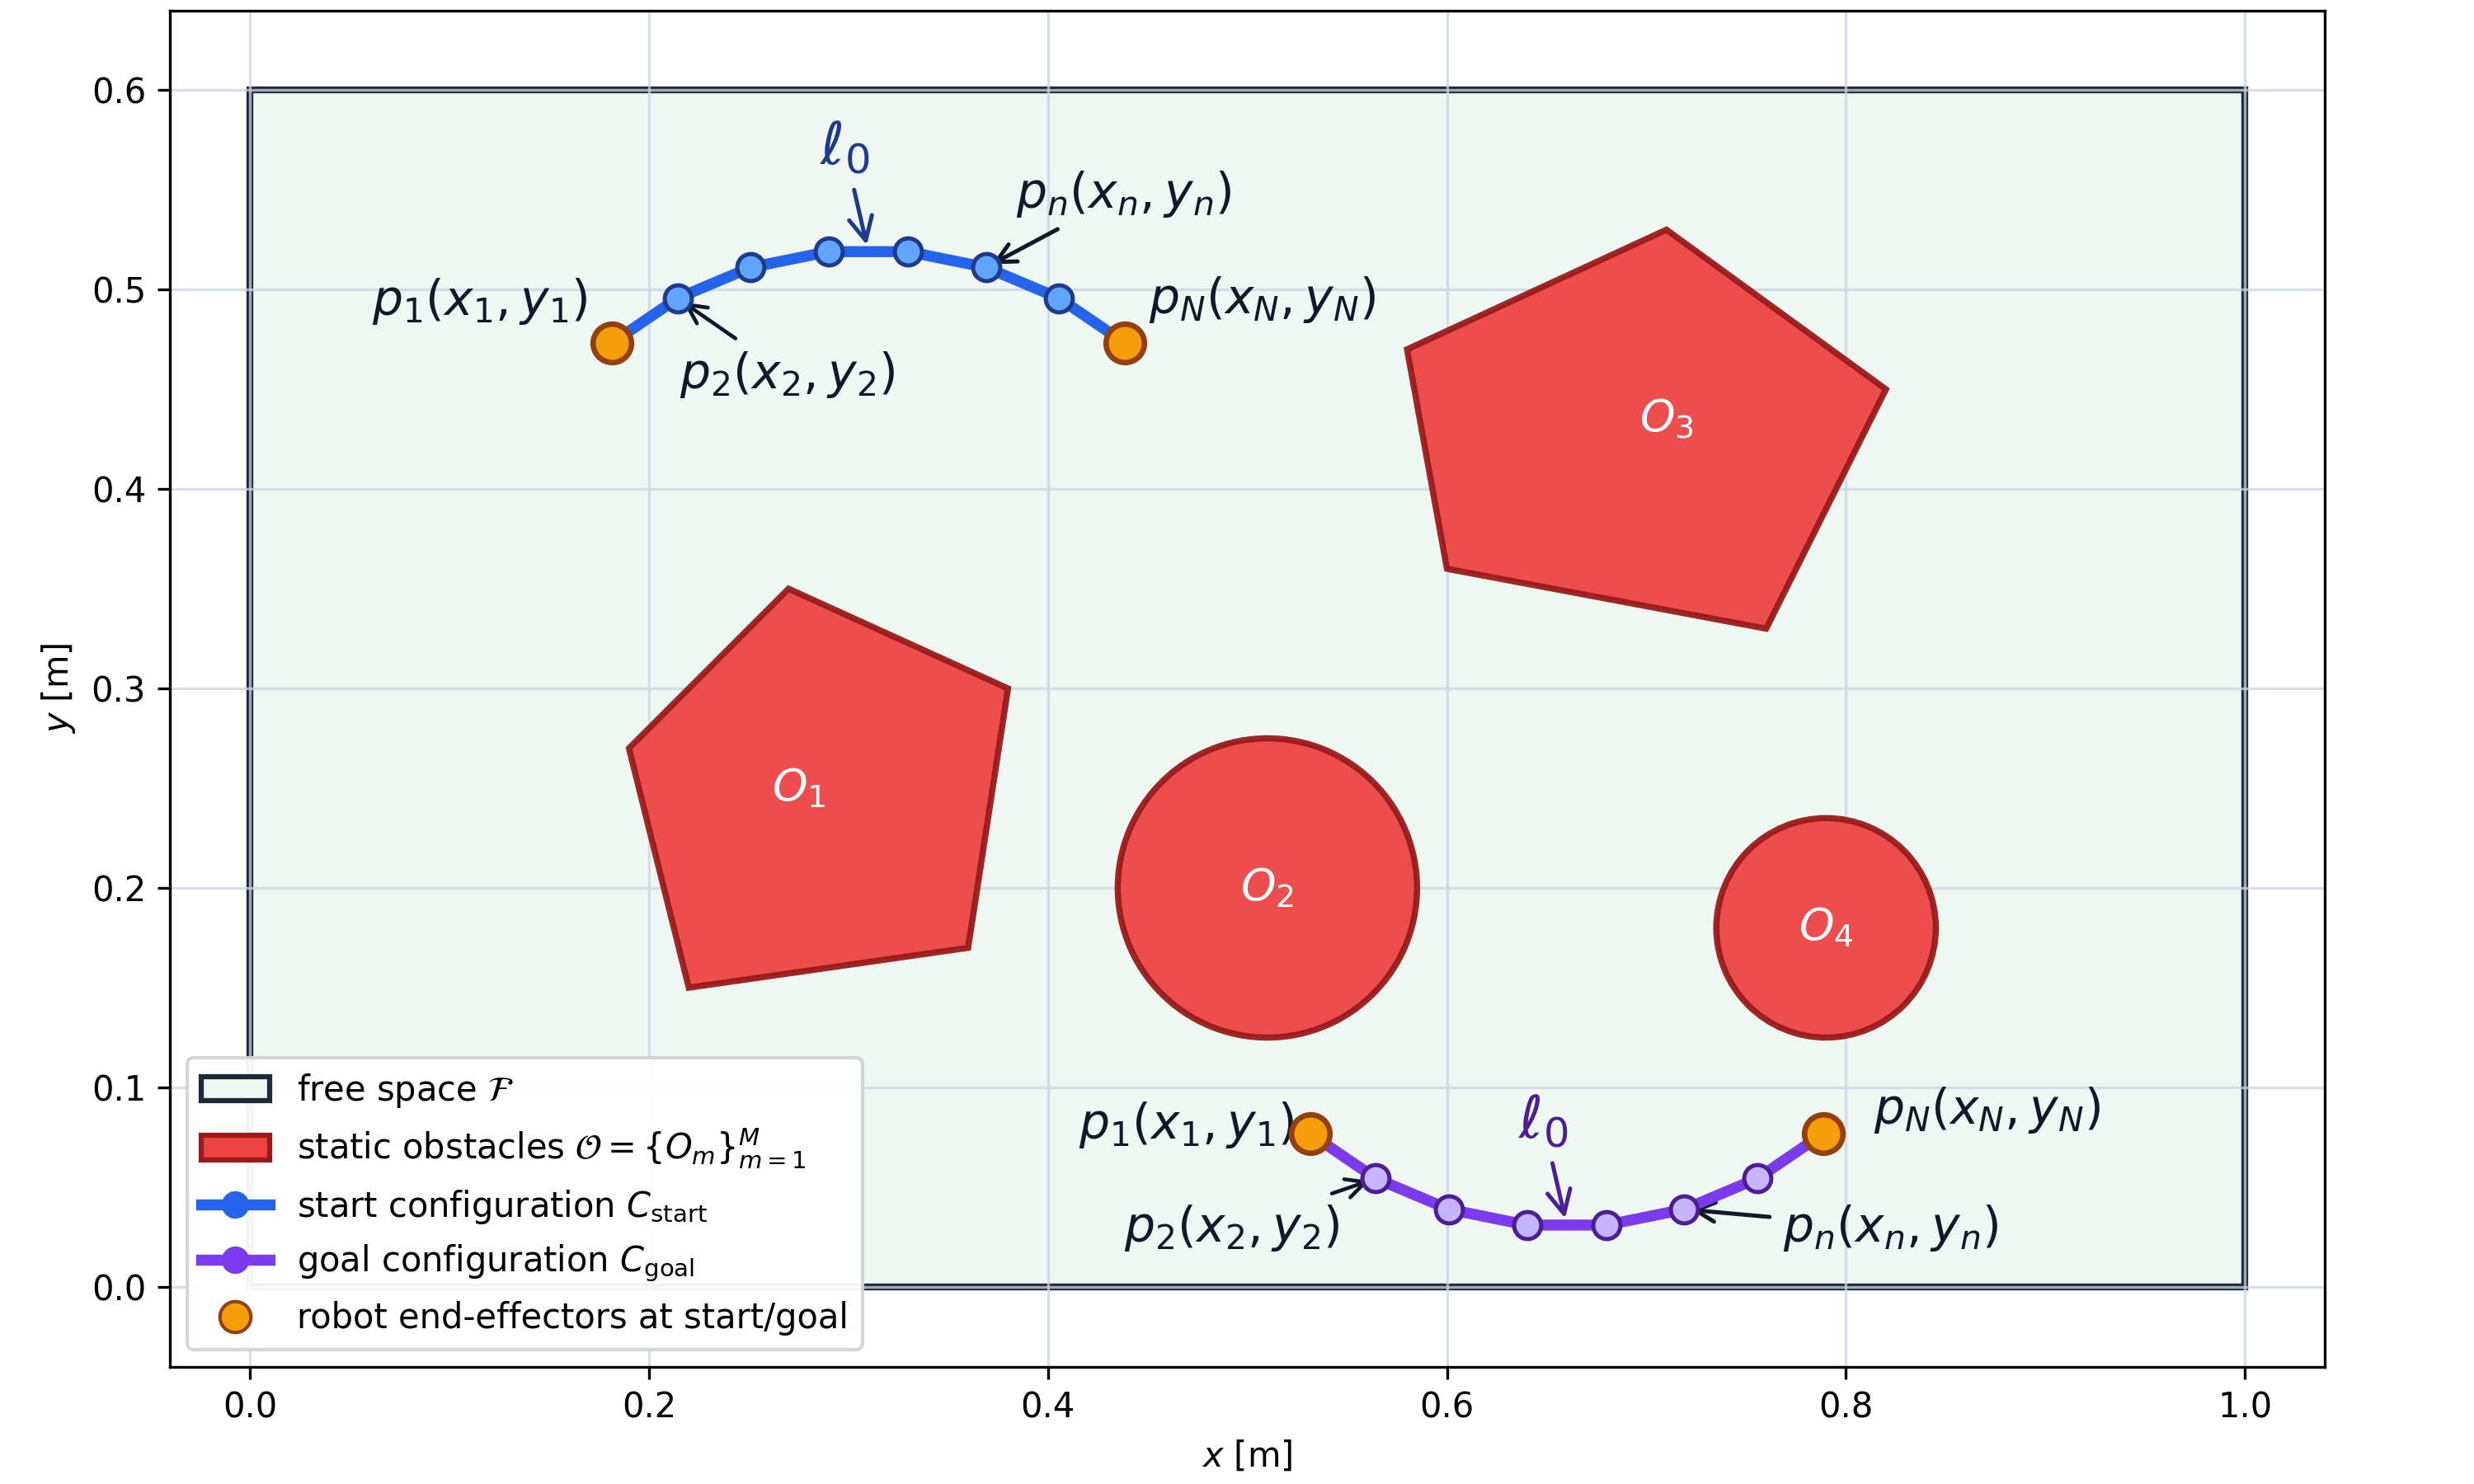
\includegraphics[width=0.5\textwidth]{figures/dlo_workspace_problem_formulation.png}
    \caption{Problem formulation for global cable routing in a planar workspace with static obstacles.}
    \label{fig:dlo_workspace_problem_formulation}
\end{figure}

\subsection{Local Deformation Measures}
\label{subsec:gcr_elastic_deformation_measures}

The planner does not simulate the full dynamic behavior of the cable during
search. Instead, it uses local geometric deformation measures to describe how
the cable shape changes between two configurations. These measures are based on
segment-vector variation and discrete-curvature variation. They are used both to
regularize candidate configurations during relaxation and to evaluate the
deformation cost of accepted planning edges.

For a cable configuration
\begin{equation}
C=(p_1,p_2,\ldots,p_N),
\end{equation}
the vector of the \(k\)-th cable segment is defined as
\begin{equation}
v_k(C)=p_{k+1}-p_k,
\qquad
k=1,\ldots,N-1.
\label{eq:gcr_segment_vector}
\end{equation}
This vector represents both the local length and the local orientation of the
cable segment. Therefore, changes in \(v_k(C)\) describe local stretching,
compression, and rotation of the corresponding cable element.

Local bending is described by the second-order finite difference
\begin{equation}
b_k(C)=p_{k+2}-2p_{k+1}+p_k,
\qquad
k=1,\ldots,N-2.
\label{eq:gcr_discrete_curvature}
\end{equation}
This quantity measures the local change of direction along the cable. Larger
values correspond to sharper local curvature, while smaller values correspond to
smoother local shapes.

Let
\begin{equation}
C^a=(p^a_1,p^a_2,\ldots,p^a_N),
\qquad
C^b=(p^b_1,p^b_2,\ldots,p^b_N)
\end{equation}
be two cable configurations with the same number of nodes. The segment-vector
change between them is
\begin{equation}
\Delta v_k(C^a,C^b)
=
v_k(C^a)-v_k(C^b),
\qquad
k=1,\ldots,N-1,
\label{eq:gcr_segment_vector_change}
\end{equation}
and the curvature change is
\begin{equation}
\Delta b_k(C^a,C^b)
=
b_k(C^a)-b_k(C^b),
\qquad
k=1,\ldots,N-2.
\label{eq:gcr_curvature_change}
\end{equation}

The local deformation energy between the two configurations is then defined as
\begin{equation}
E_{\mathrm{def}}(C^a,C^b)
=
\lambda_s
\sum_{k=1}^{N-1}
\left\|
\Delta v_k(C^a,C^b)
\right\|^2
+
\lambda_b
\sum_{k=1}^{N-2}
\left\|
\Delta b_k(C^a,C^b)
\right\|^2,
\label{eq:gcr_transition_deformation_energy}
\end{equation}
where \(\lambda_s>0\) and \(\lambda_b>0\) weight the preservation of local
segment structure and local curvature, respectively.

A small value of \(E_{\mathrm{def}}(C^a,C^b)\) indicates that the transition
preserves the local segment lengths, segment directions, and curvature of the
cable. A large value indicates an abrupt local deformation, such as excessive
stretching, compression, rotation, or bending. Therefore, \(E_{\mathrm{def}}\)
is used as the deformation penalty in edge-cost computation and path-quality
evaluation.
Figure~\ref{fig:local-deformation-measures} separates these local terms into
the segment-vector definition, the corresponding vector change between two
neighboring configurations, and the local bending change.

\begin{figure}[ht]
    \centering
    \subfloat[Corresponding segment vectors in \(C^a\) and \(C^b\).]{
    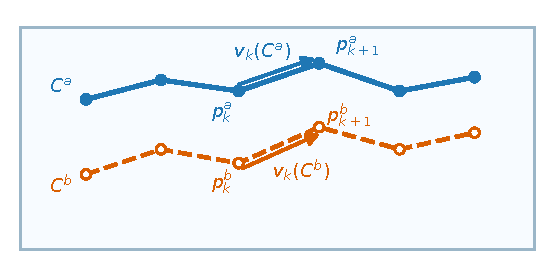
\includegraphics[width=0.9\linewidth]{figures/A_segment_vector_colored.pdf}\label{fig:local-deformation-segment-vector}}
    \hfill \\
    \subfloat[Segment-vector change \(\Delta v_k\).]{
    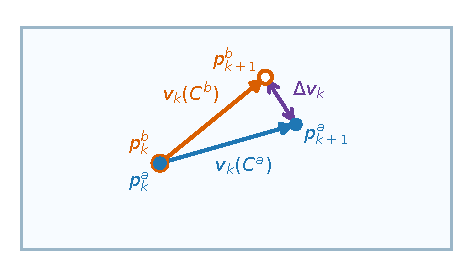
\includegraphics[width=0.5\linewidth]{figures/B_segment_vector_change_colored.pdf}\label{fig:local-deformation-segment-change}}
     ~ \subfloat[Local bending change \(\Delta b_k\).]{
    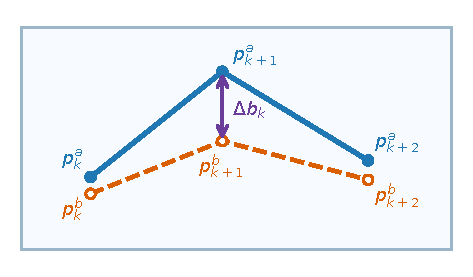
\includegraphics[width=0.5\linewidth]{figures/C_bending_change_colored.pdf}\label{fig:local-deformation-bending-change}}
    \caption{Local deformation measures between two neighboring cable configurations. Blue solid curves denote \(C^a\), orange dashed curves denote \(C^b\), and the difference arrows indicate the local vector and bending terms that enter the deformation penalty.}
    \label{fig:local-deformation-measures}
\end{figure}

The same measure is also used during elastic relaxation. In that case, one of
the two configurations is the candidate configuration being optimized, and the
other is a reference configuration \(C^{\mathrm{ref}}\).
% $E_{\mathrm{def}}(C,C^{\mathrm{ref}})$.
% \begin{equation}
% E_{\mathrm{def}}(C,C^{\mathrm{ref}})
% =
% \lambda_s
% \sum_{k=1}^{N-1}
% \left\|
% v_k(C)-v_k(C^{\mathrm{ref}})
% \right\|^2
% +
% \lambda_b
% \sum_{k=1}^{N-2}
% \left\|
% b_k(C)-b_k(C^{\mathrm{ref}})
% \right\|^2.
% \label{eq:gcr_reference_deformation_energy}
% \end{equation}
This reference-based form reflects the local nature of the planning problem.
Minimizing an absolute stretching--bending energy alone could return a smooth,
low-energy shape that lies far from the previous feasible configuration and
therefore requires an unnecessarily large deformation along a single planning
edge. Since each edge in GCR represents a local manipulation step, deformation
is instead evaluated relative to a nearby feasible configuration: the planner
preserves local cable structure while still allowing the shape to change when
obstacle avoidance or tree expansion requires it.



% ------------------------------------------------------------
\subsection{Admissible and Collision-Free Configurations}
\label{subsec:configuration_space}

A cable configuration is considered statically admissible with respect to a reference configuration when it satisfies three conditions. First, all cable nodes must lie inside the workspace. Second, the deformation of each cable segment must remain bounded with respect to that reference. Third, no cable segment may intersect the obstacle region. As in Section~\ref{subsec:gcr_elastic_deformation_measures}, the reference is a nearby feasible configuration selected during tree expansion, so the admissibility test is local to the proposed planning edge.

% Let
% \[
% C=(p_1,p_2,\ldots,p_N)
% \]
% be a cable configuration, and let
% \[
% C^{\mathrm{ref}}
% =
% (p_1^{\mathrm{ref}},p_2^{\mathrm{ref}},\ldots,p_N^{\mathrm{ref}})
% \]
% be the reference configuration used to evaluate local deformation. The segment vector of the \(k\)-th cable segment is
% \[
% v_k(C)=p_{k+1}-p_k,
% \qquad k=1,\ldots,N-1.
% \]
% The change of this segment relative to the reference configuration is measured by
% \[
% \Delta v_k(C)
% =
% v_k(C)-v_k(C^{\mathrm{ref}})
% \]
Let \(C^{\mathrm{ref}}\) denote the feasible reference configuration used to
evaluate local deformation. To prevent excessive stretching, compression, or
local rotation, the segment-vector deviation \(\Delta v_k(C,C^{\mathrm{ref}})\)
defined in \eqref{eq:gcr_segment_vector_change} is bounded as
\begin{equation}
\|\Delta v_k(C, C^{\mathrm{ref}})\|
\leq
\delta_{\ell},
\qquad
k=1,\ldots,N-1,
\label{eq:segment_vector_displacement_bound}
\end{equation}
where \(\delta_{\ell}>0\) is the maximum allowed local segment-vector deviation. Since this bound is evaluated relative to \(C^{\mathrm{ref}}\), the admissible set is reference-dependent. We write
\begin{equation}
\begin{aligned}
\mathcal{C}_{\mathrm{free}}(C^{\mathrm{ref}})
= &
\left\{
C\in\mathbf{X}
\ \middle|\
\right.
p_n\in\mathcal{W},
& n=1,\ldots,N,
\\
&
\|\Delta  v_k(C, C^{\mathrm{ref}})\|
\leq
\delta_{\ell},
& k=1,\ldots,N-1,
\\
&
s_k(C)\cap\mathcal{O}=\emptyset,
& \left. k=1,\ldots,N-1
\right\}
\end{aligned}
\label{eq:collision_free_configuration_space}
\end{equation}
and use \(\mathcal{C}_{\mathrm{free}}\) as shorthand when the reference
configuration is clear from context.
Figure~\ref{fig:admissible-collision-free} illustrates these tests by comparing
one accepted candidate with two rejected cases: one violates the local
segment-vector bound, and one intersects an obstacle.

\begin{figure}[ht]
    \centering
    \subfloat[Accepted admissible configuration.]{
    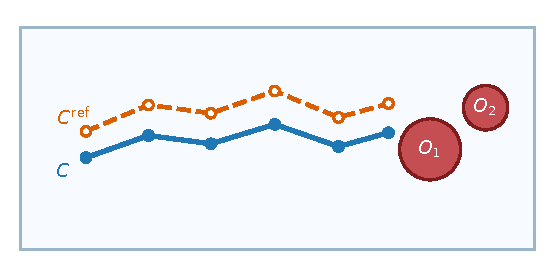
\includegraphics[width=0.9\linewidth]{figures/A_accepted_colored.pdf}\label{fig:admissible-accepted}}
    \hfill \\
    \subfloat[Local-bound violation.]{
    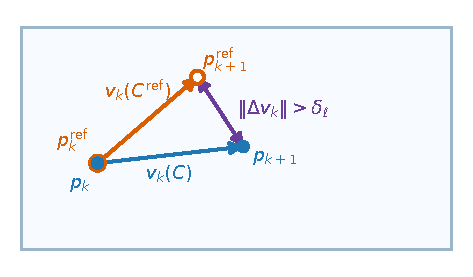
\includegraphics[width=0.5\linewidth]{figures/B_deformation_bound_fails_colored.pdf}\label{fig:admissible-deformation-bound-fails}}
    \subfloat[Rejected by cable-obstacle intersection.]{
    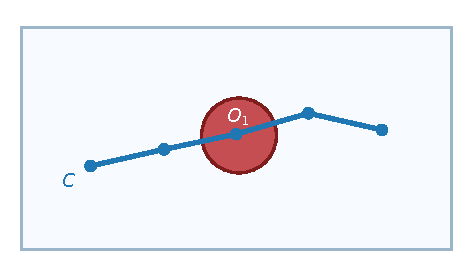
\includegraphics[width=0.5\linewidth]{figures/C_collision_fails_colored.pdf}\label{fig:admissible-collision-fails}}
    \caption{Schematic examples of static configuration validity. Blue curves denote the candidate configuration, orange dashed curves denote the reference configuration where applicable, and red regions denote obstacles. The rejected cases violate either the local bound \(\|\Delta v_k\|\leq\delta_\ell\) or the collision-free segment condition \(s_k(C)\cap\mathcal{O}=\emptyset\).}
    \label{fig:admissible-collision-free}
\end{figure}

This definition checks the complete polygonal representation of the cable, not only its discrete nodes. In particular, obstacle avoidance is verified for every segment
\[
s_k(C)=[p_k,p_{k+1}],
\]
which prevents collisions along the cable configuration between neighboring nodes.

To measure the safety margin between the cable and the obstacles, we use a signed obstacle distance. For a point \(x\in\mathbb{R}^{2}\), this distance is defined as
\begin{equation}
d_{\mathcal{O}}(x)
=
\begin{cases}
\operatorname{dist}(x,\partial\mathcal{O}), & x\notin\mathcal{O},\\
0, & x\in\partial\mathcal{O},\\
-\operatorname{dist}(x,\partial\mathcal{O}), & x\in\mathcal{O}.
\end{cases}
\label{eq:signed_obstacle_distance}
\end{equation}
Thus, a positive value indicates that the point is outside the obstacle region, a zero value indicates contact with the obstacle boundary, and a negative value indicates penetration into an obstacle.

The clearance of a complete cable configuration is evaluated by sampling points along all cable segments and taking the smallest signed distance among them. For the \(q\)-th sample on segment \(s_k(C)\), let
\[
x_{kq}(C)
=
(1-\rho_q)p_k+\rho_q p_{k+1},
\qquad
\rho_q=\frac{q}{Q},
\qquad
q=0,\ldots,Q.
\]
The configuration clearance is then
\begin{equation}
\operatorname{clear}(C)
=
\min_{\substack{k=1,\ldots,N-1\\ q=0,\ldots,Q}}
d_{\mathcal{O}}\!\left(x_{kq}(C)\right).
\label{eq:configuration_clearance}
\end{equation}

In particular, a negative clearance indicates that at least one sampled point lies inside an obstacle and the configuration is in collision.

% ------------------------------------------------------------
\subsection{Configuration Distance and Path Cost}
\label{subsec:distance_path_cost}

The distance between two cable configurations is measured by the maximum
point-wise displacement of corresponding cable nodes:
\begin{equation}
d(C_i,C_j)
=
\max_{1\leq n\leq N}
\left\|
p_n^{i}-p_n^{j}
\right\|.
\label{eq:configuration_distance_metric}
\end{equation}
This metric limits the largest motion of any discretized cable point during a
local transition. It is therefore suitable for nearest-neighbor search,
connection-radius tests, local edge evaluation, and path-cost computation.

A discrete cable path is represented as a finite sequence of configurations,
\begin{equation}
\mathcal{P}
=
\{C_0,C_1,\ldots,C_K\},
\qquad
C_0=C_{\mathrm{start}},
\qquad
C_K=C_{\mathrm{goal}} .
\label{eq:discrete_cable_path}
\end{equation}
Each consecutive pair \((C_i,C_{i+1})\) defines one local deformation of the
cable. The geometric length of the path is computed as
\begin{equation}
J_{\mathrm{geom}}(\mathcal{P})
=
\sum_{i=0}^{K-1}
d(C_i,C_{i+1}).
\label{eq:path_geometric_cost}
\end{equation}

In addition to geometric displacement, the planner penalizes deformation between
consecutive cable configurations. The deformation cost of the path is defined as
\begin{equation}
J_{\mathrm{def}}(\mathcal{P})
=
\sum_{i=0}^{K-1}
E_{\mathrm{def}}(C_{i+1},C_i),
\label{eq:path_deformation_cost}
\end{equation}
where \(E_{\mathrm{def}}\) is the local deformation energy defined in
\eqref{eq:gcr_transition_deformation_energy}.

The complete path objective combines the geometric motion cost and the
deformation cost:
\begin{equation}
J(\mathcal{P})
=
J_{\mathrm{geom}}(\mathcal{P})
+
\alpha_{\mathrm{def}}
J_{\mathrm{def}}(\mathcal{P}),
\label{eq:complete_path_cost_objective}
\end{equation}
% or equivalently,
% \begin{equation}
% J(\mathcal{P})
% =
% \sum_{i=0}^{K-1}
% \left[
% d(C_i,C_{i+1})
% +
% \alpha_{\mathrm{def}}
% E_{\mathrm{def}}(C_{i+1},C_i)
% \right],
% \label{eq:path_cost_objective}
% \end{equation}
where \(\alpha_{\mathrm{def}}\geq 0\) is a weighting coefficient that controls
the relative importance of deformation minimization.

The first term favors short transitions in configuration space, while the second
term favors smooth and mechanically plausible cable deformation.
Figure~\ref{fig:configuration-distance-cost} summarizes the max-norm edge
metric and the accumulation of accepted local transition costs along a discrete
cable path.

\begin{figure}[ht]
    \centering
    \subfloat[Edge-distance metric.]{
    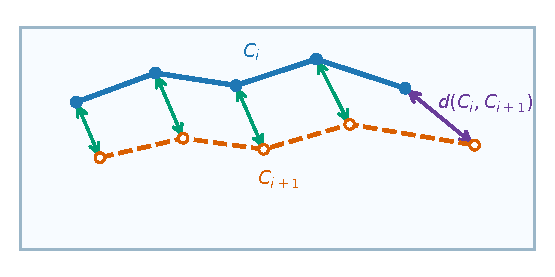
\includegraphics[width=0.9\linewidth]{figures/A_edge_distance_colored.pdf}\label{fig:configuration-edge-distance}}
    \hfill \\
    \subfloat[Accumulated path cost.]{
    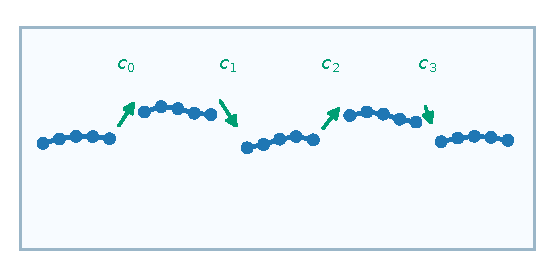
\includegraphics[width=0.9\linewidth]{figures/B_accumulated_path_cost_colored.pdf}\label{fig:configuration-accumulated-path-cost}}
    \caption{Configuration distance and accumulated path cost. The edge-distance panel depicts the max-norm metric \(d(C_i,C_{i+1})=\max_n\|p_n^i-p_n^{i+1}\|\), for which the edge length is induced by the largest displacement among corresponding cable nodes. The path-cost panel shows the accumulation \(J(\mathcal{P})=\sum_i c_i\), where \(c_i=d(C_i,C_{i+1})+\alpha_{\mathrm{def}}E_{\mathrm{def}}(C_{i+1},C_i)\).}
    \label{fig:configuration-distance-cost}
\end{figure}
% ------------------------------------------------------------
\subsection{Transition Feasibility}
\label{subsec:continuous_motion}

Static feasibility of individual cable configurations is not sufficient for
cable manipulation. Even if two configurations are separately collision-free,
the motion between them may pass through an obstacle. Therefore, every edge
between two neighboring configurations must be checked for transition
feasibility.

Let
\[
C^a=(p_1^a,p_2^a,\ldots,p_N^a),
\qquad
C^b=(p_1^b,p_2^b,\ldots,p_N^b)
\]
be two cable configurations. During the transition from \(C^a\) to \(C^b\),
the cable occupies a swept region in the workspace. The swept region is
evaluated with respect to the ordered point correspondence
\(p_n^a\leftrightarrow p_n^b\). For the \(k\)-th segment, a conservative
planar swept envelope is the convex hull of the segment before and after the
local deformation:
\begin{equation}
\mathcal{E}_{ab}^{(k)}
=
\operatorname{conv}
\left\{
p_k^{a},p_{k+1}^{a},p_{k+1}^{b},p_k^{b}
\right\},
\qquad
k=1,\ldots,N-1 .
\label{eq:segment_swept_envelope}
\end{equation}
The swept envelope of the complete cable transition is then
\begin{equation}
\mathcal{E}_{ab}
=
\bigcup_{k=1}^{N-1}
\mathcal{E}_{ab}^{(k)} .
\label{eq:swept_polygon_formulation}
\end{equation}
This segment-wise definition avoids relying on a single full-chain polygon when
the two cable configurations are folded or when their outer envelope would be
self-intersecting. It also makes explicit that the transition depends on the
chosen ordering of corresponding nodes.

The transition is considered deformation-feasible if this swept envelope does
not intersect the obstacle region:
\begin{equation}
\mathcal{E}_{ab}\cap\mathcal{O}
=
\emptyset .
\label{eq:swept_envelope_free_condition}
\end{equation}

Accordingly, we define the binary swept-clear indicator
\begin{equation}
\chi_{\mathrm{sw}}(C^a,C^b)
=
\begin{cases}
1, & \mathcal{E}_{ab}\cap\mathcal{O}=\emptyset,\\
0, & \mathrm{otherwise}.
\end{cases}
\label{eq:swept_clear_indicator_definition}
\end{equation}

Figure~\ref{fig:transition-feasibility} contrasts a clear swept envelope with a
blocked one: obstacle avoidance is checked for the continuous local
deformation, not only at the two endpoint configurations.

\begin{figure}[ht]
    \centering
    \subfloat[Clear swept envelope.]{
    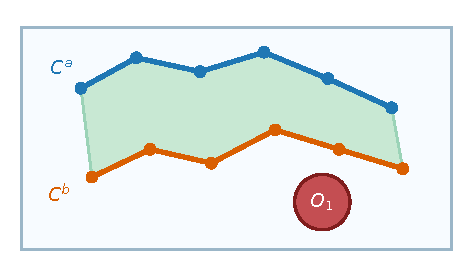
\includegraphics[width=0.9\linewidth]{figures/A_swept_region_clear_colored.pdf}\label{fig:transition-swept-clear}}
    \hfill \\
    \subfloat[Blocked swept envelope.]{
    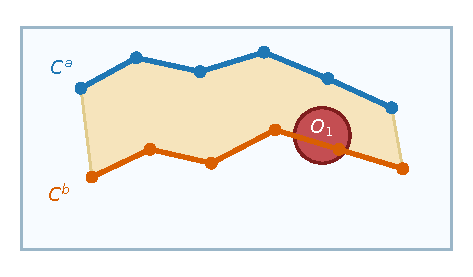
\includegraphics[width=0.9\linewidth]{figures/B_swept_region_blocked_colored.pdf}\label{fig:transition-swept-blocked}}
    \caption{Transition feasibility between two ordered configurations. Blue and orange curves denote the two neighboring cable shapes, the shaded band is the swept envelope, and red regions denote obstacles. The complete edge is accepted only when the swept region is obstacle-free and the remaining conditions in \(\Gamma(\cdot,\cdot)\) are also satisfied.}
    \label{fig:transition-feasibility}
\end{figure}


\subsection{Ordered Transition Feasibility and Endpoint Correspondence}
\label{subsec:ordered_transition_feasibility}

The swept envelope in \eqref{eq:swept_polygon_formulation} is built from the
point-to-point correspondence \(p_n^a\leftrightarrow p_n^b\), so transition
feasibility depends on the assumed node ordering and not only on the geometric
shapes of the two configurations. The ordering also determines which cable
endpoint is associated with which robot end-effector. This subsection makes the
role of the ordering explicit.

For a cable configuration
\begin{equation}
C=(p_1,p_2,\ldots,p_N),
\end{equation}
we define the reversal operator
\begin{equation}
R(C)=(p_N,p_{N-1},\ldots,p_1).
\label{eq:reversal_operator}
\end{equation}
The configurations $C$ and $R(C)$ describe the same occupied polygonal chain.
Therefore, for static collision checking, they are geometrically equivalent.
However, they do not necessarily define the same transition when connected to
another ordered configuration.

Let
\begin{equation}
C=(p_1,p_2,\ldots,p_N),
\qquad
D=(q_1,q_2,\ldots,q_N)
\end{equation}
be two ordered cable configurations. The swept-clear indicator is ordered:
\(\chi_{\mathrm{sw}}(C,D)\) assumes that point $p_n$ moves toward point
$q_n$ for all $n=1,\ldots,N$. Thus, the transition is defined by the ordered
correspondence
\begin{equation}
p_n \longleftrightarrow q_n,
\qquad n=1,\ldots,N.
\end{equation}
If one of the two configurations is reversed, this correspondence changes. For
example, the transition from $R(C)$ to $D$ connects $p_{N-n+1}$ to $q_n$,
which may generate a different swept region from the one generated by the
transition from $C$ to $D$.

This motivates the following observation.

\textbf{Lemma: Simultaneous Reversal Invariance.}
Let $C$ and $D$ be two ordered cable configurations. Then
\begin{equation}
\chi_{\mathrm{sw}}(C,D)
=
\chi_{\mathrm{sw}}(R(C),R(D)).
\end{equation}

\textit{Proof.}
The transition from $C$ to $D$ connects each point $p_n$ to the corresponding
point $q_n$. If both configurations are reversed, the same geometric
correspondence is preserved under the index substitution
$n \mapsto N-n+1$. Therefore, the swept region generated by the ordered pair
$(C,D)$ is identical to the swept region generated by the ordered pair
$(R(C),R(D))$. Since the obstacle set is unchanged, the collision result is also
unchanged. Hence
\begin{equation}
\chi_{\mathrm{sw}}(C,D)
=
\chi_{\mathrm{sw}}(R(C),R(D)).
\end{equation}

In contrast, the invariance does not extend to the case where only one
configuration is reversed. In general,
\begin{equation}
\chi_{\mathrm{sw}}(C,D)
\neq
\chi_{\mathrm{sw}}(R(C),D),
\end{equation}
and
\begin{equation}
\chi_{\mathrm{sw}}(C,D)
\neq
\chi_{\mathrm{sw}}(C,R(D)).
\end{equation}
In such cases, the swept envelope may become larger, self-intersecting, or
cover a different part of the workspace, so a transition that is collision-free
under one ordering may be invalid under another.
Figure~\ref{fig:order-transition-endpoint-correspondence} illustrates this
dependence on endpoint correspondence: the same two geometric cable shapes can
produce different swept regions when one ordering is changed.

\begin{figure}[ht]
    \centering
    \subfloat[Swapped endpoint correspondence.]{
    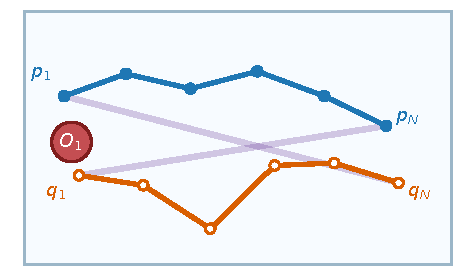
\includegraphics[width=0.9\linewidth]{figures/A_swapped_endpoints_colored.pdf}\label{fig:order-transition-swapped-endpoints}}
    \hfill \\
    \subfloat[Preserved endpoint correspondence.]{
    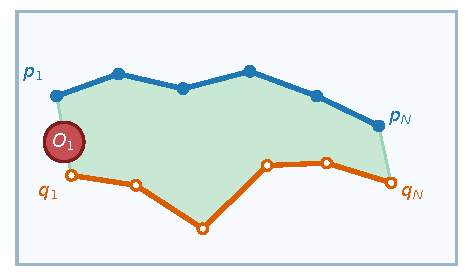
\includegraphics[width=0.9\linewidth]{figures/B_preserved_endpoints_colored.pdf}\label{fig:order-transition-preserved-endpoints}}
    \caption{Endpoint correspondence for ordered cable transitions. The same two cable shapes can produce different swept regions under different endpoint correspondences. In this schematic example, the swapped correspondence produces an X-shaped sweep away from the obstacle, whereas the preserved correspondence intersects the obstacle; therefore, \(\chi_{\mathrm{sw}}\) and \(\Gamma\) must be evaluated using the ordered representatives actually used by the planner.}
    \label{fig:order-transition-endpoint-correspondence}
\end{figure}

For this reason, transition feasibility must be evaluated for the actual ordered
representatives used by the planner. We introduce the endpoint-order variable
\begin{equation}
\sigma \in \{+1,-1\},
\end{equation}
where
\begin{equation}
C^{\sigma}=
\begin{cases}
C, & \sigma=+1,\\
R(C), & \sigma=-1.
\end{cases}
\end{equation}
An ordered transition from $C^{\sigma_C}$ to $D^{\sigma_D}$ is admissible only
if the swept-envelope condition is satisfied for this particular choice of
ordering:
\begin{equation}
\chi_{\mathrm{sw}}
\left(
C^{\sigma_C},D^{\sigma_D}
\right)=1.
\end{equation}

In addition to collision-free deformation, the ordered transition should preserve
endpoint consistency. We assume that all ordered configurations considered for
execution satisfy \(p_1\neq p_N\), so that the endpoint axis is well defined.
The ordered endpoint axis of a cable configuration is then defined as
\begin{equation}
u(C)=
\frac{p_N-p_1}{\|p_N-p_1\|}.
\end{equation}
For two ordered configurations $C$ and $D$, the change in endpoint direction is
\begin{equation}
\theta(C,D)
=
\cos^{-1}
\left(
u(C)^{\top}u(D)
\right).
\end{equation}
The ordered transition is considered endpoint-consistent if
\begin{equation}
\theta(C,D)\leq \theta_{\max},
\end{equation}
where $\theta_{\max}$ is the maximum admissible change in the ordered cable
axis.

For compact notation, we define the ordered edge-feasibility predicate by
\begin{equation}
\Gamma(C,D)=1
\quad\Longleftrightarrow\quad
\begin{cases}
\chi_{\mathrm{sw}}(C,D)=1,\\
\theta(C,D)\leq \theta_{\max},\\
\Psi(C,D)=1.
\end{cases}
\label{eq:ordered_edge_feasibility_predicate}
\end{equation}
Here, $\Psi(C,D)$ denotes robot-dependent endpoint feasibility, including
admissible endpoint displacement, endpoint obstacle clearance, and end-effector
motion limits. If robotic execution constraints are not considered during
planning, $\Psi(C,D)$ can be set identically equal to one.

Thus, the ordering used by each accepted tree edge must be fixed
during planning, and the ordered transition predicate $\Gamma(\cdot,\cdot)$
must be evaluated before inserting a new edge into the search tree.



% ============================================================
\section{Global Cable Routing Algorithm}
\label{sec:gcr_algorithm}

The implemented GCR planner is a bidirectional sampling-based planner in the discretized cable configuration space. It grows one tree from \(C_{\mathrm{start}}\) and one tree from \(C_{\mathrm{goal}}\). Each accepted vertex is a statically valid cable configuration, and each accepted edge satisfies the ordered transition predicate \(\Gamma(\cdot,\cdot)\).

% ------------------------------------------------------------
\subsection{Search Trees and Bidirectional Expansion}
\label{subsec:gcr_search_trees}

Let
\begin{equation}
T_s=(V_s,E_s),
\qquad
T_g=(V_g,E_g)
\label{eq:gcr_two_trees}
\end{equation}
denote the start and goal trees. They are initialized as
\begin{equation}
V_s=\{C_{\mathrm{start}}\},
\qquad
V_g=\{C_{\mathrm{goal}}\}.
\label{eq:gcr_tree_initialization}
\end{equation}
The algorithm alternates between the two trees. At odd iterations, \(T_s\) is expanded toward \(C_{\mathrm{goal}}\). At even iterations, \(T_g\) is expanded toward \(C_{\mathrm{start}}\).

For a new accepted configuration \(C^{\mathrm{new}}\) with parent \(C^{\mathrm{par}}\), the stored cost-to-come is
\begin{equation}
g(C^{\mathrm{new}})
=
g(C^{\mathrm{par}})
+
d(C^{\mathrm{par}},C^{\mathrm{new}})
+
\alpha_{\mathrm{def}}
E_{\mathrm{def}}(C^{\mathrm{new}},C^{\mathrm{par}}),
\label{eq:tree_cost_to_come}
\end{equation}
where \(\alpha_{\mathrm{def}}\geq0\) weights the deformation term. This cost is used as an internal edge-quality measure and is consistent with the path objective \(J(\mathcal{P})\) in \eqref{eq:complete_path_cost_objective}.
The corresponding bidirectional structure is shown in
Figure~\ref{fig:bidirectional-search-trees}, where the start and goal trees grow
through the obstacle field and are connected only by a validated bridge.

\begin{figure}[ht]
    \centering
    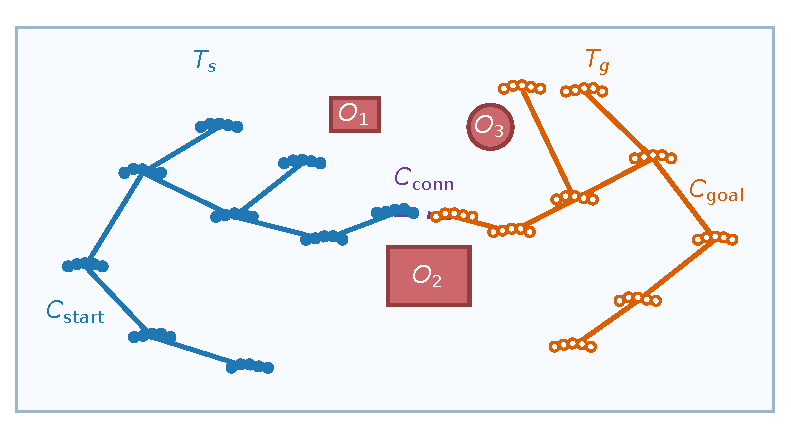
\includegraphics[width=0.95\linewidth]{figures/bidirectional_search_trees_colored.pdf}
    \caption{Bidirectional search-tree structure used by GCR. The blue start tree \(T_s\) is rooted at \(C_{\mathrm{start}}\), and the orange goal tree \(T_g\) is rooted at \(C_{\mathrm{goal}}\). Red regions are obstacles, and the dashed purple bridge denotes the candidate inter-tree connection \(C_{\mathrm{conn}}\). The displayed vertices and edges are collision-free; a bridge is accepted only if the ordered edge-feasibility predicate \(\Gamma\) validates the connection.}
    \label{fig:bidirectional-search-trees}
\end{figure}

% ------------------------------------------------------------
\subsection{Guided Configuration Sampling}
\label{subsec:gcr_guided_sampling}

At each tree-expansion step, the planner generates a raw candidate cable
configuration before applying APF biasing and elastic relaxation. Instead of
sampling only from a uniform distribution over the configuration space, the
proposed method uses a guided mixture sampler. This sampler combines directed
sampling toward the target, local expansion from the active tree, and broad
exploration of the workspace.

The raw configuration is sampled from the mixture distribution
\begin{equation}
C^{\mathrm{raw}}
\sim
p_{\mathrm{goal}}\,\mathcal{Q}_{\mathrm{goal}}
+
p_{\mathrm{tree}}\,\mathcal{Q}_{\mathrm{tree}}
+
p_{\mathrm{broad}}\,\mathcal{Q}_{\mathrm{broad}},
\label{eq:guided_mixture_sampler}
\end{equation}
where \(\mathcal{Q}_{\mathrm{goal}}\), \(\mathcal{Q}_{\mathrm{tree}}\), and
\(\mathcal{Q}_{\mathrm{broad}}\) denote the goal-guided, tree-guided, and broad
exploration sampling distributions, respectively. Their probabilities satisfy
\begin{equation}
p_{\mathrm{goal}}+p_{\mathrm{tree}}+p_{\mathrm{broad}}=1.
\label{eq:guided_sampler_probabilities}
\end{equation}

The goal-guided component \(\mathcal{Q}_{\mathrm{goal}}\) generates candidate
configurations in the neighborhood of the current target configuration
\(C^{\mathrm{target}}\). This component increases the probability of producing
samples that move the search toward the opposite tree. A small perturbation is
added to avoid repeatedly generating identical configurations and to preserve
local exploration around the target shape.

The tree-guided component \(\mathcal{Q}_{\mathrm{tree}}\) expands from an
existing configuration in the active tree. Let \(C^p\in V_{\mathrm{act}}\) be a
selected parent configuration and let \(C^{\ell}\) be a local target
configuration. The base configuration is generated by moving from \(C^p\) toward
\(C^{\ell}\):
\begin{equation}
C^{\mathrm{base}}
=
C^p
+
\alpha
\left(
C^{\ell}-C^p
\right),
\label{eq:tree_biased_base}
\end{equation}
where \(\alpha\in[\alpha_{\min},\alpha_{\max}]\) controls the local expansion
step. It is chosen according to the distance between \(C^p\) and \(C^{\ell}\):
\begin{equation}
\alpha
=
\min
\left\{
\alpha_{\max},
\max
\left\{
\alpha_{\min},
\frac{\gamma \epsilon}{d(C^p,C^{\ell})}
\right\}
\right\},
\label{eq:tree_biased_alpha}
\end{equation}
where \(\epsilon\) is the local connection radius and \(\gamma>0\) is a scaling
coefficient. This rule keeps the sampled configuration within a controlled
neighborhood of the active tree while still directing the expansion toward a
useful local target.

After a base configuration has been selected, local perturbations are applied to
increase sampling diversity. For each cable node, the sampled point is written as
\begin{equation}
p_i^{\mathrm{raw}}
=
p_i^{\mathrm{base}}
+
\xi_i
+
a
\sin
\left(
\frac{\pi(i-1)}{N-1}
\right)
n_i(C^{\mathrm{base}}),
\label{eq:raw_sample_noise}
\end{equation}
where \(\xi_i\) is a small zero-mean Gaussian perturbation, \(a\) is a scalar
lateral perturbation amplitude, and \(n_i(C^{\mathrm{base}})\) is the local
normal direction of the cable at node \(i\). The sinusoidal factor makes the
lateral deformation smooth along the cable and reduces perturbations near the
endpoints.

The broad exploration component \(\mathcal{Q}_{\mathrm{broad}}\) generates a
new cable shape using a random-walk construction. Starting from an initial node,
successive cable nodes are generated as
\begin{equation}
p_{k+1}
=
p_k
+
\ell_0
\begin{bmatrix}
\cos\theta_k\\
\sin\theta_k
\end{bmatrix},
\qquad
k=1,\ldots,N-1,
\label{eq:broad_random_walk_position}
\end{equation}
with the heading angle updated according to
\begin{equation}
\theta_{k+1}
=
\theta_k+\eta_k,
\qquad
\eta_k\sim\mathcal{N}(0,\sigma_\theta^2).
\label{eq:broad_random_walk_angle}
\end{equation}
Here, \(\ell_0\) is the nominal segment length and \(\sigma_\theta\) controls
the smoothness of the generated shape. After generation, the cable is shifted
into the workspace, clipped to the workspace boundaries if necessary, and
projected toward the nominal segment length.

The raw sample drawn from this mixture is generally not yet a useful tree
candidate; it is first refined by the APF biasing step described next.
% ------------------------------------------------------------
\subsection{Configuration-Level Artificial Potential Field Biasing}
\label{subsec:gcr_config_apf_sampling}

After a raw cable configuration is generated by the guided sampler, it is biased
using a configuration-level artificial potential field (APF). The purpose of
this step is to move the sampled cable toward a more promising region of the
configuration space and push it away from obstacles before the constrained relaxation stage.
% The APF attracts the raw sample toward the current target configuration and repels it from obstacle regions.

Let
\[
C^{\mathrm{raw}}
=
(p_1^{\mathrm{raw}},p_2^{\mathrm{raw}},\ldots,p_N^{\mathrm{raw}})
\]
be the raw configuration obtained from the guided mixture sampler in
\eqref{eq:guided_mixture_sampler}. Rather than being inserted directly into the search tree, it is first transformed into an APF-biased configuration
\[
\widehat{C}
=
(\widehat{p}_1,\widehat{p}_2,\ldots,\widehat{p}_N)
\]

Since a cable configuration is represented as
\begin{equation}
C
=
(p_1,p_2,\ldots,p_N)
\in
\mathbb{R}^{2N},
\label{eq:gcr_configuration_for_apf}
\end{equation}
the potential field is defined at the configuration level as a scalar function
\begin{equation}
U:\mathbb{R}^{2N}\rightarrow\mathbb{R}.
\label{eq:gcr_apf_mapping}
\end{equation}
Its gradient is
\begin{equation}
\nabla U(C)
=
\left(
\frac{\partial U}{\partial p_1},
\frac{\partial U}{\partial p_2},
\ldots,
\frac{\partial U}{\partial p_N}
\right),
\label{eq:gcr_apf_gradient_definition}
\end{equation}
and the corresponding artificial force applied to the $n$-th cable point is
\begin{equation}
F_n(C)
=
-
\frac{\partial U}{\partial p_n}
\label{eq:gcr_pointwise_apf_force}
\end{equation}

The total configuration-level potential is defined as
\begin{equation}
U(C)
=
U_{\mathrm{att}}(C,C_{\mathrm{target}})
+
U_{\mathrm{rep}}(C,\mathcal{O})
\label{eq:gcr_total_configuration_potential}
\end{equation}
Here, $C_{\mathrm{target}}$ is the root of the opposite tree. This bidirectional use of the APF is illustrated in Fig.~\ref{fig:apf_bidirectional_sampling}: during start-tree expansion the attractive component pulls the sampled configuration toward $C_{\mathrm{goal}}$ (Fig.~\ref{fig:apf_start_tree_field}), during goal-tree expansion it pulls toward $C_{\mathrm{start}}$ (Fig.~\ref{fig:apf_goal_tree_field}), and in both cases obstacle regions generate high potential values that form repulsive zones around occupied areas.

The attractive term guides the cable toward the target configuration:
\begin{equation}
U_{\mathrm{att}}(C,C_{\mathrm{target}})
=
\frac{k_{\mathrm{att}}}{2}
\sum_{n=1}^{N}
\left\|
p_n-p_n^{\mathrm{target}}
\right\|^2
\label{eq:gcr_attractive_potential}
\end{equation}
where $k_{\mathrm{att}}>0$ is the attractive gain and
\begin{equation}
C_{\mathrm{target}}
=
\left(
p_1^{\mathrm{target}},
p_2^{\mathrm{target}},
\ldots,
p_N^{\mathrm{target}}
\right)
\label{eq:gcr_target_configuration_points}
\end{equation}

The repulsive term pushes the cable away from obstacles. Since collisions may occur along cable segments and not only at cable nodes, each segment is sampled at $Q+1$ points. For segment $s_k(C)$, the $q$-th sampled point is
\begin{equation}
s_{kq}(C)
=
(1-\rho_q)p_k
+
\rho_q p_{k+1},
\
\rho_q
=
\frac{q}{Q},
\
q=0,\ldots,Q
\label{eq:gcr_segment_sample_points}
\end{equation}
The distance from this point to the obstacle region is
\begin{equation}
r_{kq}(C)
=
\operatorname{dist}
\left(
s_{kq}(C),\mathcal{O}
\right)
=
\min_{x\in\mathcal{O}}
\left\|
s_{kq}(C)-x
\right\|
\label{eq:gcr_segment_obstacle_distance}
\end{equation}
The repulsive potential is then written as
\begin{equation}
U_{\mathrm{rep}}(C,\mathcal{O})
=
\sum_{k=1}^{N-1}
\sum_{q=0}^{Q}
\beta
\exp
\left(
-\frac{r_{kq}^{2}(C)}{2\sigma^{2}}
\right),
\label{eq:gcr_repulsive_potential}
\end{equation}
where $\beta>0$ controls the repulsion strength and $\sigma>0$ controls the obstacle influence range.

\begin{figure}[h]
    \centering
    \subfloat[Start-tree APF with attraction toward the goal configuration.
    \label{fig:apf_start_tree_field}]{
    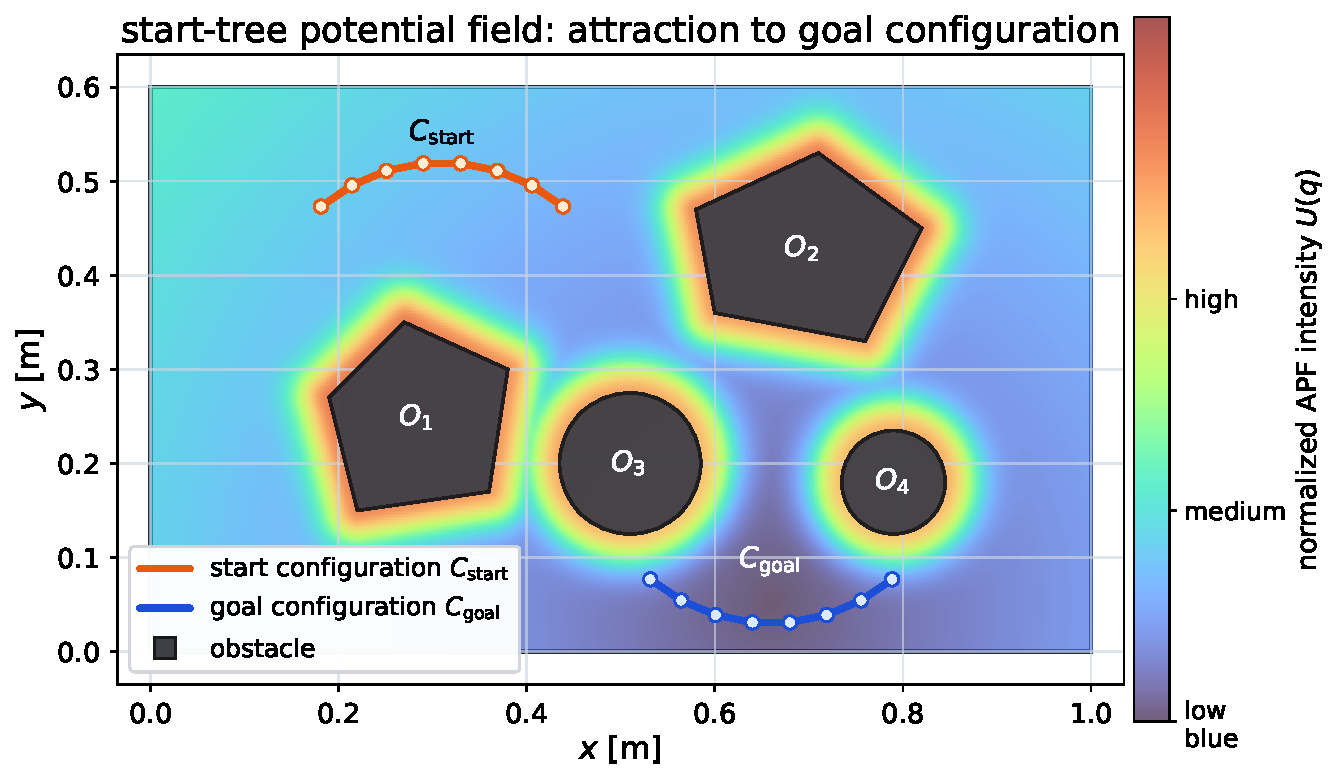
\includegraphics[width=0.75\linewidth]{figures/config_apf_potential_field_start_to_goal.pdf}}
    \\
    \subfloat[Goal-tree APF with attraction toward the start configuration.
    \label{fig:apf_goal_tree_field}]{
    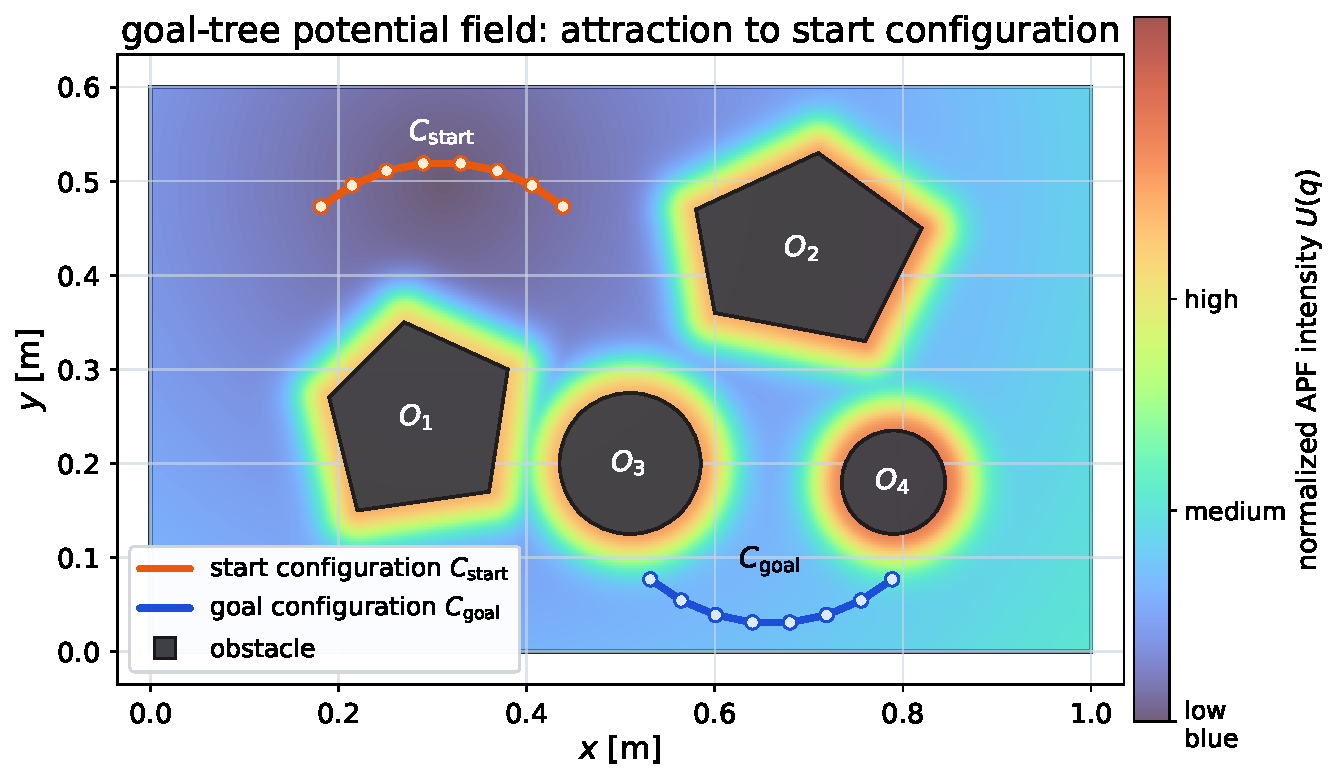
\includegraphics[width=0.75\linewidth]{figures/config_apf_potential_field_goal_to_start.pdf}}
    \caption{Bidirectional configuration-level APF used during tree expansion. The color map represents the normalized potential intensity. Obstacle regions and their neighborhoods correspond to high potential values, while the attractive component biases the expansion toward the opposite tree.}
    \label{fig:apf_bidirectional_sampling}
\end{figure}

Starting from $C^{\mathrm{raw}}$, the APF-biased sample is generated by $H$ gradient descent steps:
\begin{equation}
C^{(h+1)}
=
C^{(h)}
-
\eta
\nabla U(C^{(h)}),
\qquad
h=0,\ldots,H-1,
\label{eq:gcr_apf_gradient_descent}
\end{equation}
with
\begin{equation}
C^{(0)}
=
C^{\mathrm{raw}},
\qquad
\widehat{C}
=
C^{(H)}.
\label{eq:gcr_apf_biased_sample_definition}
\end{equation}
Equivalently, each cable node is updated as
\begin{equation}
p_n^{(h+1)}
=
p_n^{(h)}
+
\eta F_n(C^{(h)}),
\qquad
n=1,\ldots,N.
\label{eq:gcr_pointwise_apf_update}
\end{equation}
where $\eta>0$ is the APF step size.

The local effect of this update is shown in Fig.~\ref{fig:apf_pipeline}. First, a random configuration $C^{\mathrm{raw}}$ is generated in the workspace, as shown in Fig.~\ref{fig:apf_pipeline_raw}. Then, the gradient of the total potential produces pointwise artificial forces acting on the cable nodes, as shown in Fig.~\ref{fig:apf_pipeline_forces}. The raw sample is then transformed into an APF-biased configuration $\widehat{C}$, as shown in Fig.~\ref{fig:apf_pipeline_descent}. The biased configuration is closer to the desired expansion direction and is less likely to pass through high-potential obstacle regions.

The resulting configuration $\widehat{C}$ is not yet guaranteed to satisfy all cable constraints, such as exact segment-length preservation, admissible deformation, or complete collision avoidance; these violations are handled by the relaxation step described next.



\begin{figure}[h]
    \centering
    \subfloat[Sampled raw configuration $C^{\mathrm{raw}}$.
    \label{fig:apf_pipeline_raw}]{
    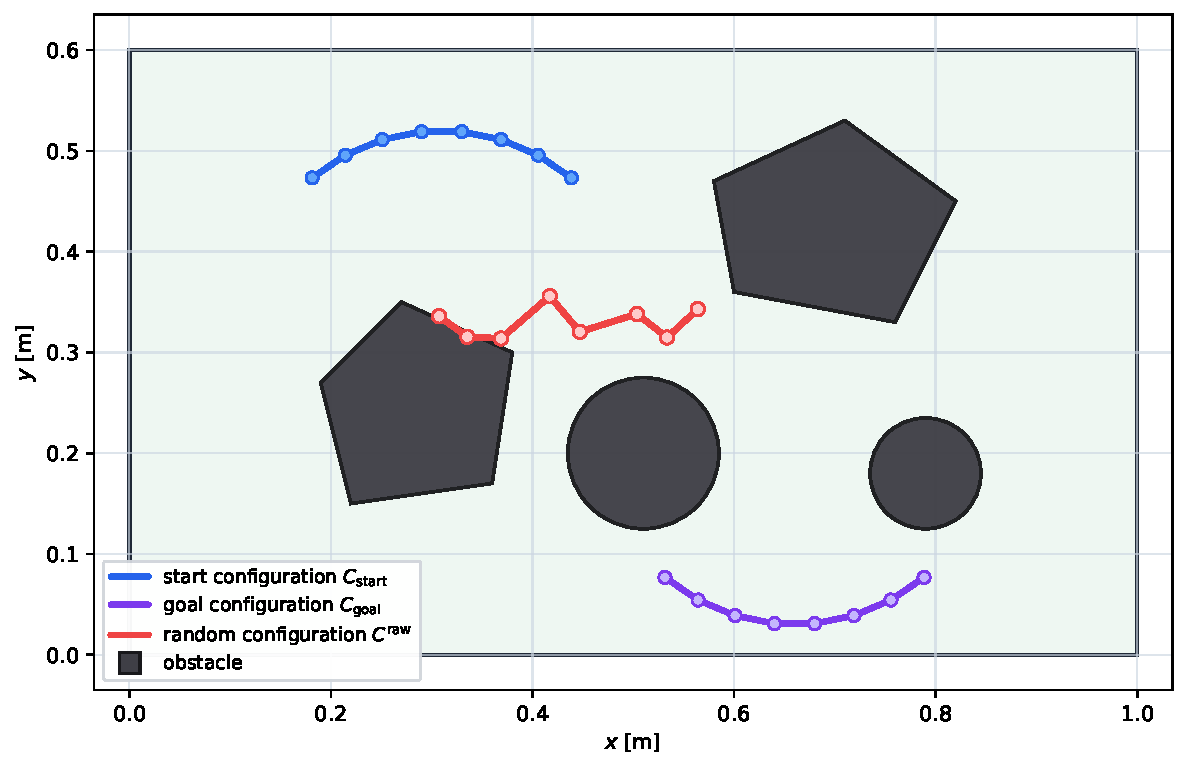
\includegraphics[width=0.8\linewidth]{figures/config_apf_pipeline_step_raw_sample.pdf}}
    \\
    \subfloat[Pointwise artificial forces $F_n(C)$ acting on cable nodes.
    \label{fig:apf_pipeline_forces}]{
    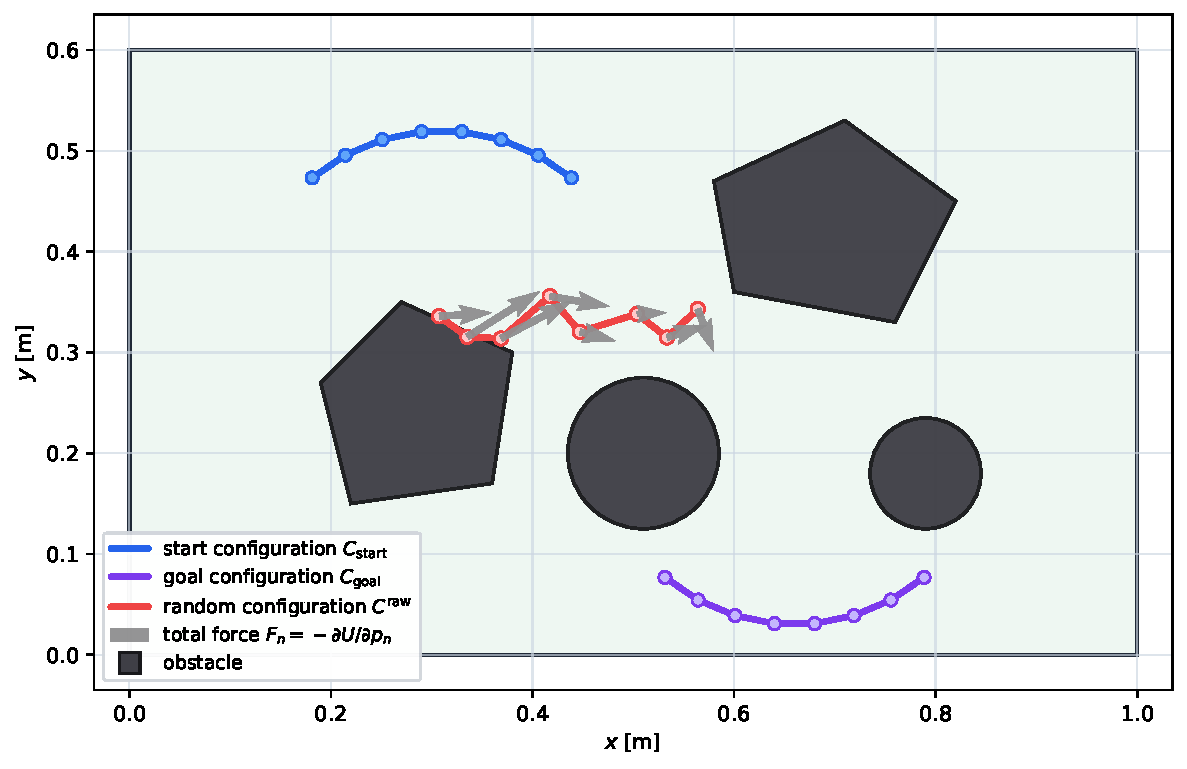
\includegraphics[width=0.8\linewidth]{figures/config_apf_pipeline_step_force_vectors.pdf}}
    \\
    \subfloat[APF-biased configuration $\widehat{C}$ after gradient descent.
    \label{fig:apf_pipeline_descent}]{
    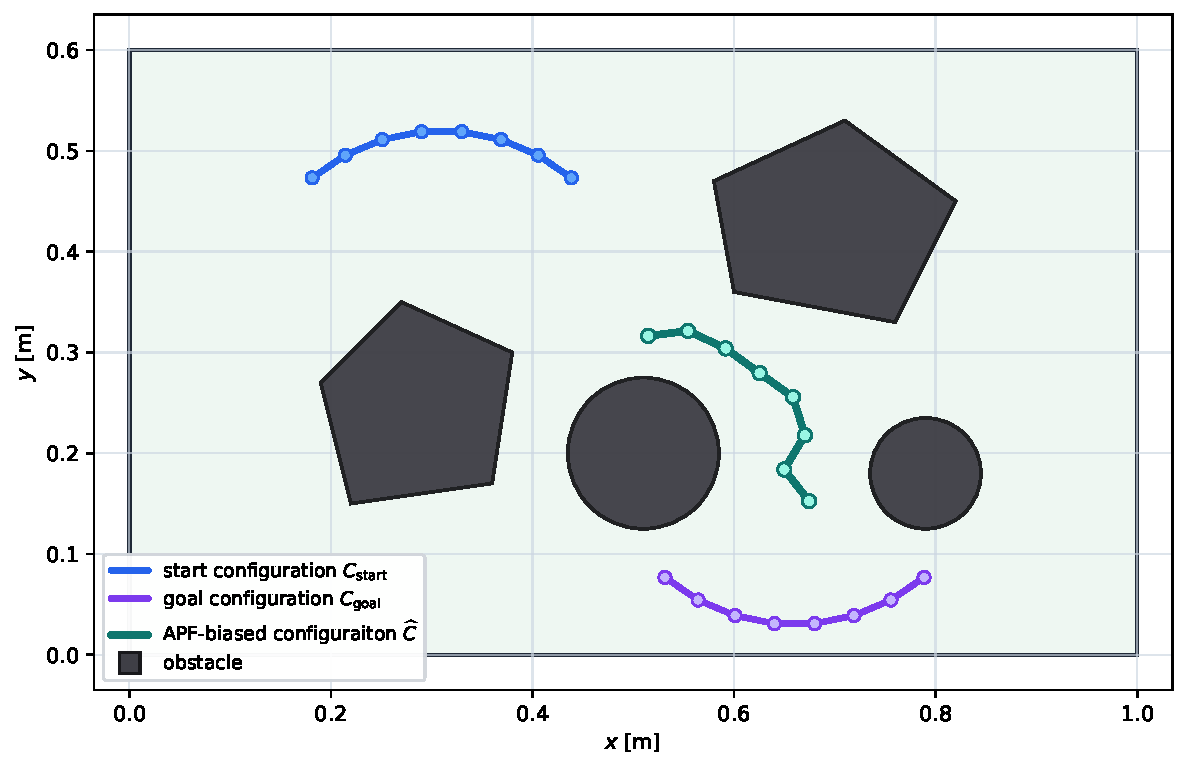
\includegraphics[width=0.8\linewidth]{figures/config_apf_pipeline_step_apf_descent.pdf}}
    \caption{Pipeline of configuration-level APF sampling. A raw random configuration is first generated, then the total APF force is computed for each cable node, and finally the configuration is shifted by gradient descent toward a more promising expansion target.}
    \label{fig:apf_pipeline}
\end{figure}
% ------------------------------------------------------------

% \subsection{Cable Elastic Relaxation}
% \label{subsec:gcr_constrained_relaxation}

% The APF-biased configuration \(\widehat{C}\) is used as a candidate for tree
% expansion. However, this candidate may locally violate deformation limits or
% obstacle-clearance constraints. Therefore, before inserting the candidate into
% the search tree, a projected elastic relaxation step is applied. The purpose of
% this step is to obtain a corrected configuration
% \[
% C^{\mathrm{relax}}
% =
% (p_1^{\mathrm{relax}},p_2^{\mathrm{relax}},\ldots,p_N^{\mathrm{relax}})
% \]
% that remains close to \(\widehat{C}\) while preserving the local shape of a
% reference configuration \(C^{\mathrm{ref}}\).

% Let \(C=(p_1,p_2,\ldots,p_N)\) be the configuration optimized during relaxation.
% The elastic relaxation objective is defined as
% \begin{equation}
% \begin{aligned}
% \Phi(C)
% =
% &
% \frac{w_{\mathrm{tr}}}{2}
% \sum_{n=1}^{N}
% \left\|
% p_n-\widehat{p}_n
% \right\|^2
% +
% \lambda_s
% \sum_{k=1}^{N-1}
% \left\|
% v_k(C)-v_k^{\mathrm{ref}}
% \right\|^2
% \\
% &
% +
% \lambda_b
% \sum_{k=1}^{N-2}
% \left\|
% \Delta^2 p_k-\Delta^2 p_k^{\mathrm{ref}}
% \right\|^2 ,
% \end{aligned}
% \label{eq:relaxation_objective}
% \end{equation}
% where
% \begin{equation}
% v_k(C)=p_{k+1}-p_k,
% \qquad
% v_k^{\mathrm{ref}}=p_{k+1}^{\mathrm{ref}}-p_k^{\mathrm{ref}},
% \label{eq:relaxation_segment_vectors}
% \end{equation}
% and
% \begin{equation}
% \Delta^2 p_k=p_{k+2}-2p_{k+1}+p_k .
% \label{eq:relaxation_second_difference}
% \end{equation}
% The first term keeps the relaxed configuration close to the APF-biased
% configuration, the second term preserves the local segment vectors, and the
% third term preserves the discrete bending profile. The weights
% \(w_{\mathrm{tr}}>0\), \(\lambda_s>0\), and \(\lambda_b>0\) determine the
% relative importance of these objectives.

% The relaxation is initialized as
% \begin{equation}
% C^0=\widehat{C},
% \label{eq:relaxation_initial_condition}
% \end{equation}
% and then updated using projected-gradient iterations. At iteration \(m\), a
% gradient step is first computed:
% \begin{equation}
% C^{m+\frac{1}{2}}
% =
% C^m
% -
% h_{\mathrm{relax}}
% \nabla \Phi(C^m),
% \label{eq:relaxation_gradient_step}
% \end{equation}
% where \(h_{\mathrm{relax}}>0\) is the relaxation step size. The intermediate
% configuration is then projected onto the admissible set:
% \begin{equation}
% C^{m+1}
% =
% \Pi_{\mathrm{end}}
% \Pi_{\mathcal{W}}
% \Pi_{\delta}
% \Pi_{\mathrm{obs}}
% \left(
% C^{m+\frac{1}{2}}
% \right).
% \label{eq:relaxation_projection_step}
% \end{equation}
% Here, \(\Pi_{\mathrm{obs}}\) enforces sampled obstacle-clearance constraints,
% \(\Pi_{\delta}\) limits the deviation of each segment vector from the reference
% configuration, \(\Pi_{\mathcal{W}}\) keeps all cable nodes inside the workspace,
% and \(\Pi_{\mathrm{end}}\) fixes the two endpoints to the APF-biased endpoint
% positions:
% \begin{equation}
% p_1=\widehat{p}_1,
% \qquad
% p_N=\widehat{p}_N .
% \label{eq:relaxation_endpoint_constraint}
% \end{equation}
% The endpoint projection is applied last to guarantee that the endpoint
% displacement generated by the APF step is preserved.

% Obstacle clearance is evaluated at sampled points along each cable segment,
% \begin{equation}
% x_{kq}(C)
% =
% (1-\rho_q)p_k+\rho_q p_{k+1},
% \qquad
% \rho_q=\frac{q}{Q},
% \qquad
% q=0,\ldots,Q .
% \label{eq:relaxation_sampled_points}
% \end{equation}
% The obstacle-clearance projection corrects sampled points that violate the
% safety margin
% \begin{equation}
% d_{\mathcal{O}}\bigl(x_{kq}(C)\bigr) \geq d_{\mathrm{safe}},
% \label{eq:relaxation_clearance_constraint}
% \end{equation}
% where \(d_{\mathcal{O}}(\cdot)\) is the signed obstacle distance and
% \(d_{\mathrm{safe}}>0\) is the required clearance. In the implementation, this
% projection is realized by applying local corrections along the outward obstacle
% normal.

% The segment-deviation projection enforces
% \begin{equation}
% \left\|
% \bigl(p_{k+1}-p_k\bigr)
% -
% \bigl(p_{k+1}^{\mathrm{ref}}-p_k^{\mathrm{ref}}\bigr)
% \right\|
% \leq
% \delta_{\ell},
% \qquad
% k=1,\ldots,N-1 ,
% \label{eq:relaxation_segment_constraint}
% \end{equation}
% where \(\delta_{\ell}\) is the maximum admissible segment-vector deviation.
% This constraint prevents the relaxed cable from introducing excessive local
% stretching or compression relative to the reference shape.

% After \(M_{\mathrm{relax}}\) iterations, the relaxed configuration is defined as
% \begin{equation}
% C^{\mathrm{relax}}=C^{M_{\mathrm{relax}}}.
% \label{eq:relaxed_configuration_result}
% \end{equation}
% The candidate is inserted into the search tree only if it passes the final
% admissibility check,
% \begin{equation}
% C^{\mathrm{relax}}\in\mathcal{C}_{\mathrm{free}},
% \label{eq:relaxed_static_validation}
% \end{equation}
% which verifies workspace bounds, segment-deviation limits, and collision
% freedom of all cable segments.

% The effect of the relaxation step is illustrated in
% Fig.~\ref{fig:relaxation}. The APF-biased configuration is locally corrected so
% that the final candidate remains close to the APF output while satisfying the
% geometric and deformation constraints required for subsequent transition
% validation.

% \begin{figure}[h]
%     \centering
%     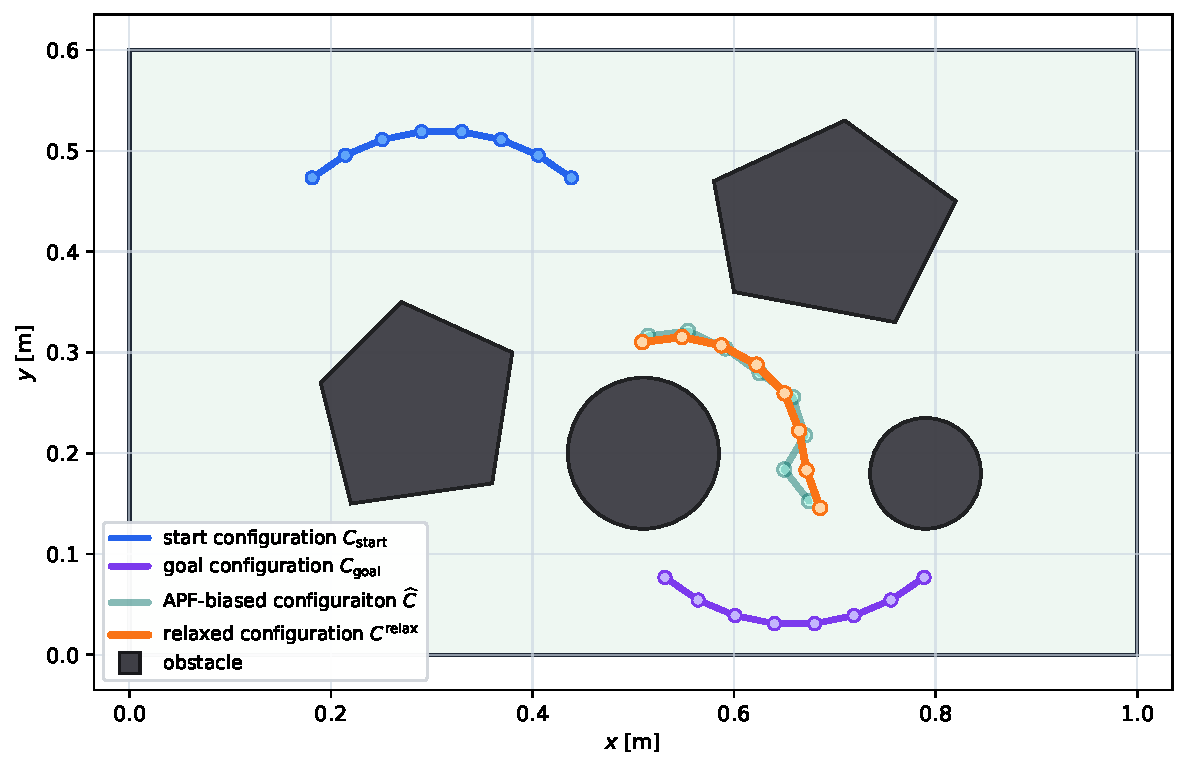
\includegraphics[width=0.8\linewidth]{figures/config_apf_pipeline_step_relaxation.pdf}
%     \caption{Projected elastic relaxation of an APF-biased cable configuration.
%     The relaxed configuration remains close to the APF-biased sample while
%     improving obstacle clearance and satisfying local segment-deviation
%     constraints.}
%     \label{fig:relaxation}
% \end{figure}


\subsection{Cable Elastic Relaxation}
\label{subsec:gcr_constrained_relaxation}

The projected elastic relaxation step transforms the APF-biased configuration
\(\widehat{C}\) into a corrected candidate
\[
C^{\mathrm{relax}}
=
(p_1^{\mathrm{relax}},p_2^{\mathrm{relax}},\ldots,p_N^{\mathrm{relax}})
\]
that remains close to \(\widehat{C}\) while preserving the local shape of a nearby feasible reference configuration \(C^{\mathrm{ref}}\).

Let \(C=(p_1,p_2,\ldots,p_N)\) be the configuration optimized during
relaxation. The relaxation objective is defined as
% \begin{equation}
% \begin{aligned}
% \Phi(C)
% =
% &
% \lambda_{\text{apf}}
% \sum_{n=1}^{N}
% \left\|
% p_n-\widehat{p}_n
% \right\|^2
% +
% \lambda_{\text{s}}
% \sum_{k=1}^{N-1}
% \left\|
% v_k(C)-v_k^{\mathrm{ref}}
% \right\|^2
% \\
% &
% +
% \lambda_{\text{b}}
% \sum_{k=1}^{N-2}
% \left\|
% \Delta^2 p_k-\Delta^2 p_k^{\mathrm{ref}}
% \right\|^2 ,
% \end{aligned}
% \label{eq:relaxation_objective}
% \end{equation}
\begin{equation}
\Phi(C)
=
\lambda_{\mathrm{apf}}
\sum_{n=1}^{N}
\left\|
p_n-\widehat{p}_n
\right\|^2
+
E_{\mathrm{def}}(C,C^{\mathrm{ref}})
\label{eq:relaxation_objective}
\end{equation}
% where
% \begin{equation}
% v_k(C)=p_{k+1}-p_k,
% \qquad
% v_k^{\mathrm{ref}}=p_{k+1}^{\mathrm{ref}}-p_k^{\mathrm{ref}},
% \label{eq:relaxation_segment_vectors}
% \end{equation}
% and
% \begin{equation}
% \Delta^2 p_k=p_{k+2}-2p_{k+1}+p_k .
% \label{eq:relaxation_second_difference}
% \end{equation}
The first term keeps the relaxed configuration close to the APF-biased configuration. The deformation term \(E_{\mathrm{def}}(C,C^{\mathrm{ref}})\) contains the segment-vector and discrete-curvature penalties defined in \eqref{eq:gcr_transition_deformation_energy}; these terms reduce excessive stretching, compression, local rotation, and abrupt bending relative to the reference configuration. The weight \(\lambda_{\mathrm{apf}}>0\) controls the relative influence of tracking the APF-biased sample.

The relaxation is initialized from the APF-biased configuration:
\begin{equation}
C^0=\widehat{C}.
\label{eq:relaxation_initial_condition}
\end{equation}
At iteration \(m\), a gradient step is first applied:
\begin{equation}
C^{m+\frac{1}{2}}
=
C^m
-
h_{\mathrm{relax}}
\nabla \Phi(C^m),
\label{eq:relaxation_gradient_step}
\end{equation}
where \(h_{\mathrm{relax}}>0\) is the relaxation step size.

The intermediate configuration is then corrected by a sequence of projection
operators:
\begin{equation}
C^{m+1}
=
\Pi_{\mathrm{end}}
\Pi_{\mathcal{W}}
\Pi_{\delta}
\Pi_{\mathrm{obs}}
\left(
C^{m+\frac{1}{2}}
\right).
\label{eq:relaxation_projection_step}
\end{equation}
% The operators are applied from right to left. 
Each projection has a specific role. The obstacle projection \(\Pi_{\mathrm{obs}}\) pushes cable samples away from obstacles when the required clearance is violated. The segment-deviation projection \(\Pi_{\delta}\) enforces an upper bound on local deformation with respect to the reference shape. The workspace projection \(\Pi_{\mathcal{W}}\) keeps all cable nodes inside the bounded planning workspace. Finally, the endpoint projection \(\Pi_{\mathrm{end}}\) restores the APF-updated endpoint positions, so that only the internal cable nodes are modified by the relaxation process.

Obstacle clearance is evaluated at sampled points along each cable segment:
\begin{equation}
x_{kq}(C)
=
(1-\rho_q)p_k+\rho_q p_{k+1},
\qquad
\rho_q=\frac{q}{Q},
\qquad
q=0,\ldots,Q .
\label{eq:relaxation_sampled_points}
\end{equation}
The clearance condition is
\begin{equation}
d_{\mathcal{O}}\bigl(x_{kq}(C)\bigr)
\geq
d_{\mathrm{safe}},
\label{eq:relaxation_clearance_constraint}
\end{equation}
where \(d_{\mathcal{O}}(\cdot)\) is the signed obstacle distance and
\(d_{\mathrm{safe}}>0\) is the required safety margin. If a sampled point
violates this condition, \(\Pi_{\mathrm{obs}}\) applies a local correction in
the outward obstacle-normal direction. This correction is distributed to the
two points of the corresponding cable segment. Thus, the projection improves
clearance without globally reshaping the entire cable.

The segment-deviation projection limits the change of each local segment vector
relative to the reference configuration. For each segment, the admissible
deviation is
\begin{equation}
\left\|
\bigl(p_{k+1}-p_k\bigr)
-
\bigl(p_{k+1}^{\mathrm{ref}}-p_k^{\mathrm{ref}}\bigr)
\right\|
\leq
\delta_{\ell},
\qquad
k=1,\ldots,N-1 ,
\label{eq:relaxation_segment_constraint}
\end{equation}
where \(\delta_{\ell}>0\) is the maximum allowed segment-vector deviation. If
this bound is exceeded, \(\Pi_{\delta}\) shortens the deviation vector to the
radius \(\delta_{\ell}\) and updates the corresponding segment nodes
accordingly.

% This projection is not redundant with the segment-preservation term in
% \eqref{eq:relaxation_objective}. The objective term is a soft  regularization term: it penalizes deformation but does not strictly prevent the optimizer from exceeding the admissible deformation limit, especially when the tracking term or obstacle-clearance correction dominates. In contrast, \(\Pi_{\delta}\) enforces a hard feasibility constraint. Therefore, the objective encourages physically reasonable relaxation, while the projection guarantees that the relaxed candidate satisfies the local deformation bound required by the planner.

The workspace projection enforces the rectangular workspace bounds
\[
\mathcal{W}
=
[x_{\min},x_{\max}]
\times
[y_{\min},y_{\max}] .
\]
For a point \(p_n=(x_n,y_n)\), this projection clips the coordinates to the
workspace limits:
\begin{equation}
\Pi_{\mathcal{W}}(p_n)
=
\left(
\operatorname{clip}(x_n,x_{\min},x_{\max}),
\operatorname{clip}(y_n,y_{\min},y_{\max})
\right),
\label{eq:relaxation_workspace_projection}
\end{equation}
where
\begin{equation}
\operatorname{clip}(a,a_{\min},a_{\max})
=
\min
\left\{
a_{\max},
\max\{a_{\min},a\}
\right\}
\label{eq:relaxation_clip_operator}
\end{equation}

The endpoint projection \(\Pi_{\mathrm{end}}\) fixes the two cable endpoints:
\begin{equation}
p_1=\widehat{p}_1,
\qquad
p_N=\widehat{p}_N
\label{eq:relaxation_endpoint_constraint}
\end{equation}

After \(M_{\mathrm{relax}}\) iterations, the relaxed configuration is defined as
\begin{equation}
C^{\mathrm{relax}}=C^{M_{\mathrm{relax}}}.
\label{eq:relaxed_configuration_result}
\end{equation}
The resulting candidate \(C^{\mathrm{relax}}\) is considered for insertion into the search tree only if it passes the final admissibility check with respect to the reference configuration,
\begin{equation}
C^{\mathrm{relax}}\in\mathcal{C}_{\mathrm{free}}(C^{\mathrm{ref}}).
\label{eq:relaxed_static_validation}
\end{equation}
This check verifies workspace bounds, segment-deviation limits, and collision
freedom of all cable segments.

The effect of the relaxation step is illustrated in
Fig.~\ref{fig:relaxation}.

\begin{figure}[h]
    \centering
    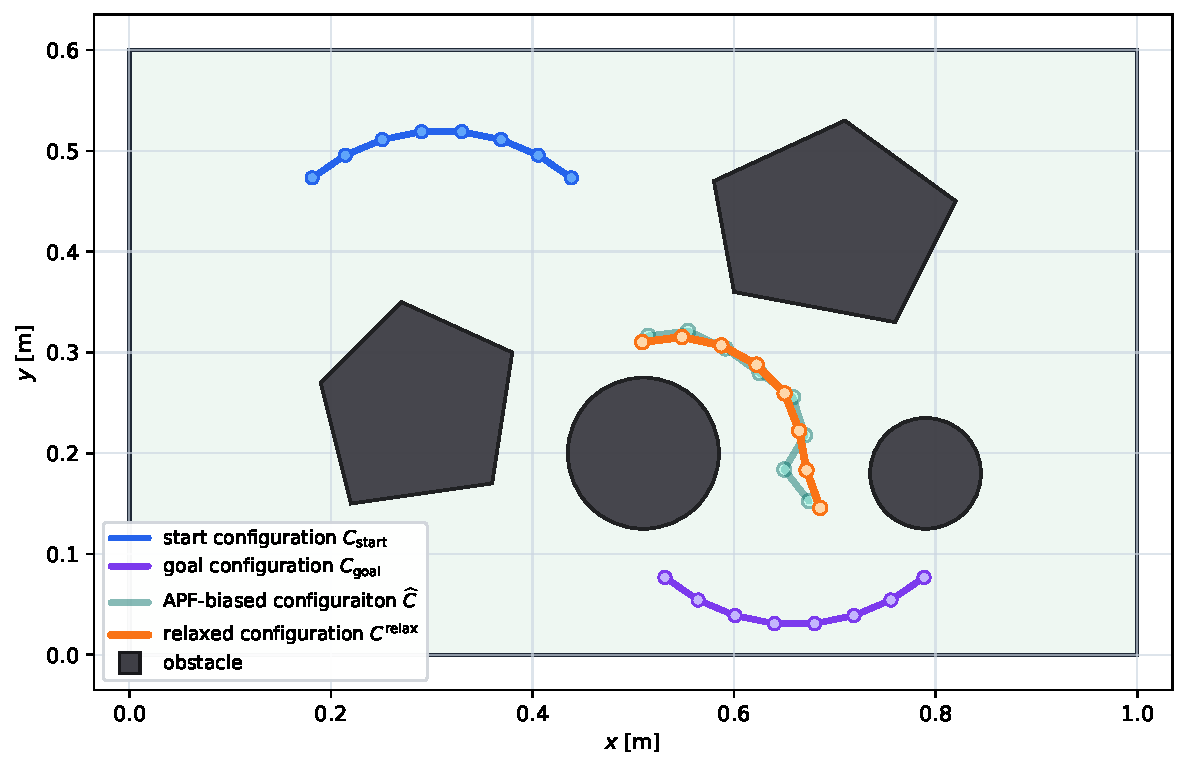
\includegraphics[width=0.8\linewidth]{figures/config_apf_pipeline_step_relaxation.pdf}
    \caption{Projected elastic relaxation of an APF-biased cable configuration.
    The relaxed configuration remains close to the APF-biased sample while
    improving obstacle clearance and satisfying local segment-deviation
    constraints.}
    \label{fig:relaxation}
\end{figure}


% ------------------------------------------------------------
% \subsection{Feasible Parent Selection and Node Insertion}
% \label{subsec:gcr_parent_selection}

% After the relaxed configuration \(C^{\mathrm{relax}}\) has passed the static admissibility check in \ref{eq:relaxed_static_validation}, the planner searches for a feasible parent in the active tree. The parent selection step determines whether the relaxed configuration can
% be connected to an existing tree vertex by a collision-free local deformation.

% Let \(V_{\mathrm{act}}\) denote the set of vertices in the active tree. A vertex \(C_i\in V_{\mathrm{act}}\) is first considered as a parent candidate only if it lies within the local connection radius:
% \begin{equation}
% d(C_i,C^{\mathrm{relax}})
% \leq
% \epsilon 
% \label{eq:parent_distance_filter}
% \end{equation}
% This condition restricts the parent search to nearby configurations and avoids large local deformations that may be difficult to validate. The set of nearby parent candidates is therefore
% \begin{equation}
% \mathcal{V}_{\epsilon}
% =
% \left\{
% C_i\in V_{\mathrm{act}}
% \ \middle|\
% d(C_i,C^{\mathrm{relax}})\leq\epsilon
% \right\}
% \label{eq:nearby_parent_set}
% \end{equation}
% The candidates in \(\mathcal{V}_{\epsilon}\) are ordered according to their distance from \(C^{\mathrm{relax}}\). Only a bounded number of nearest candidates is evaluated. This keeps the parent-selection step local and computationally bounded.

% Distance proximity alone is not sufficient for parent selection. A candidate parent must also produce a deformation-feasible edge. For each candidate \(C_i\), the swept envelope between \(C_i\) and \(C^{\mathrm{relax}}\) is constructed as
% \begin{equation}
% \mathcal{E}_{i,\mathrm{relax}}
% =
% \operatorname{Poly}
% \left(
% p_1^{i},p_2^{i},\ldots,p_N^{i},
% p_N^{\mathrm{relax}},p_{N-1}^{\mathrm{relax}},
% \ldots,p_1^{\mathrm{relax}}
% \right).
% \label{eq:parent_swept_envelope}
% \end{equation}
% The candidate parent is feasible only if this swept envelope does not intersect
% the obstacle region:
% \begin{equation}
% \mathcal{E}_{i,\mathrm{relax}}
% \cap
% \mathcal{O}
% =
% \emptyset .
% \label{eq:parent_swept_envelope_free}
% \end{equation}
% Equivalently, the transition-validity condition is written as
% \begin{equation}
% \chi_{\mathrm{sw}}
% \left(
% C_i,C^{\mathrm{relax}}
% \right)
% =
% 1 
% \label{eq:parent_swept_clear_check}
% \end{equation}

% The feasible parent set is then defined as
% \begin{equation}
% \mathcal{V}_{\mathrm{par}}
% =
% \left\{
% C_i\in \mathcal{V}_{\epsilon}
% \ \middle|\
% \chi_{\mathrm{sw}}
% \left(
% C_i,C^{\mathrm{relax}}
% \right)
% =1
% \right\}.
% \label{eq:feasible_parent_set}
% \end{equation}
% If \(\mathcal{V}_{\mathrm{par}}=\emptyset\), the relaxed configuration is rejected because no valid local deformation connects it to the active tree.

% If at least one feasible parent exists, the nearest feasible parent is selected:
% \begin{equation}
% C^{\mathrm{par}}
% =
% \arg\min_{C_i\in\mathcal{V}_{\mathrm{par}}}
% d(C_i,C^{\mathrm{relax}}).
% \label{eq:selected_parent_nearest}
% \end{equation}
% The relaxed configuration is then inserted into the active tree as a new vertex:
% \begin{equation}
% C^{\mathrm{new}}
% =
% C^{\mathrm{relax}}.
% \label{eq:new_node_is_relaxed}
% \end{equation}
% The corresponding edge
% \begin{equation}
% \left(
% C^{\mathrm{par}},C^{\mathrm{new}}
% \right)
% \label{eq:new_tree_edge}
% \end{equation}
% is added to the active tree, and the parent pointer of \(C^{\mathrm{new}}\) is
% set to \(C^{\mathrm{par}}\).

% The two possible outcomes of the parent-selection test are illustrated in
% Fig.~\ref{fig:polygon}. In Fig.~\ref{fig:polygon_free}, the swept corridor
% between the candidate parent and the relaxed configuration is obstacle-free.
% Therefore, the candidate parent is accepted and the relaxed configuration can be
% inserted into the active tree. In Fig.~\ref{fig:polygon_blocked}, the swept
% corridor intersects an obstacle. Although the two endpoint configurations may be
% individually valid, the deformation between them is not collision-free, and the
% candidate parent is rejected.

% \begin{figure}[h]
%     \centering
%     \subfloat[Feasible parent connection. The swept corridor between the
%     candidate parent \(C^{\mathrm{cand.parent}}\) and the relaxed configuration
%     \(C^{\mathrm{relax}}\) is obstacle-free.
%     \label{fig:polygon_free}]{
%     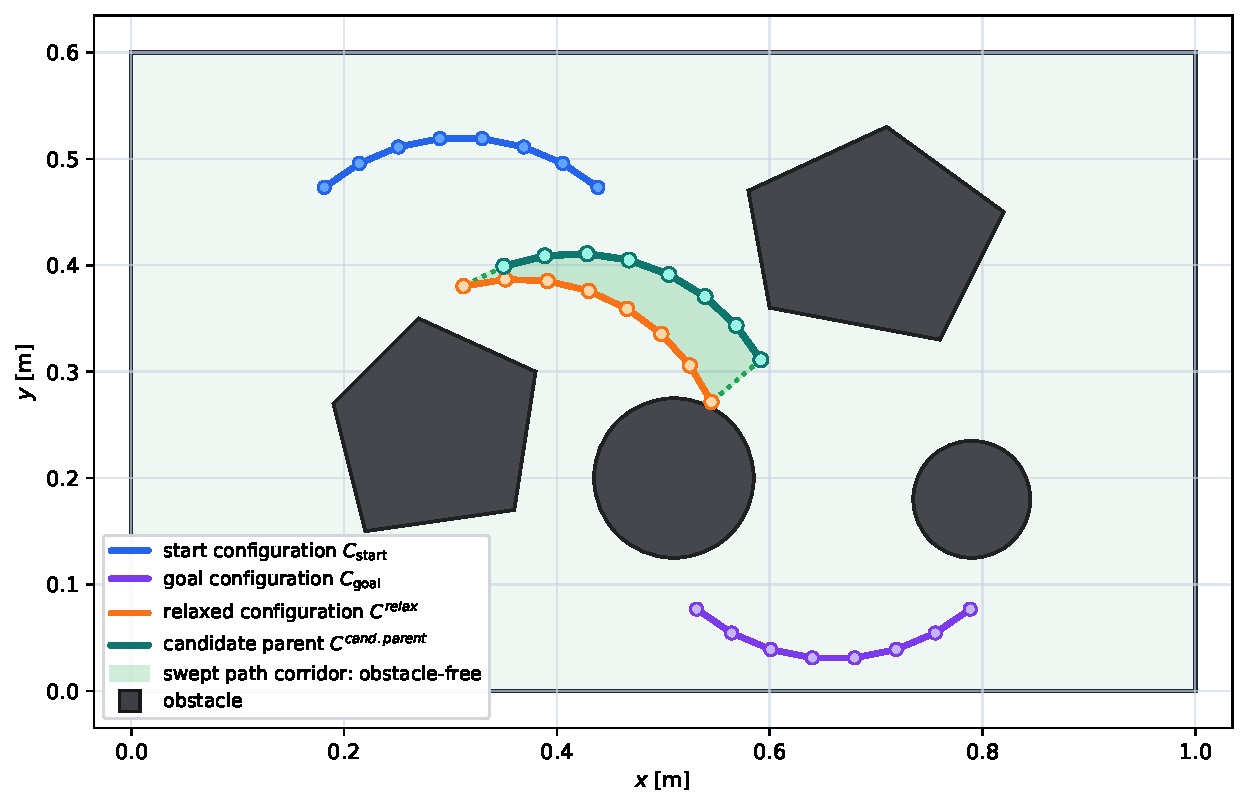
\includegraphics[width=0.75\linewidth]{figures/connection_polygon_case_free.pdf}}
%     \\
%     \subfloat[Rejected parent connection. The swept corridor intersects an
%     obstacle, so the transition from the candidate parent to
%     \(C^{\mathrm{relax}}\) is not swept-clear.
%     \label{fig:polygon_blocked}]{
%     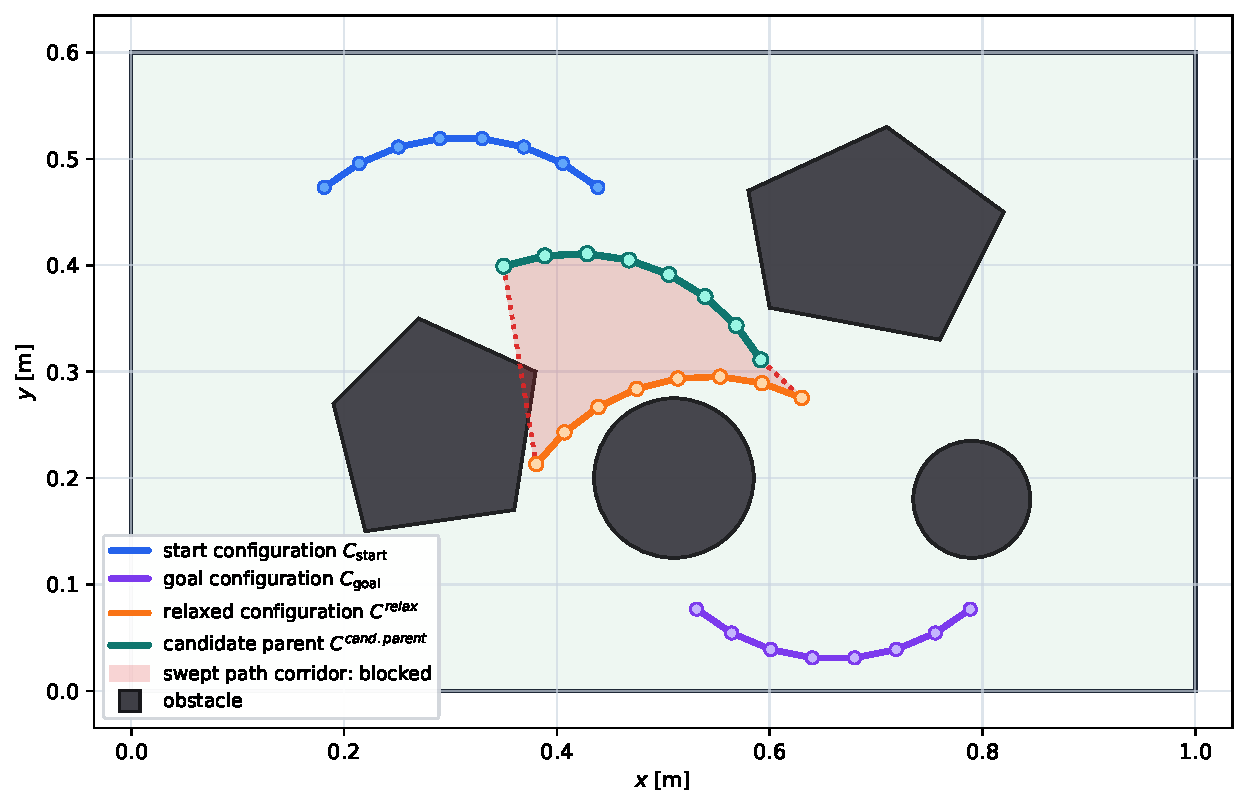
\includegraphics[width=0.75\linewidth]{figures/connection_polygon_case_blocked.pdf}}
%     \caption{Feasible parent selection using the swept envelope between a
%     candidate parent configuration and the relaxed configuration. The relaxed
%     configuration can be inserted into the active tree only if at least one
%     nearby parent produces an obstacle-free swept corridor.}
%     \label{fig:polygon}
% \end{figure}

\subsection{Feasible Parent Selection and Node Insertion}
\label{subsec:gcr_parent_selection}

After the relaxed configuration \(C^{\mathrm{relax}}\) has passed the static
admissibility check in \eqref{eq:relaxed_static_validation}, the planner searches
for a feasible parent in the active tree. The parent selection step determines
whether the relaxed configuration can be connected to an existing tree vertex by
a collision-free and endpoint-consistent local deformation.

In contrast to static configuration validation, local transition validation
depends on the ordering of the cable nodes. The planner therefore considers
both ordered representatives of the relaxed configuration,
\(\left(C^{\mathrm{relax}}\right)^{\sigma}\) with \(\sigma\in\{+1,-1\}\),
following the endpoint-order notation of
Section~\ref{subsec:ordered_transition_feasibility}. Each vertex already stored
in the active tree has a fixed endpoint ordering, because it was inserted
through a previously validated ordered transition.

Let \(V_{\mathrm{act}}\) denote the set of vertices in the active tree. A pair
\(\left(C_i,\sigma\right)\), where \(C_i\in V_{\mathrm{act}}\) and
\(\sigma\in\{+1,-1\}\), is first considered as a parent-candidate pair only if
the corresponding ordered relaxed configuration lies within the local connection
radius:
\begin{equation}
d
\left(
C_i,
\left(C^{\mathrm{relax}}\right)^{\sigma}
\right)
\leq
\epsilon .
\label{eq:parent_distance_filter}
\end{equation}
This condition restricts the parent search to nearby configurations and avoids
large local deformations that may be difficult to validate. The set of nearby
parent-candidate pairs is therefore
\begin{equation}
\mathcal{V}_{\epsilon}
=
\left\{
\left(C_i,\sigma\right)
\ \middle|\
C_i\in V_{\mathrm{act}},
\;
\sigma\in\{+1,-1\},
\;
d
\left(
C_i,
\left(C^{\mathrm{relax}}\right)^{\sigma}
\right)
\leq
\epsilon
\right\}.
\label{eq:nearby_parent_set}
\end{equation}
The candidates in \(\mathcal{V}_{\epsilon}\) are ordered according to their
distance from the corresponding ordered relaxed configuration, and only a
bounded number of nearest candidates is evaluated.

Distance proximity alone is not sufficient for parent selection. A candidate
parent must also produce a deformation-feasible edge under the selected endpoint
ordering. For each candidate pair \(\left(C_i,\sigma\right)\), let
\[
\left(C^{\mathrm{relax}}\right)^{\sigma}
=
\left(
p_1^{\mathrm{relax},\sigma},
p_2^{\mathrm{relax},\sigma},
\ldots,
p_N^{\mathrm{relax},\sigma}
\right).
\]
The swept envelope between \(C_i\) and
\(\left(C^{\mathrm{relax}}\right)^{\sigma}\) is constructed as
\begin{equation}
\mathcal{E}_{i,\mathrm{relax}}^{\sigma}
=
\bigcup_{k=1}^{N-1}
\operatorname{conv}
\left\{
p_k^{i},
p_{k+1}^{i},
p_{k+1}^{\mathrm{relax},\sigma},
p_k^{\mathrm{relax},\sigma}
\right\}.
\label{eq:parent_swept_envelope}
\end{equation}
The candidate parent is feasible only if this swept envelope does not intersect
the obstacle region:
\begin{equation}
\mathcal{E}_{i,\mathrm{relax}}^{\sigma}
\cap
\mathcal{O}
=
\emptyset .
\label{eq:parent_swept_envelope_free}
\end{equation}
Equivalently, the swept-clear condition is written as
\begin{equation}
\chi_{\mathrm{sw}}
\left(
C_i,
\left(C^{\mathrm{relax}}\right)^{\sigma}
\right)
=
1 .
\label{eq:parent_swept_clear_check}
\end{equation}

As established in Section~\ref{subsec:ordered_transition_feasibility},
\(\chi_{\mathrm{sw}}\) is not invariant under reversal of a single
configuration, so the parent-selection step evaluates the swept-envelope
condition for the actual ordered representative that would be inserted into the
tree. To include ordered edge-feasibility consistency in the same
edge-validation step, the full ordered transition predicate
\(\Gamma(\cdot,\cdot)\) of \eqref{eq:ordered_edge_feasibility_predicate} is
used. Thus, the feasible parent set is defined as
\begin{equation}
\mathcal{V}_{\mathrm{par}}
=
\left\{
\left(C_i,\sigma\right)\in \mathcal{V}_{\epsilon}
\ \middle|\
\Gamma
\left(
C_i,
\left(C^{\mathrm{relax}}\right)^{\sigma}
\right)
=
1
\right\}.
\label{eq:feasible_parent_set}
\end{equation}
In particular,
\begin{equation}
\Gamma
\left(
C_i,
\left(C^{\mathrm{relax}}\right)^{\sigma}
\right)
=
1
\
\Longrightarrow
\
\chi_{\mathrm{sw}}
\left(
C_i,
\left(C^{\mathrm{relax}}\right)^{\sigma}
\right)
=
1 .
\label{eq:gamma_implies_swept_clear_parent}
\end{equation}

If \(\mathcal{V}_{\mathrm{par}}=\emptyset\), the relaxed configuration is
rejected because no valid ordered local deformation connects it to the active
tree.

If at least one feasible parent exists, the parent and the ordering of the
relaxed configuration are selected from \(\mathcal{V}_{\mathrm{par}}\) by
minimizing the resulting cost-to-come. Thus, the selected pair is
\begin{equation}
\begin{aligned}
\left(
C^{\mathrm{par}},
\sigma^{\ast}
\right)
&=
\arg\min_{\left(C_i,\sigma\right)\in\mathcal{V}_{\mathrm{par}}}
\Bigl[
g(C_i)
+
d
\left(
C_i,
\left(C^{\mathrm{relax}}\right)^{\sigma}
\right)
\\
&\quad+
\alpha_{\mathrm{def}}
E_{\mathrm{def}}
\left(
\left(C^{\mathrm{relax}}\right)^{\sigma},
C_i
\right)
\Bigr].
\end{aligned}
\label{eq:selected_parent_cost}
\end{equation}
The relaxed configuration is then inserted into the active tree using the
selected endpoint ordering:
\begin{equation}
C^{\mathrm{new}}
=
\left(C^{\mathrm{relax}}\right)^{\sigma^{\ast}}.
\label{eq:new_node_is_relaxed}
\end{equation}
The corresponding edge
\begin{equation}
\left(
C^{\mathrm{par}},C^{\mathrm{new}}
\right)
\label{eq:new_tree_edge}
\end{equation}
is added to the active tree, and the parent pointer of \(C^{\mathrm{new}}\) is
set to \(C^{\mathrm{par}}\).

By construction, every inserted edge satisfies
\(\Gamma(C^{\mathrm{par}},C^{\mathrm{new}})=1\) and hence, by
\eqref{eq:gamma_implies_swept_clear_parent}, represents an obstacle-free swept
deformation under the selected endpoint correspondence. This prevents a
configuration from being accepted under one endpoint ordering and later
reinterpreted using another ordering that was not validated during planning.

The two possible outcomes of the parent-selection test are illustrated in
Fig.~\ref{fig:polygon}. In Fig.~\ref{fig:polygon_free}, the swept corridor
between the candidate parent and the ordered relaxed configuration is
obstacle-free. Therefore, the candidate parent is accepted and the ordered
relaxed configuration can be inserted into the active tree. In
Fig.~\ref{fig:polygon_blocked}, the swept corridor intersects an obstacle.
Although the two endpoint configurations may be individually valid, the ordered
deformation between them is not collision-free, and the candidate parent is
rejected.

\begin{figure}[h]
    \centering
    \subfloat[Feasible parent connection. The swept corridor between the
    candidate parent \(C^{\mathrm{cand.parent}}\) and the ordered relaxed
    configuration \(C^{\mathrm{new}}\) is obstacle-free.
    \label{fig:polygon_free}]{
    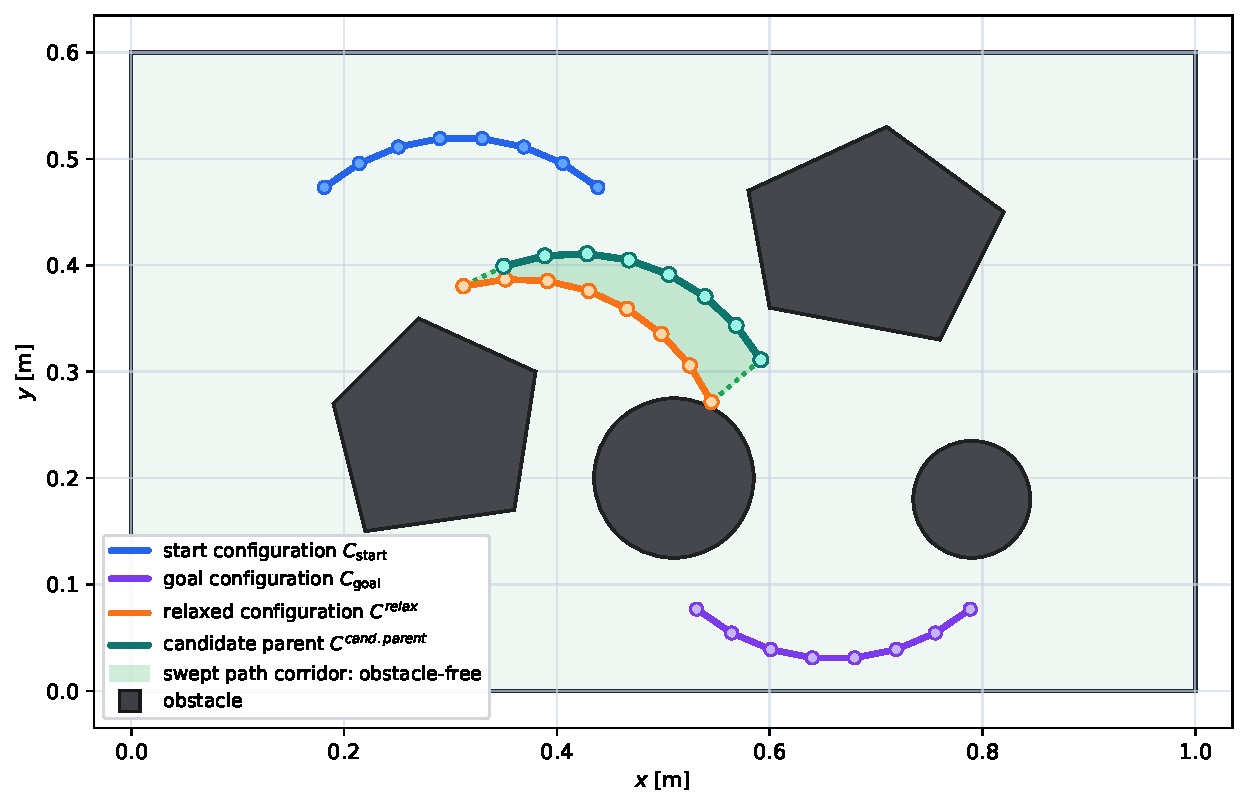
\includegraphics[width=0.75\linewidth]{figures/connection_polygon_case_free.pdf}}
    \\
    \subfloat[Rejected parent connection. The swept corridor intersects an
    obstacle, so the transition from the candidate parent to the ordered relaxed
    configuration is not swept-clear.
    \label{fig:polygon_blocked}]{
    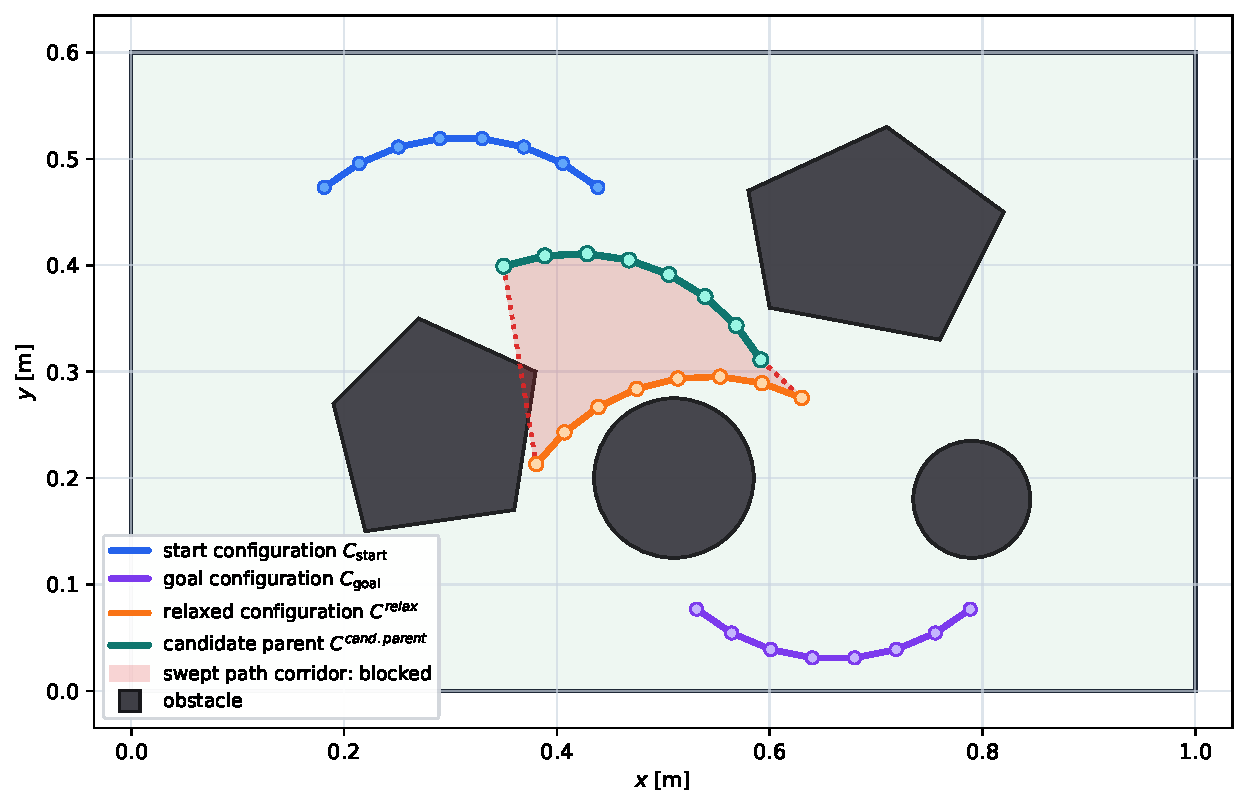
\includegraphics[width=0.75\linewidth]{figures/connection_polygon_case_blocked.pdf}}
    \caption{Feasible parent selection using the swept envelope between a
    candidate parent configuration and the ordered relaxed configuration. The
    relaxed configuration can be inserted into the active tree only if at least
    one nearby parent produces an obstacle-free and endpoint-consistent swept
    corridor.}
    \label{fig:polygon}
\end{figure}



% Thus, node insertion requires both static admissibility of
% \(C^{\mathrm{relax}}\) and transition feasibility from an existing tree vertex. This prevents the planner from adding configurations that are individually collision-free but cannot be reached through a valid local cable deformation.

% ------------------------------------------------------------
% \subsection{Tree Connection and Path Extraction}
% \label{subsec:gcr_tree_connection}


% After a new node (configuration) has been inserted into the active tree, the algorithm attempts to connect it to the opposite tree. Let $V_{\mathrm{opp}}$ denote the vertex set of the opposite tree. The nearest candidate connection node is
% \begin{equation}
% C_{\mathrm{conn}}
% =
% \underset{C\in V_{\mathrm{opp}}}{\arg\min} \
% d(C,C^{\mathrm{new}}).
% \label{eq:gcr_connection_candidate}
% \end{equation}

% A valid connection is found if the two meeting configurations are sufficiently close and the deformation between them is swept-clear:
% \begin{equation}
% d(C^{\mathrm{new}},C_{\mathrm{conn}})
% \leq
% \epsilon,
% \label{eq:gcr_connection_distance_condition}
% \end{equation}
% and
% \begin{equation}
% \chi_{\mathrm{sw}}(C^{\mathrm{new}},C_{\mathrm{conn}})=1
% \label{eq:gcr_connection_swept_clear_condition}
% \end{equation}

% If the active tree is $T_{\mathrm{s}}$, the meeting nodes are assigned as
% \begin{equation}
% C_{\mathrm{meet}}^{\mathrm{s}}
% =
% C^{\mathrm{new}},
% \qquad
% C_{\mathrm{meet}}^{\mathrm{g}}
% =
% C_{\mathrm{conn}}
% \label{eq:gcr_meeting_nodes_start_active}
% \end{equation}
% If the active tree is $T_{\mathrm{g}}$, the assignment is
% \begin{equation}
% C_{\mathrm{meet}}^{\mathrm{s}}
% =
% C_{\mathrm{conn}},
% \qquad
% C_{\mathrm{meet}}^{\mathrm{g}}
% =
% C^{\mathrm{new}}
% \label{eq:gcr_meeting_nodes_goal_active}
% \end{equation}

% The start-side partial path is obtained by tracing parent pointers from $C_{\mathrm{meet}}^{\mathrm{s}}$ to the root $C_{\mathrm{start}}$ and reversing the order:
% \begin{equation}
% \mathcal{P}_{\mathrm{s}}
% =
% \mathrm{Reverse}
% \left(
% \mathrm{TraceParents}
% \left(
% C_{\mathrm{meet}}^{\mathrm{s}}
% \rightarrow
% C_{\mathrm{start}}
% \right)
% \right)
% \label{eq:gcr_start_side_path}
% \end{equation}
% The goal-side partial path is obtained by tracing parent pointers from $C_{\mathrm{meet}}^{\mathrm{g}}$ to the root $C_{\mathrm{goal}}$:
% \begin{equation}
% \mathcal{P}_{\mathrm{g}}
% =
% \mathrm{TraceParents}
% \left(
% C_{\mathrm{meet}}^{\mathrm{g}}
% \rightarrow
% C_{\mathrm{goal}}
% \right)
% \label{eq:gcr_goal_side_path}
% \end{equation}
% Thus, the complete solution path is then
% \begin{equation}
% \mathcal{P}
% =
% \mathcal{P}_{\mathrm{s}}
% \oplus
% \mathcal{P}_{\mathrm{g}},
% \label{eq:gcr_complete_path_concatenation}
% \end{equation}
% where $\oplus$ denotes path concatenation. By construction, every configuration in $\mathcal{P}$ belongs to $\mathcal{C}_{\mathrm{free}}$, and every edge between consecutive configurations satisfies the deformation-feasibility condition.

\subsection{Tree Connection and Path Extraction}
\label{subsec:gcr_tree_connection}

After a new node \(C^{\mathrm{new}}\) has been inserted into the active tree,
the algorithm attempts to connect it to the opposite tree. Since each tree vertex
is stored with a fixed endpoint ordering, the connection step must evaluate the
ordered transition between the two meeting configurations. Therefore, the
connection between the two trees is validated using the same ordered
edge-feasibility predicate \(\Gamma(\cdot,\cdot)\) used in the parent-selection
stage.

Let \(V_{\mathrm{opp}}\) denote the vertex set of the opposite tree. The nearest
candidate connection node is first defined as
\begin{equation}
C_{\mathrm{conn}}
=
\underset{C\in V_{\mathrm{opp}}}{\arg\min} \
d(C,C^{\mathrm{new}}).
\label{eq:gcr_connection_candidate}
\end{equation}
This nearest-neighbor query provides a candidate connection between the two
trees. However, distance proximity alone is not sufficient: the connection edge
is traversed in the direction of the final path, from \(C^{\mathrm{new}}\) to
\(C_{\mathrm{conn}}\) when the active tree is \(T_{\mathrm{s}}\), and from
\(C_{\mathrm{conn}}\) to \(C^{\mathrm{new}}\) when the active tree is
\(T_{\mathrm{g}}\). The ordered transition in this direction must lie within
the connection radius \(\epsilon\) and satisfy the ordered edge-feasibility
predicate \(\Gamma(\cdot,\cdot)\); otherwise, an invalid endpoint
correspondence could generate a swept envelope that collides during the
connection transition even though both meeting configurations are individually
collision-free.

If the nearest candidate \(C_{\mathrm{conn}}\) does not satisfy the ordered
connection condition, the planner may evaluate a bounded set of nearby vertices
from \(V_{\mathrm{opp}}\). This set is defined as
\begin{equation}
\mathcal{V}_{\mathrm{conn}}
=
\left\{
C_j\in V_{\mathrm{opp}}
\ \middle|\
d(C_j,C^{\mathrm{new}})\leq\epsilon
\right\}.
\label{eq:gcr_connection_candidate_set}
\end{equation}
When the active tree is \(T_{\mathrm{s}}\), the feasible connection set is
\begin{equation}
\mathcal{V}_{\mathrm{conn}}^{\mathrm{feas}}
=
\left\{
C_j\in \mathcal{V}_{\mathrm{conn}}
\ \middle|\
\Gamma(C^{\mathrm{new}},C_j)=1
\right\}.
\label{eq:gcr_feasible_connection_set_start_active}
\end{equation}
When the active tree is \(T_{\mathrm{g}}\), the feasible connection set is
\begin{equation}
\mathcal{V}_{\mathrm{conn}}^{\mathrm{feas}}
=
\left\{
C_j\in \mathcal{V}_{\mathrm{conn}}
\ \middle|\
\Gamma(C_j,C^{\mathrm{new}})=1
\right\}.
\label{eq:gcr_feasible_connection_set_goal_active}
\end{equation}
If
\begin{equation}
\mathcal{V}_{\mathrm{conn}}^{\mathrm{feas}}=\emptyset,
\end{equation}
then no valid tree connection is made during the current iteration. Otherwise,
the connection node is selected as the nearest feasible connection candidate:
\begin{equation}
C_{\mathrm{conn}}
=
\underset{C_j\in \mathcal{V}_{\mathrm{conn}}^{\mathrm{feas}}}{\arg\min} \
d(C_j,C^{\mathrm{new}}).
\label{eq:gcr_selected_feasible_connection}
\end{equation}

If the active tree is \(T_{\mathrm{s}}\), the meeting nodes are assigned as
\begin{equation}
C_{\mathrm{meet}}^{\mathrm{s}}
=
C^{\mathrm{new}},
\qquad
C_{\mathrm{meet}}^{\mathrm{g}}
=
C_{\mathrm{conn}}.
\label{eq:gcr_meeting_nodes_start_active}
\end{equation}
If the active tree is \(T_{\mathrm{g}}\), the assignment is
\begin{equation}
C_{\mathrm{meet}}^{\mathrm{s}}
=
C_{\mathrm{conn}},
\qquad
C_{\mathrm{meet}}^{\mathrm{g}}
=
C^{\mathrm{new}}.
\label{eq:gcr_meeting_nodes_goal_active}
\end{equation}

The start-side partial path is obtained by tracing parent pointers from
\(C_{\mathrm{meet}}^{\mathrm{s}}\) to the root \(C_{\mathrm{start}}\) and
reversing the order:
\begin{equation}
\mathcal{P}_{\mathrm{s}}
=
\mathrm{Reverse}
\left(
\mathrm{TraceParents}
\left(
C_{\mathrm{meet}}^{\mathrm{s}}
\rightarrow
C_{\mathrm{start}}
\right)
\right).
\label{eq:gcr_start_side_path}
\end{equation}
The goal-side partial path is obtained by tracing parent pointers from
\(C_{\mathrm{meet}}^{\mathrm{g}}\) to the root \(C_{\mathrm{goal}}\):
\begin{equation}
\mathcal{P}_{\mathrm{g}}
=
\mathrm{TraceParents}
\left(
C_{\mathrm{meet}}^{\mathrm{g}}
\rightarrow
C_{\mathrm{goal}}
\right).
\label{eq:gcr_goal_side_path}
\end{equation}
Thus, the complete solution path is
\begin{equation}
\mathcal{P}
=
\mathcal{P}_{\mathrm{s}}
\oplus
\mathcal{P}_{\mathrm{g}},
\label{eq:gcr_complete_path_concatenation}
\end{equation}
where \(\oplus\) denotes path concatenation.

By construction, every configuration in \(\mathcal{P}\) belongs to
\(\mathcal{C}_{\mathrm{free}}\), and every edge between consecutive
configurations satisfies the ordered deformation-feasibility condition:
\begin{equation}
\Gamma(C_k,C_{k+1})=1,
\qquad
k=0,\ldots,|\mathcal{P}|-2.
\label{eq:gcr_complete_path_ordered_feasibility}
\end{equation}
Consequently,
\begin{equation}
\chi_{\mathrm{sw}}(C_k,C_{k+1})=1,
\qquad
k=0,\ldots,|\mathcal{P}|-2.
\label{eq:gcr_complete_path_swept_clear_feasibility}
\end{equation}

% CHECK 5.7
\subsection{Post-Connection Shortcut Refinement}
\label{subsec:gcr_shortcut_refinement}

The first path obtained by connecting the two trees may contain unnecessary intermediate configurations. Therefore, after a feasible solution has been found, a shortcut-based refinement step is applied to reduce the number of cable configurations in the path.
% The assignment between ordered cable endpoints and robot end-effectors is handled afterward in the endpoint-ordering and execution-validation stage described in Section~\ref{subsec:gcr_path_refinement}.

Let the initial connected path be
\begin{equation}
\mathcal{P}^{0}
=
\left\{
C_0,C_1,\ldots,C_K
\right\},
\qquad
C_0=C_{\mathrm{start}},
\qquad
C_K=C_{\mathrm{goal}}
\label{eq:gcr_initial_solution_path}
\end{equation}
For any pair of configurations $C_i$ and $C_j$ with $j>i+1$, the algorithm attempts to replace the subsequence
\begin{equation}
\left(
C_i,C_{i+1},\ldots,C_j
\right)
\label{eq:gcr_shortcut_subsequence}
\end{equation}
by the direct transition $(C_i,C_j)$. This replacement is accepted if it does not increase the accumulated edge cost,
\begin{equation}
d(C_i,C_j)
+
\alpha_{\mathrm{def}}E_{\mathrm{def}}(C_j,C_i)
\leq
\sum_{k=i}^{j-1}
\left[
d(C_k,C_{k+1})
+
\alpha_{\mathrm{def}}E_{\mathrm{def}}(C_{k+1},C_k)
\right],
\label{eq:gcr_shortcut_cost_condition}
\end{equation}
and if the direct transition is deformation-feasible:
\begin{equation}
% \chi_{\mathrm{sw}}(C_i,C_j)=1
\Gamma(C_i,C_j)=1
\label{eq:gcr_shortcut_feasibility_condition}
\end{equation}
The shortcutting procedure is repeated until no further improvement can be made, producing the compact path
\begin{equation}
    \mathcal{P}^{\mathrm{ref}}
=
\{C_0,C_1,\ldots,C_M\},
\qquad
M\leq K 
\label{eq:refinedpath}
\end{equation}

Since every accepted shortcut must satisfy \eqref{eq:gcr_shortcut_feasibility_condition}, the refined path preserves the collision and transition-feasibility properties enforced by the original path checks.


\subsection{Summary of the GCR Planner} 
\label{subsec:gcr_summary} 
The proposed GCR planner is a validity-preserving bidirectional search in the discretized cable configuration space. It grows one tree from the start configuration and one tree from the goal configuration. At each iteration, one tree is selected as the active tree and expanded toward the opposite side. A raw cable configuration is generated by the guided sampler, biased by the configuration-level APF, and corrected by projected elastic relaxation. The relaxed candidate is inserted only if it satisfies static admissibility and if there exists a feasible ordered parent connection.

The main difference between GCR and a standard bidirectional RRT is that node insertion is not based only on distance and static collision checking. In GCR, each accepted vertex must belong to \(\mathcal{C}_{\mathrm{free}}\), and each accepted edge must satisfy the ordered edge-feasibility predicate \(\Gamma(\cdot,\cdot)\) of \eqref{eq:ordered_edge_feasibility_predicate}. Therefore, the extracted path is a sequence of collision-free cable shapes connected by ordered, deformation-feasible transitions.

Algorithm~\ref{alg:gcr_main} gives the global bidirectional structure of the planner, Algorithm~\ref{alg:gcr_expand} details the expansion step, and Algorithm~\ref{alg:gcr_refine} summarizes shortcut refinement, where redundant intermediate configurations are removed only when the replacement edge remains ordered-feasible and does not increase the edge cost.

The planner terminates successfully when it extracts a finite path from \(C_{\mathrm{start}}\) to \(C_{\mathrm{goal}}\) whose configurations and edges satisfy \eqref{eq:gcr_complete_path_ordered_feasibility}. If no valid connection between the two trees is found within the maximum number of iterations \(I_{\max}\), the planner reports failure.

\begin{algorithm}[t]
\small
\caption{Global Cable Routing Planner}
\label{alg:gcr_main}
\begin{algorithmic}[1]
\Require Start configuration $C_{\mathrm{start}}$, goal configuration
$C_{\mathrm{goal}}$, obstacle region $\mathcal{O}$, maximum number of
iterations $I_{\max}$, connection radius $\epsilon$
\Ensure Deformation-feasible path $\mathcal{P}$ or failure
\Statex \textbf{Begin:}

\If{$C_{\mathrm{start}}\notin \mathcal{C}_{\mathrm{free}} \lor
C_{\mathrm{goal}}\notin \mathcal{C}_{\mathrm{free}}$}
    \State \Return $\mathrm{failure}$
\EndIf

\State $V_s\gets\{C_{\mathrm{start}}\}$, $E_s\gets\emptyset$
\State $V_g\gets\{C_{\mathrm{goal}}\}$, $E_g\gets\emptyset$
\State $T_s\gets(V_s,E_s)$, $T_g\gets(V_g,E_g)$
\State $g(C_{\mathrm{start}})\gets0$, $g(C_{\mathrm{goal}})\gets0$

\For{$i=1,\ldots,I_{\max}$}

    \If{$\operatorname{odd}(i)$}
        \State $T_{\mathrm{act}}\gets T_s$
        \State $T_{\mathrm{opp}}\gets T_g$
        \State $C^{\mathrm{target}}\gets C_{\mathrm{goal}}$
        \State $\mathrm{dir}\gets 1$
    \Else
        \State $T_{\mathrm{act}}\gets T_g$
        \State $T_{\mathrm{opp}}\gets T_s$
        \State $C^{\mathrm{target}}\gets C_{\mathrm{start}}$
        \State $\mathrm{dir}\gets -1$
    \EndIf

    \State $(\mathrm{success},C^{\mathrm{new}})\gets$
    \Call{ExpandTree}{$T_{\mathrm{act}},C^{\mathrm{target}},\mathcal{O},\epsilon$}

    \If{$\mathrm{success}=\mathrm{false}$}
        \State \textbf{continue}
    \EndIf

    \State $V_{\mathrm{conn}}\gets$
    \Call{Near}{$T_{\mathrm{opp}},C^{\mathrm{new}},\epsilon$}

    \State $V_{\mathrm{conn}}^{\mathrm{feas}}\gets$
    \Call{FeasibleConnections}{$V_{\mathrm{conn}},C^{\mathrm{new}},\mathrm{dir}$}

    \If{$V_{\mathrm{conn}}^{\mathrm{feas}}=\emptyset$}
        \State \textbf{continue}
    \EndIf

    \State $C^{\mathrm{conn}}\gets$
    \Call{Nearest}{$V_{\mathrm{conn}}^{\mathrm{feas}},C^{\mathrm{new}}$}

    \If{$\mathrm{dir}=1$}
        \State $C_{\mathrm{meet}}^{s}\gets C^{\mathrm{new}}$
        \State $C_{\mathrm{meet}}^{g}\gets C^{\mathrm{conn}}$
    \Else
        \State $C_{\mathrm{meet}}^{s}\gets C^{\mathrm{conn}}$
        \State $C_{\mathrm{meet}}^{g}\gets C^{\mathrm{new}}$
    \EndIf

    \State $\mathcal{P}_s\gets$
    \Call{TraceParents}{$C_{\mathrm{meet}}^{s},C_{\mathrm{start}}$}

    \State $\mathcal{P}_s\gets$
    \Call{Reverse}{$\mathcal{P}_s$}

    \State $\mathcal{P}_g\gets$
    \Call{TraceParents}{$C_{\mathrm{meet}}^{g},C_{\mathrm{goal}}$}

    \State $\mathcal{P}\gets\mathcal{P}_s\oplus\mathcal{P}_g$

    \State $\mathcal{P}\gets$
    \Call{ShortcutRefine}{$\mathcal{P},\mathcal{O}$}

    \State \Return $\mathcal{P}$

\EndFor

\State \Return $\mathrm{failure}$

\end{algorithmic}
\end{algorithm}

The procedure \Call{Near}{} returns all vertices of the opposite tree located
within the connection radius \(\epsilon\) from \(C^{\mathrm{new}}\), and
\Call{FeasibleConnections}{} applies the direction-dependent ordered
edge-feasibility condition of
\eqref{eq:gcr_feasible_connection_set_start_active}--\eqref{eq:gcr_feasible_connection_set_goal_active}
according to \(\mathrm{dir}\).

\begin{algorithm}[t]
\small
\caption{Tree Expansion}
\label{alg:gcr_expand}
\begin{algorithmic}[1]
\Require Active tree \(T_{\mathrm{act}}=(V_{\mathrm{act}},E_{\mathrm{act}})\),
target configuration \(C^{\mathrm{target}}\), obstacle region \(\mathcal{O}\),
connection radius \(\epsilon\)
\Ensure Pair \((\mathrm{success},C^{\mathrm{new}})\)
\Statex \textbf{Begin:}

\State Sample a raw configuration \(C^{\mathrm{raw}}\) using the guided mixture sampler

\State \(\widehat{C}\gets
\Call{APF}{C^{\mathrm{raw}},C^{\mathrm{target}},\mathcal{O}}\)

\State \(C^{\mathrm{ref}}\gets
\underset{C_i\in V_{\mathrm{act}}}{\arg\min}\;d(C_i,\widehat{C})\)

\State \(C^{\mathrm{relax}}\gets
\Call{Relax}{\widehat{C},C^{\mathrm{ref}},\mathcal{O}}\)

\If{\(C^{\mathrm{relax}}=\emptyset\)}
    \State \Return \((\mathrm{false},\emptyset)\)
\EndIf

\If{\(C^{\mathrm{relax}}\notin \mathcal{C}_{\mathrm{free}}(C^{\mathrm{ref}})\)}
    \State \Return \((\mathrm{false},\emptyset)\)
\EndIf

\State \(V_{\epsilon}\gets
\left\{
(C_i,\sigma)
\;\middle|\;
C_i\in V_{\mathrm{act}},\;
\sigma\in\{+1,-1\},\;
d\left(C_i,\left(C^{\mathrm{relax}}\right)^{\sigma}\right)\leq\epsilon
\right\}\)

\State \(V_{\mathrm{par}}\gets
\left\{
(C_i,\sigma)\in V_{\epsilon}
\;\middle|\;
\Gamma\left(C_i,\left(C^{\mathrm{relax}}\right)^{\sigma}\right)=1
\right\}\)

\If{\(V_{\mathrm{par}}=\emptyset\)}
    \State \Return \((\mathrm{false},\emptyset)\)
\EndIf

\State \(
(C^{\mathrm{par}},\sigma^{\ast}) \gets
\underset{(C_i,\sigma)\in V_{\mathrm{par}}}{\arg\min}
\begin{aligned}[t]
&\left[
g(C_i)
+d\left(C_i,\left(C^{\mathrm{relax}}\right)^{\sigma}\right)
\right. \\
&\left.
\quad+\alpha_{\mathrm{def}}\,
E_{\mathrm{def}}\left(
\left(C^{\mathrm{relax}}\right)^{\sigma},C_i
\right)
\right]
\end{aligned}
\)
% \State \((C^{\mathrm{par}},\sigma^{\ast})\gets
% \underset{(C_i,\sigma)\in V_{\mathrm{par}}}{\arg\min}\;
% \left[
% g(C_i)+d\left(C_i,\left(C^{\mathrm{relax}}\right)^{\sigma}\right) \right. 
% \left. +\alpha_{\mathrm{def}}
% E_{\mathrm{def}}\left(\left(C^{\mathrm{relax}}\right)^{\sigma},C_i\right)
% \right] \)

\State \(C^{\mathrm{new}}\gets
\left(C^{\mathrm{relax}}\right)^{\sigma^{\ast}}\)

\State \(V_{\mathrm{act}}\gets V_{\mathrm{act}}\cup\{C^{\mathrm{new}}\}\)

\State \(E_{\mathrm{act}}\gets E_{\mathrm{act}}\cup
\{(C^{\mathrm{par}},C^{\mathrm{new}})\}\)

\State \(\operatorname{parent}(C^{\mathrm{new}})\gets C^{\mathrm{par}}\)

\State \(g(C^{\mathrm{new}})\gets
g(C^{\mathrm{par}})
+d(C^{\mathrm{par}},C^{\mathrm{new}})
+\alpha_{\mathrm{def}}E_{\mathrm{def}}(C^{\mathrm{new}},C^{\mathrm{par}})\)

\State \Return \((\mathrm{true},C^{\mathrm{new}})\)

\end{algorithmic}
\end{algorithm}


\begin{algorithm}[t]
\small
\caption{Shortcut Refinement}
\label{alg:gcr_refine}
\begin{algorithmic}[1]
\Require Initial path \(\mathcal{P}=\{C_0,C_1,\ldots,C_K\}\), obstacle region
\(\mathcal{O}\)
\Ensure Refined path \(\mathcal{P}^{\mathrm{ref}}\)
\Statex \textbf{Begin:}

\State \(\mathcal{P}^{\mathrm{ref}}\gets\mathcal{P}\)
\State \(i\gets0\)

\While{\(i<|\mathcal{P}^{\mathrm{ref}}|-2\)}
    \State \(j\gets |\mathcal{P}^{\mathrm{ref}}|-1\)

    \While{\(j>i+1\)}
        \State \(C_i\gets \mathcal{P}^{\mathrm{ref}}[i]\)
        \State \(C_j\gets \mathcal{P}^{\mathrm{ref}}[j]\)

        \State \(J_{\mathrm{old}}\gets
        \displaystyle\sum_{k=i}^{j-1}
        \left[
        d(C_k,C_{k+1})
        +\alpha_{\mathrm{def}}E_{\mathrm{def}}(C_{k+1},C_k)
        \right]\)

        \State \(J_{\mathrm{new}}\gets
        d(C_i,C_j)+\alpha_{\mathrm{def}}E_{\mathrm{def}}(C_j,C_i)\)

        \If{\(\Gamma(C_i,C_j)=1\) \textbf{and} \(J_{\mathrm{new}}\leq J_{\mathrm{old}}\)}
            \State Remove configurations \(C_{i+1},\ldots,C_{j-1}\) from
            \(\mathcal{P}^{\mathrm{ref}}\)
            \State \textbf{break}
        \EndIf

        \State \(j\gets j-1\)
    \EndWhile

    \State \(i\gets i+1\)
\EndWhile

\State \Return \(\mathcal{P}^{\mathrm{ref}}\)

\end{algorithmic}
\end{algorithm}



% ------------------------------------------------------------
% \subsection{Endpoint-Consistent Path Representation}
% \label{subsec:endpoint_consistency}

% The planner produces a refined path as a sequence of cable configurations $\mathcal{P}^{\mathrm{ref}}$ defined in \ref{eq:refinedpath}.
% Each configuration $C_i$ in $\mathcal{P}^{\mathrm{ref}}$ defines a polygonal approximation of the cable configuration. Since the cable is represented by an ordered sequence of points, this representation also assigns labels to the two cable endpoints. This ordering is important for robotic execution, because the first and last cable points define the references for the two end-effectors.

% For a cable configuration
% \begin{equation}
% C=(p_1,p_2,\ldots,p_N)
% \end{equation}
% we define the reverse reordering operator as
% \begin{equation}
% \mathcal{R}(C)=(p_N,p_{N-1},\ldots,p_1)
% \end{equation}
% The configurations $C$ and $\mathcal{R}(C)$ describe the same occupied cable configuration, but they correspond to opposite endpoint labels. Therefore, endpoint reordering is not treated as a geometric deformation of the cable. Instead, it is a selection of the parametrization direction of the same discrete curve.

% This observation induces an equivalence class for each cable configuration:
% \begin{equation}
% [C] \in \{C,\mathcal{R}(C)\}
% \end{equation}
% The refined geometric path $\mathcal{P}^{\mathrm{ref}}$ therefore defines a sequence of equivalence classes:
% \begin{equation}
% [\mathcal{P}^{\mathrm{ref}}]= \{[C_0],[C_1],\ldots,[C_M]\}
% \end{equation}
% To obtain an executable ordered path, one representative must be selected from each equivalence class. Let
% \begin{equation}
% \sigma_i \in {+1,-1},
% \qquad
% i=0,\ldots,M,
% \end{equation}
% be the endpoint-order variable, where
% \begin{equation}
% C_i^{\sigma_i}= \begin{cases}
% C_i\  &, \sigma_i=+1\\
% \mathcal{R}(C_i)\  &, \sigma_i=-1
% \end{cases}
% \end{equation}
% The endpoint-consistent path is then written as
% \begin{equation}
% \bar{P}=
% {C_0^{\sigma_0},C_1^{\sigma_1},\ldots,C_M^{\sigma_M}}.
% \end{equation}
% The initial ordering $\sigma_0$ is determined by the initial grasp assignment. 
% The selection of the endpoint ordering is formulated as a discrete optimization problem. For two consecutive ordered configurations, the endpoint displacement cost is defined as
% \begin{equation}
% J_{\mathrm{e}}
% \left(
% C_i^{\sigma_i},
% C_{i+1}^{\sigma_{i+1}}
% \right) = \left|
% p_{1,i+1}^{\sigma_{i+1}}
% p_{1,i}^{\sigma_i}
% \right|
% +
% \left|
% p_{N,i+1}^{\sigma_{i+1}}
% p_{N,i}^{\sigma_i}
% \right|
% \end{equation}

% This term measures the motion required by the two cable endpoints between two consecutive configurations.

% To preserve the continuity of the ordered cable direction, we define the normalized endpoint axis:
% \begin{equation}
% u(C)=
% \frac{p_N-p_1}{\|p_N-p_1\|}
% \end{equation}
% The change in the ordered axis between two consecutive configurations is measured by
% \begin{equation}
% \theta
% \left(
% C_i^{\sigma_i},
% C_{i+1}^{\sigma_{i+1}}
% \right)=
% \cos^{-1}
% \left(
% u(C_i^{\sigma_i})^{\top}
% u(C_{i+1}^{\sigma_{i+1}}
% \right)
% \right)
% \end{equation}
% The endpoint-ordering problem is then formulated as
% \begin{equation}
% \min_{\sigma_1,\ldots,\sigma_M}
% \sum_{i=0}^{M-1}
% \left[
% J_{\mathrm{e}}
% \left(
% C_i^{\sigma_i},
% C_{i+1}^{\sigma_{i+1}}
% \right)
% +
% \lambda_{\theta}
% \theta
% \left(
% C_i^{\sigma_i},
% C_{i+1}^{\sigma_{i+1}}
% \right)
% \right],
% \end{equation}
% subject to
% \begin{equation}
% \chi_{\mathrm{sw}}
% \left(
% C_i^{\sigma_i},
% C_{i+1}^{\sigma_{i+1}}
% \right)
% =1,
% \qquad
% i=0,\ldots,M-1,
% \end{equation}
% and
% \begin{equation}
% \theta
% \left(
% C_i^{\sigma_i},
% C_{i+1}^{\sigma_{i+1}}
% \right)
% \leq
% \theta_{\max},
% \qquad
% i=0,\ldots,M-1.
% \end{equation}
% Here, $\lambda_{\theta}\geq 0$ weights the smoothness of the endpoint ordering, and $\theta_{\max}$ defines the maximum admissible change of the ordered cable axis.

% The transition constraint preserves the deformation feasibility already required by the planner. Thus, endpoint reordering cannot introduce an edge that violates the swept-envelope collision condition. It only chooses the orientation of each retained cable configuration so that the sequence has consistent endpoint labels.

% For dual-arm execution, the ordered path must also satisfy endpoint-level feasibility. This requirement is represented by a transition predicate
% \begin{equation}
% \Psi
% \left(
% C_i^{\sigma_i},
% C_{i+1}^{\sigma_{i+1}}
% \right)
% =1,
% \qquad
% i=0,\ldots,M-1.
% \end{equation}
% The predicate $\Psi(\cdot,\cdot)$ summarizes robot-dependent constraints such as endpoint separation, endpoint obstacle clearance, and admissible swept motion of the end-effectors. These constraints do not change the cable-routing problem itself; they ensure that the selected cable path can be followed by the robotic system.

% The final endpoint-consistent path is therefore accepted if
% \begin{equation}
% \chi_{\mathrm{sw}}
% \left(
% C_i^{\sigma_i},
% C_{i+1}^{\sigma_{i+1}}
% \right)
% =1
% \end{equation}
% and
% \begin{equation}
% \Psi
% \left(
% C_i^{\sigma_i},
% C_{i+1}^{\sigma_{i+1}}
% \right)
% =1
% \end{equation}
% for all $i=0,\ldots,M-1$. If no sequence of endpoint-order variables satisfies these conditions, the refined geometric path is considered infeasible for the prescribed endpoint assignment.

% This formulation separates two concepts that are geometrically different. The planner first searches for a collision-free deformation path of the cable configuration. The endpoint-consistency stage then selects a physically meaningful ordering of the same retained configurations. Therefore, this step does not alter the planned cable shapes; it ensures that the final path has a consistent interpretation for dual-arm manipulation.


% \subsection{Endpoint-Consistent Path Representation}

% The planner produces a refined path $P_{ref}$ as a sequence of cable configurations 
% defined in \eqref{eq:refinedPath}. Each configuration $C_i\in P_{ref}$ is a polygonal configuration 
% $(p_{1,i},p_{2,i},\dots,p_{N,i})$. This sequence inherently labels two cable endpoints (first and last points), 
% which define the gripper reference points in execution.  Because the cable is undirected, we note:

% \begin{equation}\label{eq:reversal}
% R(C_i) = (p_{N,i},p_{N-1,i},\dots,p_{1,i})
% \end{equation}

% is the {\em reversed} configuration of $C_i$.  Geometrically, $C_i$ and $R(C_i)$ occupy the same curve, but 
% with swapped endpoint labels. Define the equivalence class $[C_i]=\{C_i,R(C_i)\}$.  The path $P_{ref}$ thus defines 
% a sequence of equivalence classes
% \begin{equation}\label{eq:equivClasses}
% [P_{ref}] = \{[C_0],[C_1],\dots,[C_M]\}.
% \end{equation}
% To obtain a physically executable sequence, we pick one representative from each $[C_i]$.  Let $\sigma_i \in \{+1,-1\}$ 
% be an endpoint-order variable, with 
% \[
% C_i^{\sigma_i} = 
% \begin{cases} 
% C_i, & \sigma_i = +1,\\
% R(C_i), & \sigma_i = -1.
% \end{cases}
% \]
% The resulting ordered path is
% \begin{equation}\label{eq:orderedPath}
% \overline{P} = \{C_0^{\sigma_0}, C_1^{\sigma_1}, \dots, C_M^{\sigma_M}\},
% \end{equation}
% with $C_0^{\sigma_0}=C_{start}$ fixed by the initial grasp. We then choose $(\sigma_0,\dots,\sigma_M)$ to minimize the {\em endpoint displacement} cost between successive configurations. For each $i$, define
% \begin{equation}\label{eq:endpointCost}
% J_e(C_i^{\sigma_i},C_{i+1}^{\sigma_{i+1}}) 
% = \bigl\|\;p_{1,i+1}^{\sigma_{i+1}}-p_{1,i}^{\sigma_i}\bigr\|
%   + \bigl\|\;p_{N,i+1}^{\sigma_{i+1}}-p_{N,i}^{\sigma_i}\bigr\|,
% \end{equation}
% where $p_{1,i}^{\sigma_i}$ and $p_{N,i}^{\sigma_i}$ denote the first and last point of $C_i^{\sigma_i}$. 
% We solve the discrete optimization
% \begin{equation}\label{eq:endpointOpt}
% \min_{\sigma_0,\dots,\sigma_M}\;\sum_{i=0}^{M-1}J_e(C_i^{\sigma_i},C_{i+1}^{\sigma_{i+1}}),
% \end{equation}
% subject only to any fixed-endpoint assignments (e.g. $\sigma_0$ from the initial grasp) or other task constraints.  

% Importantly, no additional collision check is required here.  By construction each pair $(C_i,C_{i+1})$ in $P_{ref}$ satisfied \(\chi_{\mathrm{sw}}(C_i,C_{i+1})=1\), meaning no obstacle lies in the swept corridor.  Reversing the endpoint labeling of $C_i$ or $C_{i+1}$ does not change their occupied set of points.  Hence the straight-line connection between $C_i^{\sigma_i}$ and $C_{i+1}^{\sigma_{i+1}}$ remains collision-free for any choice of $\sigma_i,\sigma_{i+1}$.  In other words, if \(\chi_{\mathrm{sw}}(C_i,C_{i+1})=1\), then also \(\chi_{\mathrm{sw}}(C_i^{\sigma_i},C_{i+1}^{\sigma_{i+1}})=1\) for all $\sigma_i,\sigma_{i+1}$ (see Lemma below).  Therefore, Eq.~\eqref{eq:endpointOpt} alone suffices to determine $\overline P$.

% \textbf{Lemma (Collision Invariance):} Let $C$ and $D$ be two cable configurations.  Then \(\chi_{\mathrm{sw}}(C,D)=1\) if and only if \(\chi_{\mathrm{sw}}(R(C),R(D))=1\), and similarly if one or both are reversed.
% *Proof Sketch:  The swept-clear check depends only on the swept volume between $C$ and $D$.  Since $R(C)$ has the same pointset as $C$, any swept region is identical.  Hence all orientation choices preserve collision freedom.  

% Thus the final endpoint-consistent path $\overline P$ satisfies all original constraints and is ready for execution.  



% % ------------------------------------------------------------
% \subsection{Post-Connection Shortcut Refinement}
% \label{subsec:gcr_shortcut_refinement}

% The first path obtained by connecting the two trees may contain unnecessary intermediate configurations. Therefore, after a feasible solution has been found, a shortcut-based refinement step is applied.

% Let the initial solution path be
% \begin{equation}
% \mathcal{P}
% =
% \left\{
% C_0,C_1,\ldots,C_K
% \right\},
% \qquad
% C_0=C_{\mathrm{start}},
% \qquad
% C_K=C_{\mathrm{goal}}
% \label{eq:gcr_initial_solution_path}
% \end{equation}
% For any pair of configurations $C_i$ and $C_j$ with $j>i+1$, the algorithm attempts to replace the subsequence
% \begin{equation}
% \left(
% C_i,C_{i+1},\ldots,C_j
% \right)
% \label{eq:gcr_shortcut_subsequence}
% \end{equation}
% by the direct transition $(C_i,C_j)$. This replacement is accepted if it decreases the accumulated deformation distance,
% \begin{equation}
% d(C_i,C_j)
% <
% \sum_{k=i}^{j-1}
% d(C_k,C_{k+1}),
% \label{eq:gcr_shortcut_cost_condition}
% \end{equation}
% and if the direct transition is deformation-feasible:
% \begin{equation}
% \chi_{\mathrm{sw}}(C_i,C_j)=1
% \label{eq:gcr_shortcut_swept_clear_condition}
% \end{equation}
% The shortcutting procedure is repeated until no further improvement can be made. Since every accepted shortcut must satisfy \eqref{eq:gcr_shortcut_swept_clear_condition}, the refined path preserves the same collision and deformation-feasibility guarantees as the original path.

% ------------------------------------------------------------

% ------------------------------------------------------------
% \subsection{Computational Complexity of GCR}
% \label{subsec:gcr_complexity}

% This subsection analyzes the computational complexity of the proposed GCR
% planner. Let \(N\) denote the number of cable nodes. Each cable configuration
% therefore belongs to \(\mathbb{R}^{2N}\). Let \(Q\) denote the number of sampled
% points per cable segment used for APF repulsion and local clearance correction.
% The total number of sampled points along the cable is
% \begin{equation}
% S
% =
% (N-1)(Q+1).
% \label{eq:number_of_segment_samples}
% \end{equation}
% Let \(E_{\mathcal{O}}\) denote the number of elementary obstacle primitives used
% in geometric queries. For polygonal obstacles, \(E_{\mathcal{O}}\) is
% proportional to the total number of polygon edges, while for circular obstacles
% it is proportional to the number of circles.

% Let \(H\) be the number of APF iterations, \(R\) the number of projected
% relaxation iterations, \(P\) the period of exact clearance correction, and
% \(V_i\) the number of vertices stored in the search trees at planning iteration
% \(i\). The cost of computing the distance between two cable configurations is
% \begin{equation}
% T_d
% =
% \mathcal{O}(N),
% \label{eq:distance_complexity}
% \end{equation}
% because the distance metric compares \(N\) corresponding cable nodes.

% The guided sampling step generates a raw cable configuration from the mixture
% distribution defined in \eqref{eq:guided_mixture_sampler}. The goal-guided and
% broad exploration branches are linear in the number of cable nodes. If the
% tree-guided branch requires scanning the active tree to select a suitable
% expansion source, its worst-case cost is
% \begin{equation}
% T_{\mathrm{sample}}
% =
% \mathcal{O}(V_iN+N).
% \label{eq:guided_sampling_complexity}
% \end{equation}
% With direct random selection or an indexed tree structure, this term reduces to
% \(\mathcal{O}(N)\).

% For APF biasing, each iteration evaluates attraction at all cable nodes and
% repulsion at the sampled points along the cable. The attractive term costs
% \(\mathcal{O}(N)\). The repulsive term requires checking \(S\) sampled points
% against the obstacle primitives, which gives
% \(\mathcal{O}(S E_{\mathcal{O}})\). Since \(S=\mathcal{O}(NQ)\), the APF cost is
% \begin{equation}
% T_{\mathrm{APF}}
% =
% \mathcal{O}
% \left(
% H
% \left(
% N
% +
% NQ E_{\mathcal{O}}
% \right)
% \right).
% \label{eq:apf_complexity}
% \end{equation}

% The projected elastic relaxation first evaluates the local objective gradient.
% The tracking, segment-vector, and bending terms involve only neighboring cable
% nodes, so the gradient evaluation is linear in \(N\). The obstacle-related
% projections use the sampled cable points. Constructing local obstacle-plane
% constraints requires
% \(\mathcal{O}(NQ E_{\mathcal{O}})\) operations. During each relaxation
% iteration, endpoint projection, segment-deviation projection, workspace
% projection, and plane-based correction are local operations over cable nodes or
% sampled points. Therefore, their cost is \(\mathcal{O}(NQ)\) per iteration.
% Exact clearance correction requires signed-distance queries and is applied
% periodically. Thus, the relaxation cost is
% \begin{equation}
% T_{\mathrm{relax}}
% =
% \mathcal{O}
% \left(
% NQ E_{\mathcal{O}}
% +
% R NQ
% +
% \left\lceil
% \frac{R}{P}
% \right\rceil
% NQ E_{\mathcal{O}}
% \right).
% \label{eq:relaxation_complexity}
% \end{equation}
% This expression reflects the local projected nature of the relaxation procedure:
% the cost grows mainly with the number of cable samples and the number of
% obstacle-distance queries.

% After relaxation, static admissibility is checked. This includes workspace
% bounds, segment-deviation limits, and collision checking of the cable segments.
% The dominant term is the segment-obstacle collision test:
% \begin{equation}
% T_{\mathrm{static}}
% =
% \mathcal{O}
% \left(
% N E_{\mathcal{O}}
% \right).
% \label{eq:static_collision_complexity}
% \end{equation}

% The transition-validity check uses the swept polygonal envelope defined in
% \eqref{eq:swept_polygon_formulation}. The envelope contains \(\mathcal{O}(N)\)
% boundary elements, and testing it against the obstacle primitives gives
% \begin{equation}
% T_{\mathrm{path}}
% =
% \mathcal{O}
% \left(
% N E_{\mathcal{O}}
% \right).
% \label{eq:path_free_complexity}
% \end{equation}

% Parent selection requires searching the active tree for nearby vertices. A
% naive scan over \(V_i\) vertices costs
% \begin{equation}
% T_{\mathrm{scan}}
% =
% \mathcal{O}
% \left(
% V_iN
% \right).
% \label{eq:parent_scan_complexity}
% \end{equation}
% Let \(C_i^{\epsilon}\) be the number of candidates satisfying
% \[
% d(C,C^{\mathrm{relax}})\leq \epsilon .
% \]
% Sorting these candidates by distance costs
% \begin{equation}
% T_{\mathrm{sort}}
% =
% \mathcal{O}
% \left(
% C_i^{\epsilon}\log C_i^{\epsilon}
% \right).
% \label{eq:parent_sort_complexity}
% \end{equation}
% Only a bounded number of nearest candidates is checked for transition
% feasibility:
% \[
% K_i
% =
% \min
% \left(
% C_i^{\epsilon},
% K_{\max}^{\mathrm{par}}
% \right).
% \]
% Therefore, the total cost of parent selection is
% \begin{equation}
% T_{\mathrm{parent}}
% =
% \mathcal{O}
% \left(
% V_iN
% +
% C_i^{\epsilon}\log C_i^{\epsilon}
% +
% K_i N E_{\mathcal{O}}
% \right).
% \label{eq:parent_selection_complexity}
% \end{equation}

% After inserting a new node, the planner attempts to connect it to the opposite
% tree. Finding the nearest node in the opposite tree by a naive scan costs
% \(\mathcal{O}(V_iN)\), and one swept-envelope transition check costs
% \(\mathcal{O}(N E_{\mathcal{O}})\). Hence,
% \begin{equation}
% T_{\mathrm{connect}}
% =
% \mathcal{O}
% \left(
% V_iN
% +
% N E_{\mathcal{O}}
% \right).
% \label{eq:connection_complexity}
% \end{equation}

% Combining the dominant terms, the cost of one planning iteration is
% \begin{equation}
% \begin{aligned}
% T_i
% =
% \mathcal{O}
% \big(
% &
% T_{\mathrm{sample}}
% +
% T_{\mathrm{APF}}
% +
% T_{\mathrm{relax}}
% +
% T_{\mathrm{static}}
% +
% T_{\mathrm{parent}}
% +
% T_{\mathrm{connect}}
% \big).
% \end{aligned}
% \label{eq:single_iteration_complexity_expanded}
% \end{equation}
% Substituting the previous expressions gives
% \begin{equation}
% \begin{aligned}
% T_i
% =
% \mathcal{O}
% \big(
% &
% V_iN
% +
% C_i^{\epsilon}\log C_i^{\epsilon}
% +
% H NQ E_{\mathcal{O}}
% +
% T_{\mathrm{relax}}
% \\
% &
% +
% N E_{\mathcal{O}}
% +
% K_i N E_{\mathcal{O}}
% \big).
% \end{aligned}
% \label{eq:single_iteration_complexity}
% \end{equation}

% In the worst case, the number of tree vertices grows linearly with the iteration
% index, so \(V_i=\mathcal{O}(i)\). If the maximum number of planning iterations
% is \(I_{\max}\), and if parent transition checks are bounded by
% \(K_{\max}^{\mathrm{par}}\), the total worst-case planning cost becomes
% \begin{equation}
% \begin{aligned}
% T_{\mathrm{GCR}}
% =
% \mathcal{O}
% \Bigg(
% &
% I_{\max}
% \left[
% H NQ E_{\mathcal{O}}
% +
% T_{\mathrm{relax}}
% +
% \left(K_{\max}^{\mathrm{par}}+1\right)
% N E_{\mathcal{O}}
% \right]
% \\
% &
% +
% N I_{\max}^{2}
% +
% I_{\max}^{2}\log I_{\max}
% \Bigg).
% \end{aligned}
% \label{eq:gcr_total_complexity}
% \end{equation}
% The quadratic terms are caused by repeated scans and ordering operations over
% the growing search trees. The number of expensive transition-validity checks is
% controlled by \(K_{\max}^{\mathrm{par}}\), so it does not grow with the full tree
% size at each iteration.

% If the extracted raw path contains \(K\) configurations, shortcut refinement
% tests direct connections between non-adjacent configurations. Since each
% shortcut test uses the same swept-envelope transition predicate, one shortcut
% check costs \(\mathcal{O}(N E_{\mathcal{O}})\). For
% \(R_{\mathrm{short}}\) shortcut passes over all non-adjacent pairs, the
% worst-case shortcut cost is
% \begin{equation}
% T_{\mathrm{shortcut}}
% =
% \mathcal{O}
% \left(
% R_{\mathrm{short}}
% K^{2}
% N E_{\mathcal{O}}
% \right).
% \label{eq:shortcut_complexity}
% \end{equation}
% If a fixed number of shortcut attempts is used instead, this term becomes linear
% in the number of attempts.

% The memory complexity is dominated by storage of the two search trees. Each
% vertex stores one cable configuration with \(N\) two-dimensional nodes. Thus,
% after at most \(I_{\max}\) accepted iterations, the tree memory is
% \begin{equation}
% S_{\mathrm{tree}}
% =
% \mathcal{O}
% \left(
% I_{\max}N
% \right).
% \label{eq:tree_memory_complexity}
% \end{equation}
% Temporary arrays used for APF forces, sampled cable points, relaxation
% corrections, and collision queries require
% \begin{equation}
% S_{\mathrm{temp}}
% =
% \mathcal{O}
% \left(
% NQ+N
% \right).
% \label{eq:temporary_memory_complexity}
% \end{equation}

% Therefore, the planner is mainly affected by four factors: the number of cable
% nodes \(N\), the number of sampled points \(Q\), the obstacle complexity
% \(E_{\mathcal{O}}\), and the number of stored tree vertices. In practice, the
% dominant costs are APF obstacle queries, relaxation clearance corrections,
% parent selection, and repeated nearest-neighbor scans over the two trees.

\section{Simulation and Validation}
\label{sec:simulation_validation}

We validate the proposed Global Cable Routing (GCR) planner in two stages.
First, we evaluate the planner in planar benchmark scenarios with static obstacles. This stage measures success rate, computation time, number of search iterations, and compactness of the resulting configuration sequence. Second, we use a MuJoCo dual-arm manipulation setup in which the robot grippers are rigidly attached to the cable endpoints. This validation checks whether endpoint trajectories generated from the planned cable configurations can reproduce the target cable shape in simulation.

\subsection{Benchmark Evaluation}
\label{subsec:benchmark_evaluation}

We use the benchmark study to evaluate GCR at the cable-configuration level.
Each benchmark scenario contains a bounded planar workspace, a set of static obstacles, an initial cable configuration $C_{\mathrm{start}}$, and a target cable configuration $C_{\mathrm{goal}}$.
For each scenario, we run 1000 independent trials with different random seeds.
We count a trial as successful when the planner finds a sequence of cable configurations from $C_{\mathrm{start}}$ to $C_{\mathrm{goal}}$ before reaching the maximum number of iterations.
The accepted sequence must satisfy the static configuration validity test, the swept-transition feasibility test, and the ordered edge-feasibility validation described in Section~\ref{sec:gcr_algorithm}.

All benchmark experiments are executed using the single-threaded C++ implementation of GCR.
The tests are performed on a laptop equipped with an AMD Ryzen 5 5600H CPU with a 3.30GHz base clock and 24GB of DDR4 memory at 3200MT/s.
The reported computation time includes tree expansion, shortcut refinement, and ordered edge-feasibility validation.
No GPU acceleration or parallel execution is used in the reported benchmark results.

The benchmark contains ten representative routing scenarios.
The scenarios differ in obstacle arrangement, free-space connectivity, passage width, and the amount of deformation required to move the cable from $C_{\mathrm{start}}$ to $C_{\mathrm{goal}}$.
Some scenarios provide a relatively direct route between the two configurations.
Others require the cable to pass through narrow passages, rotate around obstacle boundaries, or follow a less direct deformation sequence.
Figure~\ref{fig:benchmark_solutions} shows one representative solution for each scenario.
The difficulty of a routing problem depends less on the number of obstacles than on how the obstacles restrict feasible cable transitions, which these solution plots make visible.

\begin{figure*}[t]
% \centering
% \includegraphics[width=\textwidth]{figures/benchmark_solutions.png}

 \centering
    \subfloat[Scenario 1]{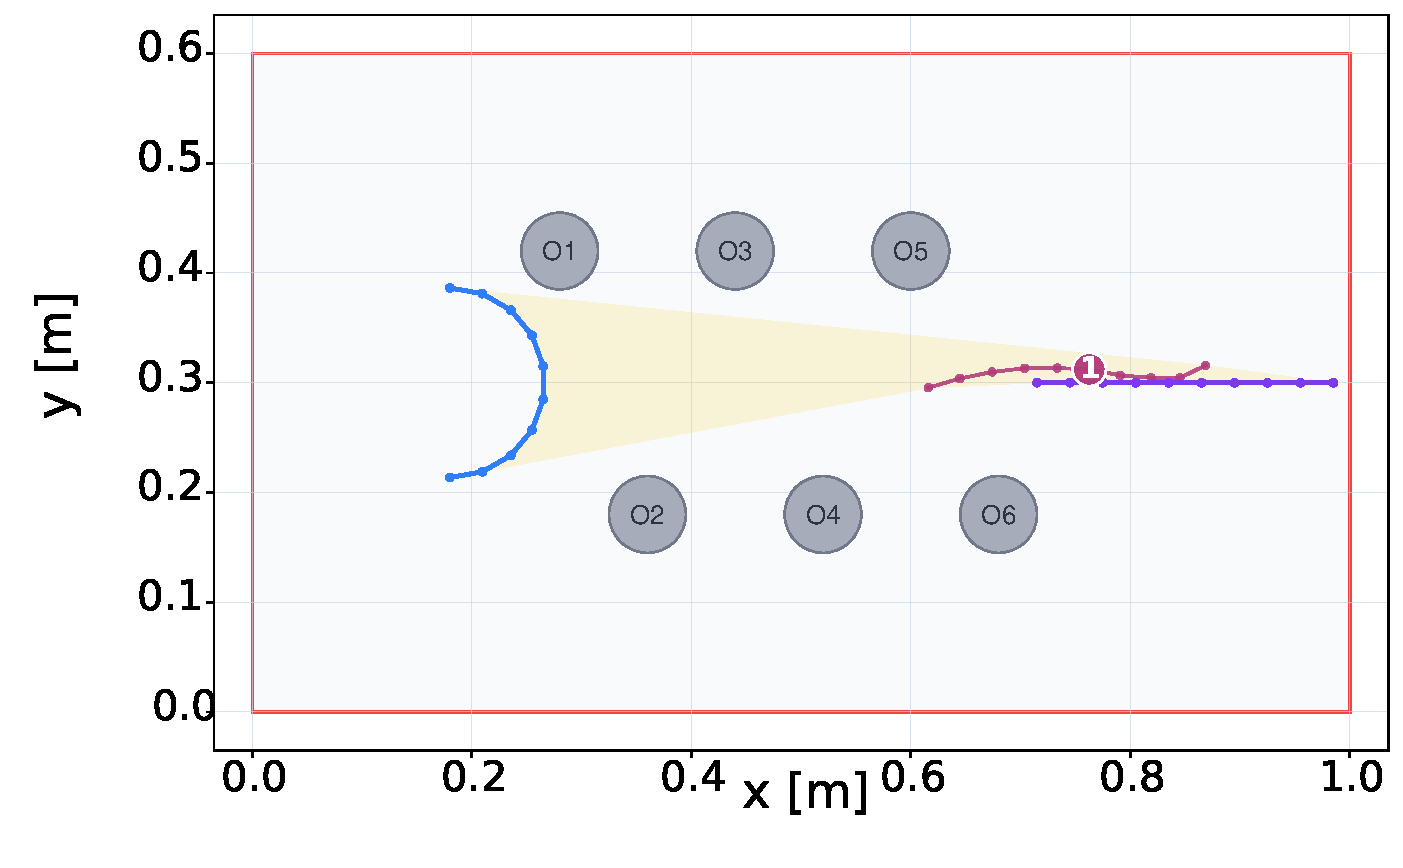
\includegraphics[width=0.3\textwidth]{figures/paper_results/scenario_05_scenario_05_arc_to_straight_fewest_config_no_legend.pdf}\label{fig:sc01}}~
    \subfloat[Scenario 2]{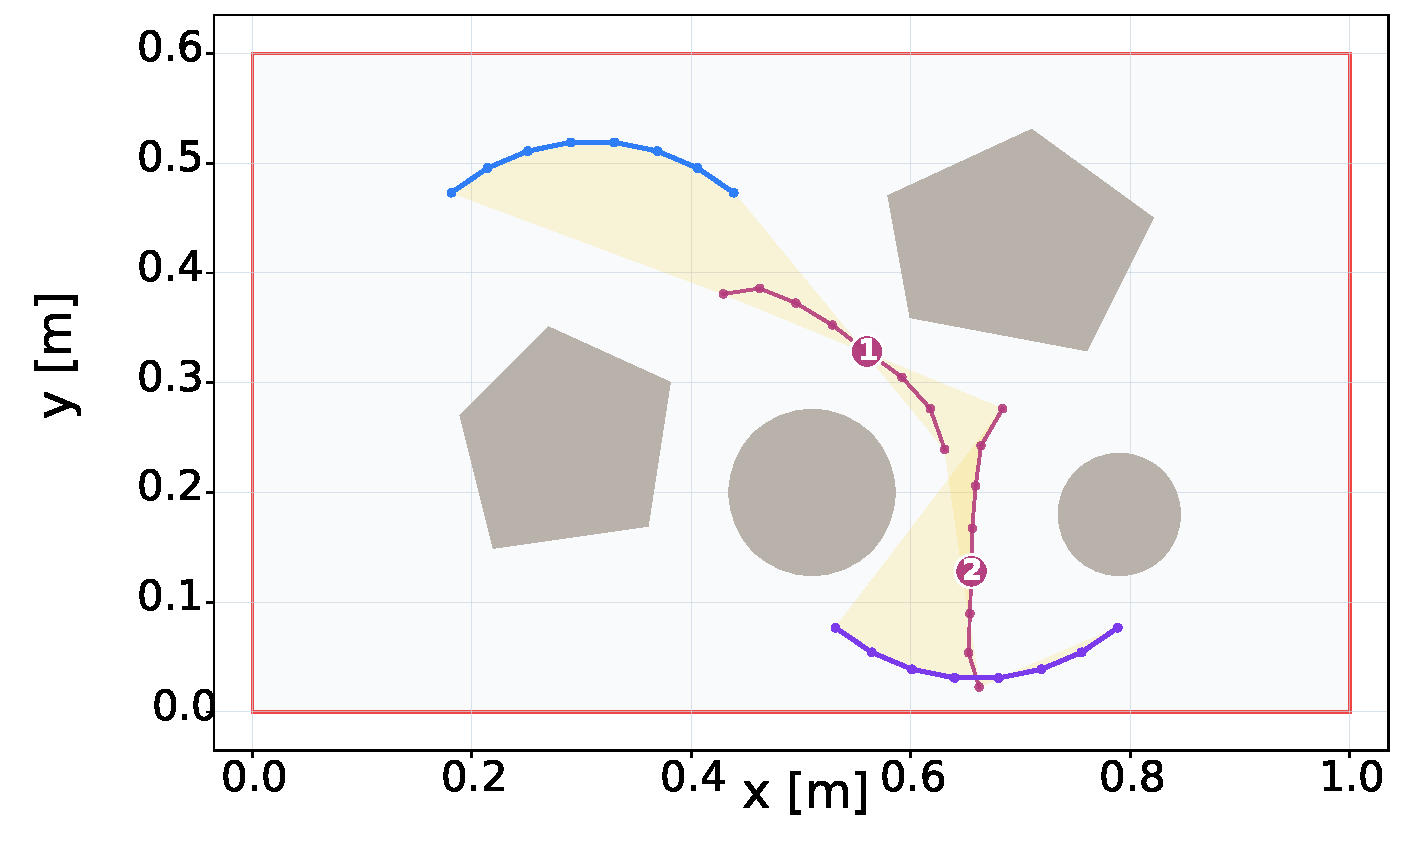
\includegraphics[width=0.3\textwidth]{figures/paper_results/scenario_08_scenario_08_dlo_workspace_fewest_config_no_legend.pdf}\label{fig:sc02}}~
    \subfloat[Scenario 3]{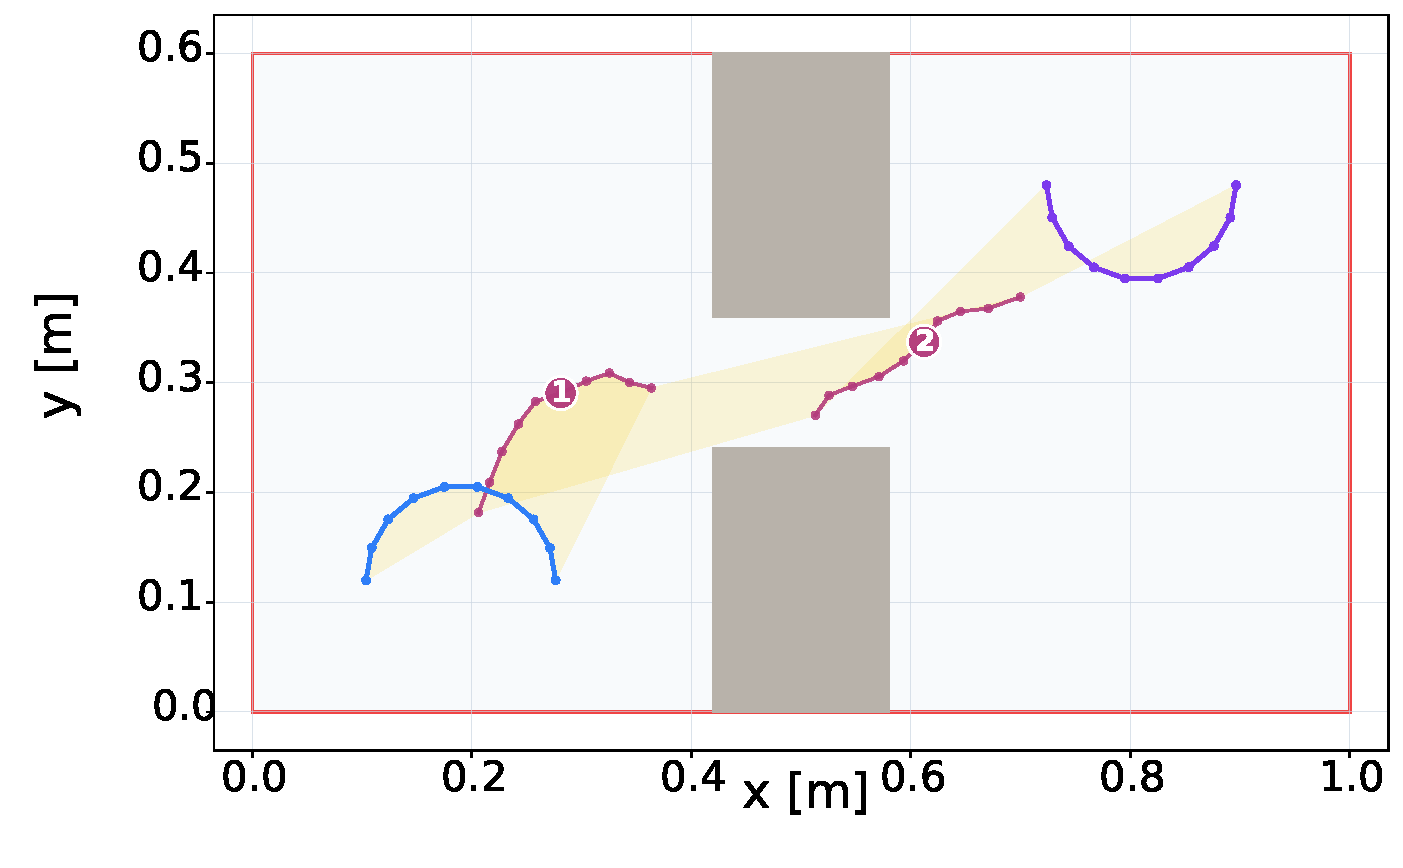
\includegraphics[width=0.3\textwidth]{figures/paper_results/scenario_11_scenario_2_narrow_gate_fewest_config_no_legend.pdf}\label{fig:sc03}}\\
    \subfloat[Scenario 4]{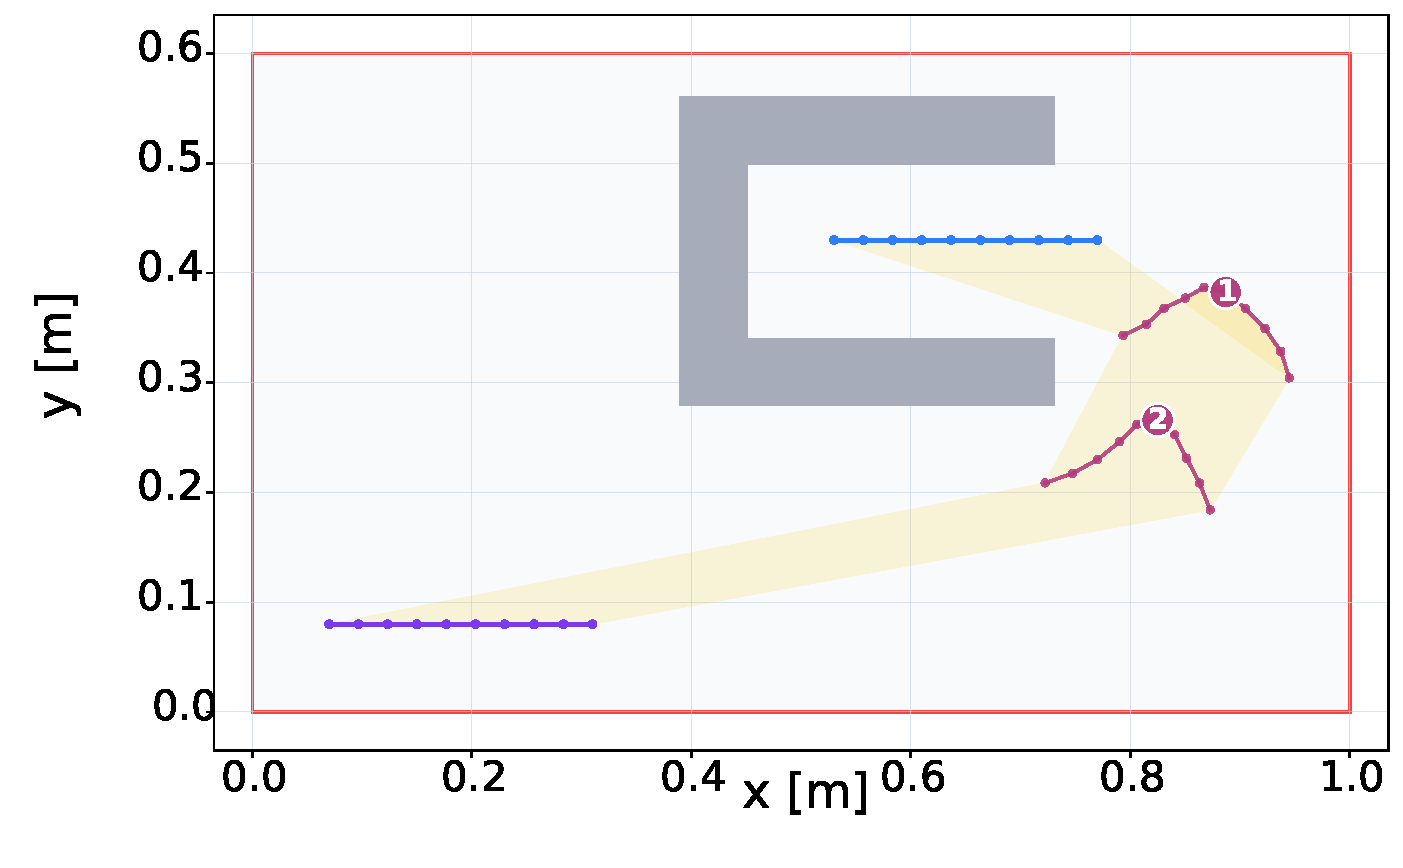
\includegraphics[width=0.3\textwidth]{figures/paper_results/scenario_12_scenario_6_u_shaped_trap_fewest_config_no_legend.pdf}\label{fig:sc04}}~
    \subfloat[Scenario 5]{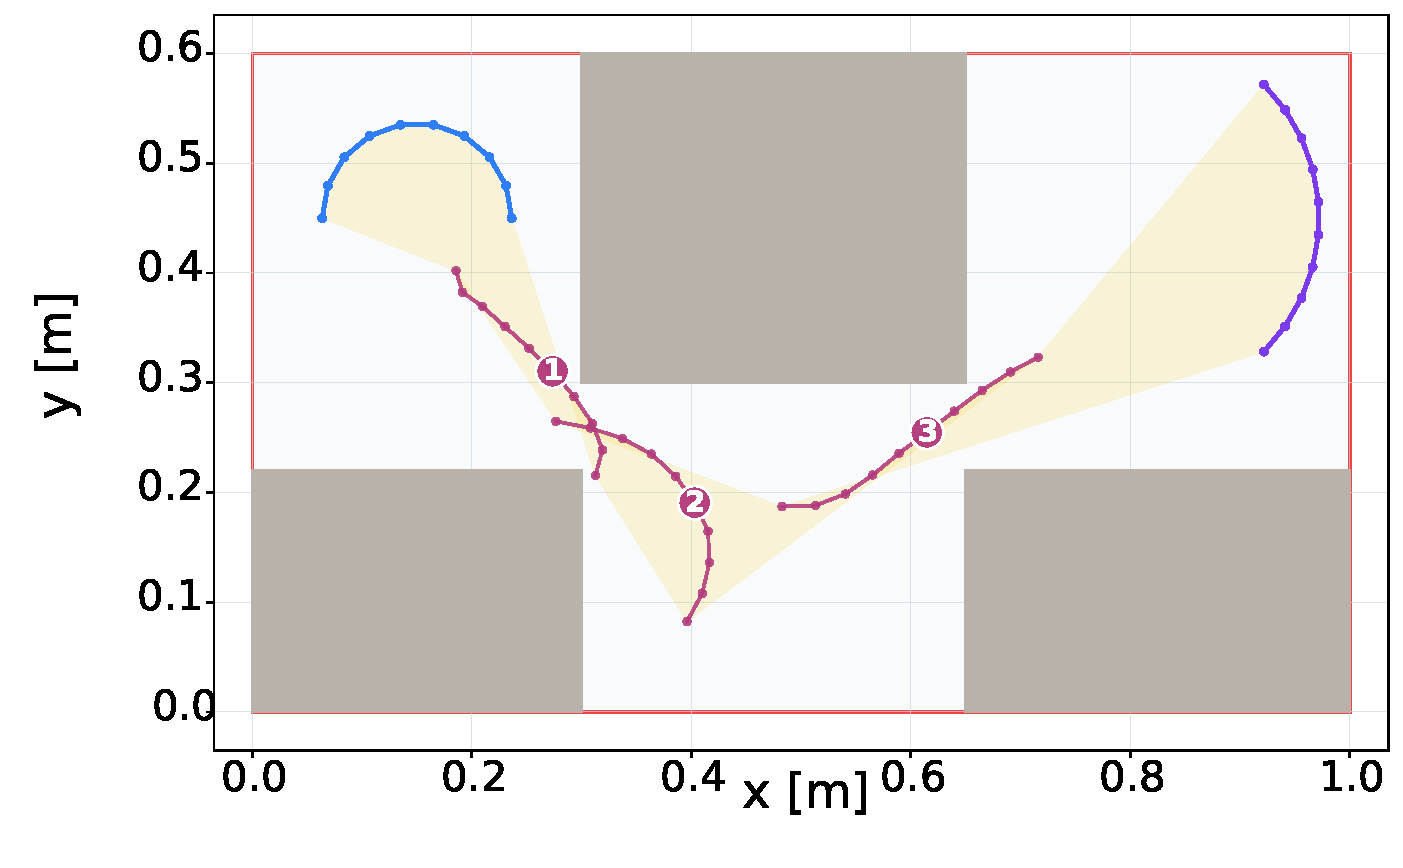
\includegraphics[width=0.3\textwidth]{figures/paper_results/scenario_09_scenario_09_S_corridor_fewest_config_no_legend.pdf}\label{fig:sc05}}~
    \subfloat[Scenario 6]{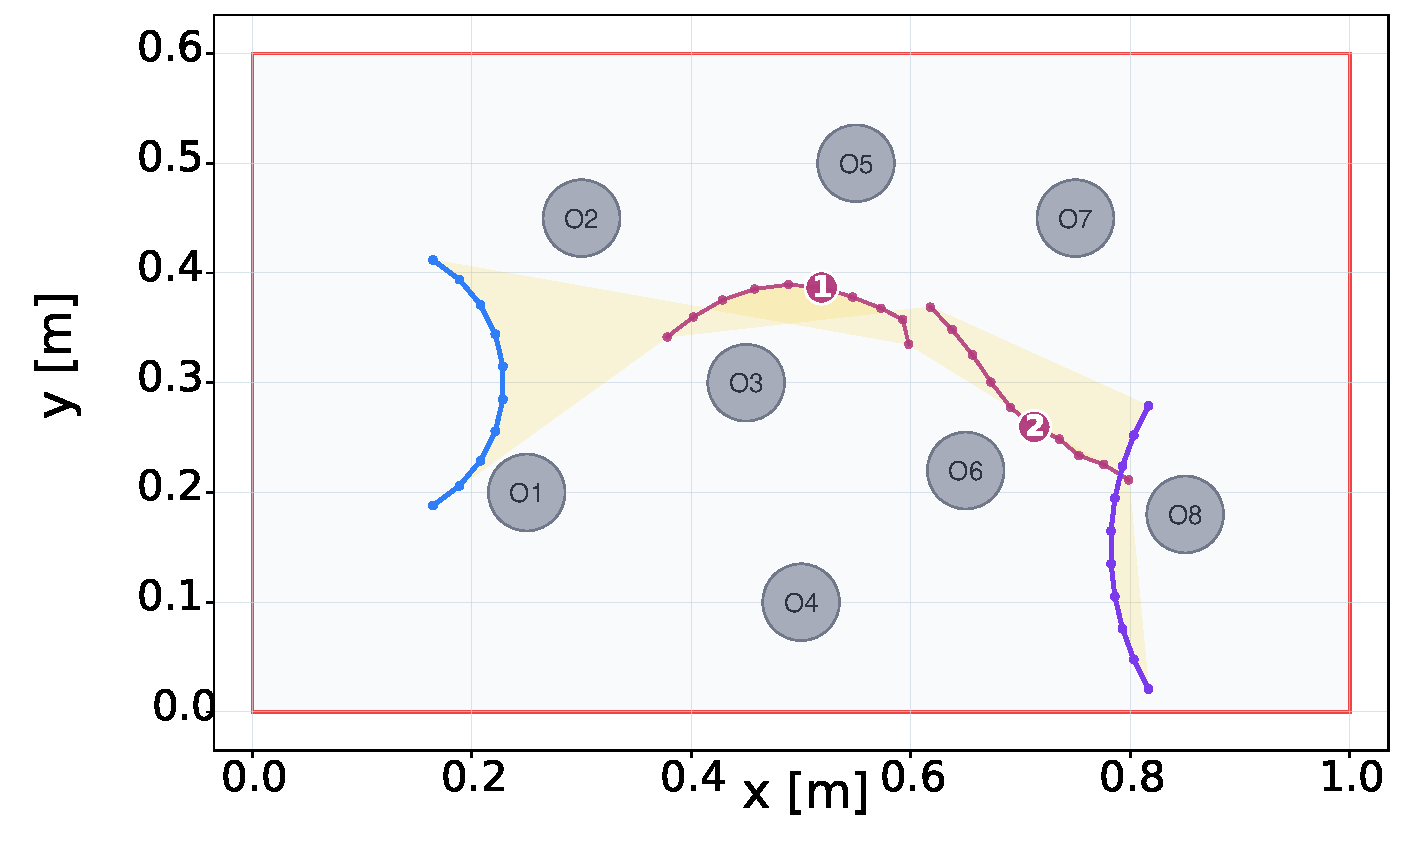
\includegraphics[width=0.3\textwidth]{figures/paper_results/scenario_10_scenario_10_cluttered_bent_fewest_config_no_legend.pdf}\label{fig:sc06}}
    \\
    \subfloat[Scenario 7]{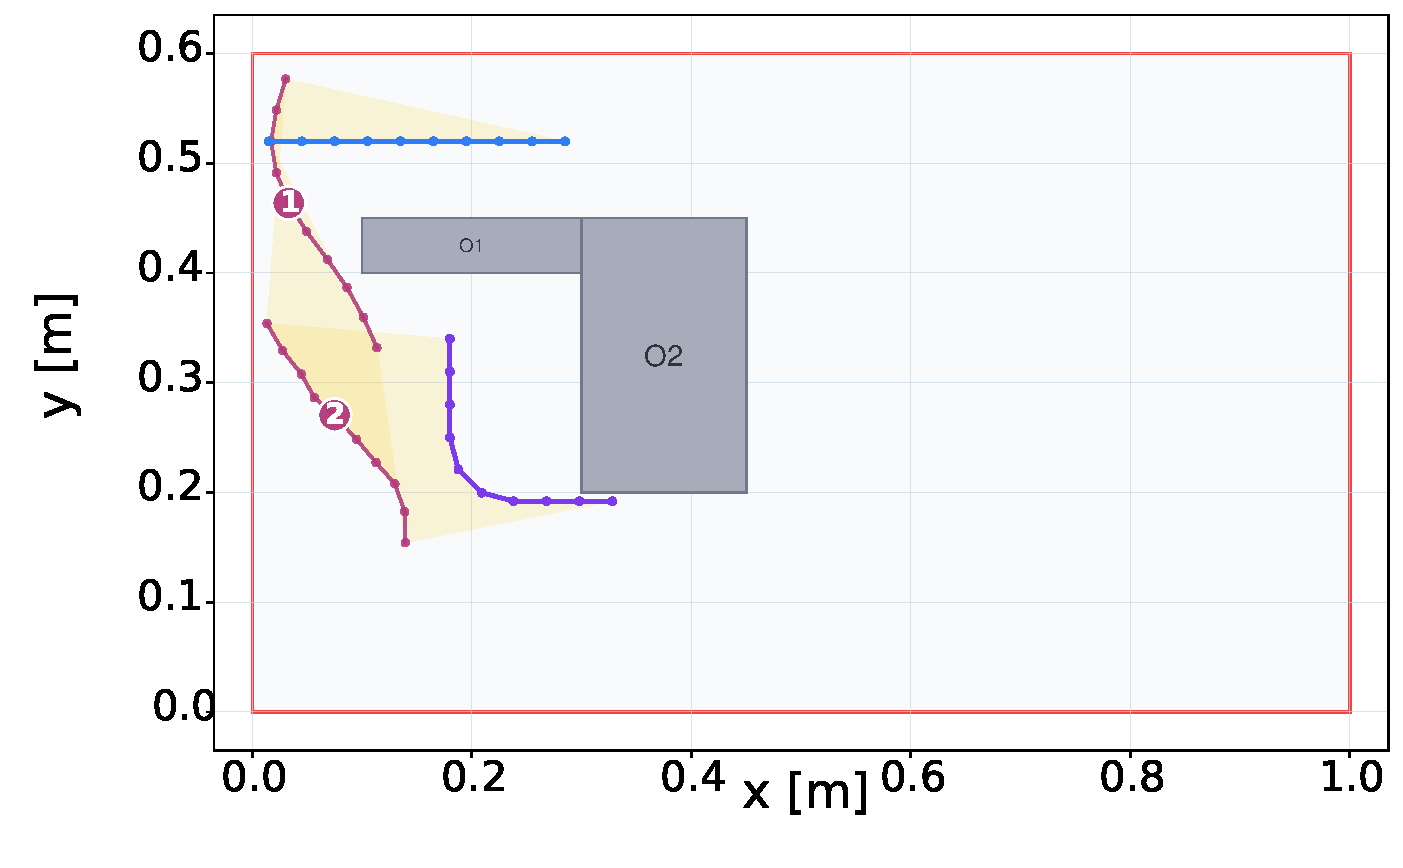
\includegraphics[width=0.3\textwidth]{figures/paper_results/scenario_02_scenario_02_block_reorient_fewest_config_no_legend.pdf}\label{fig:sc07}}~
    \subfloat[Scenario 8]{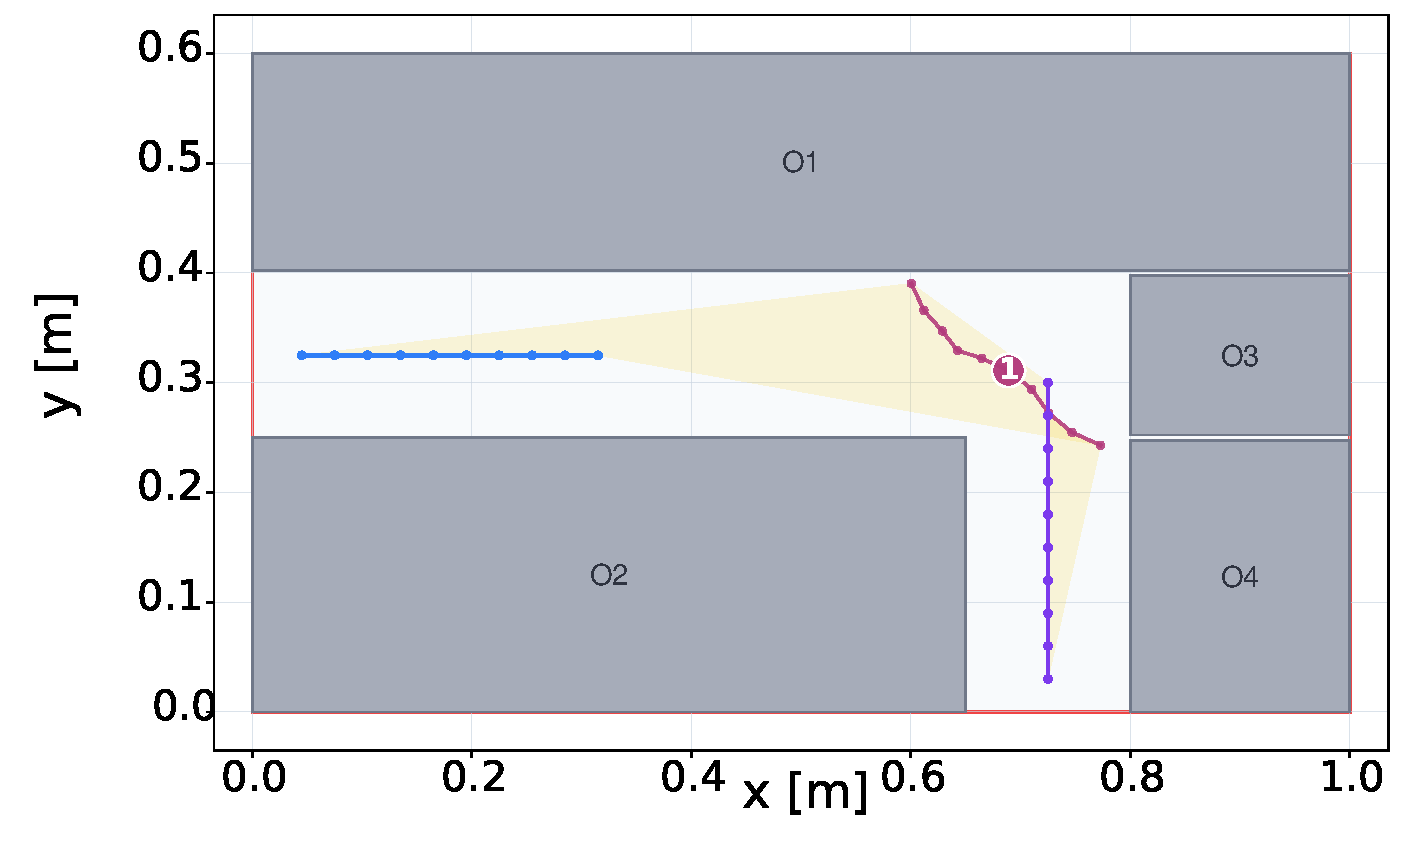
\includegraphics[width=0.3\textwidth]{figures/paper_results/scenario_03_scenario_03_L_narrow_corridor_fewest_config_no_legend.pdf}\label{fig:sc08}}~
    \subfloat[Scenario 9]{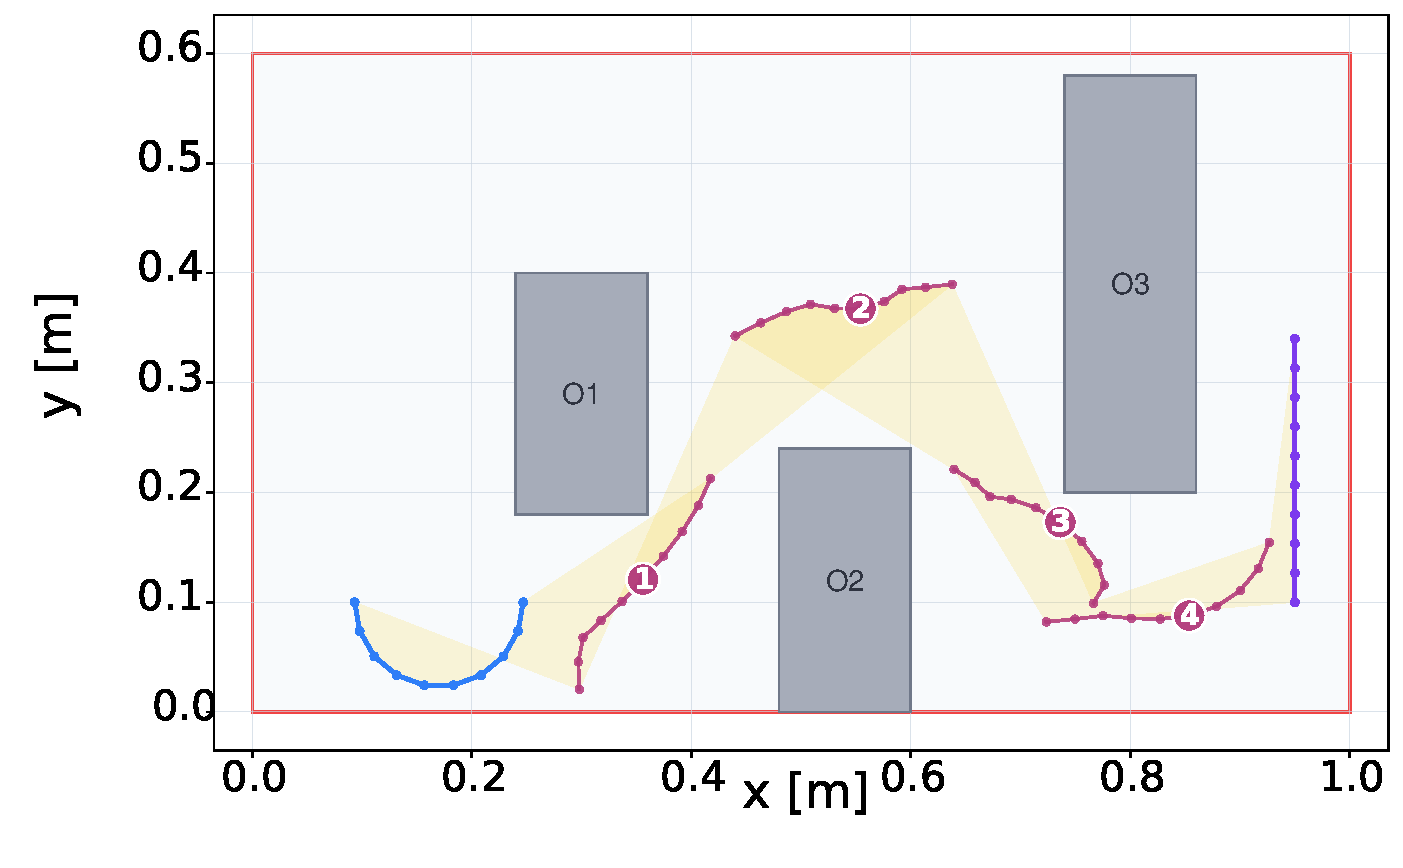
\includegraphics[width=0.3\textwidth]{figures/paper_results/scenario_14_scenario_4_staggered_blocks_fewest_config_no_legend.pdf}\label{fig:sc09}}\\
    \subfloat[Scenario 10]{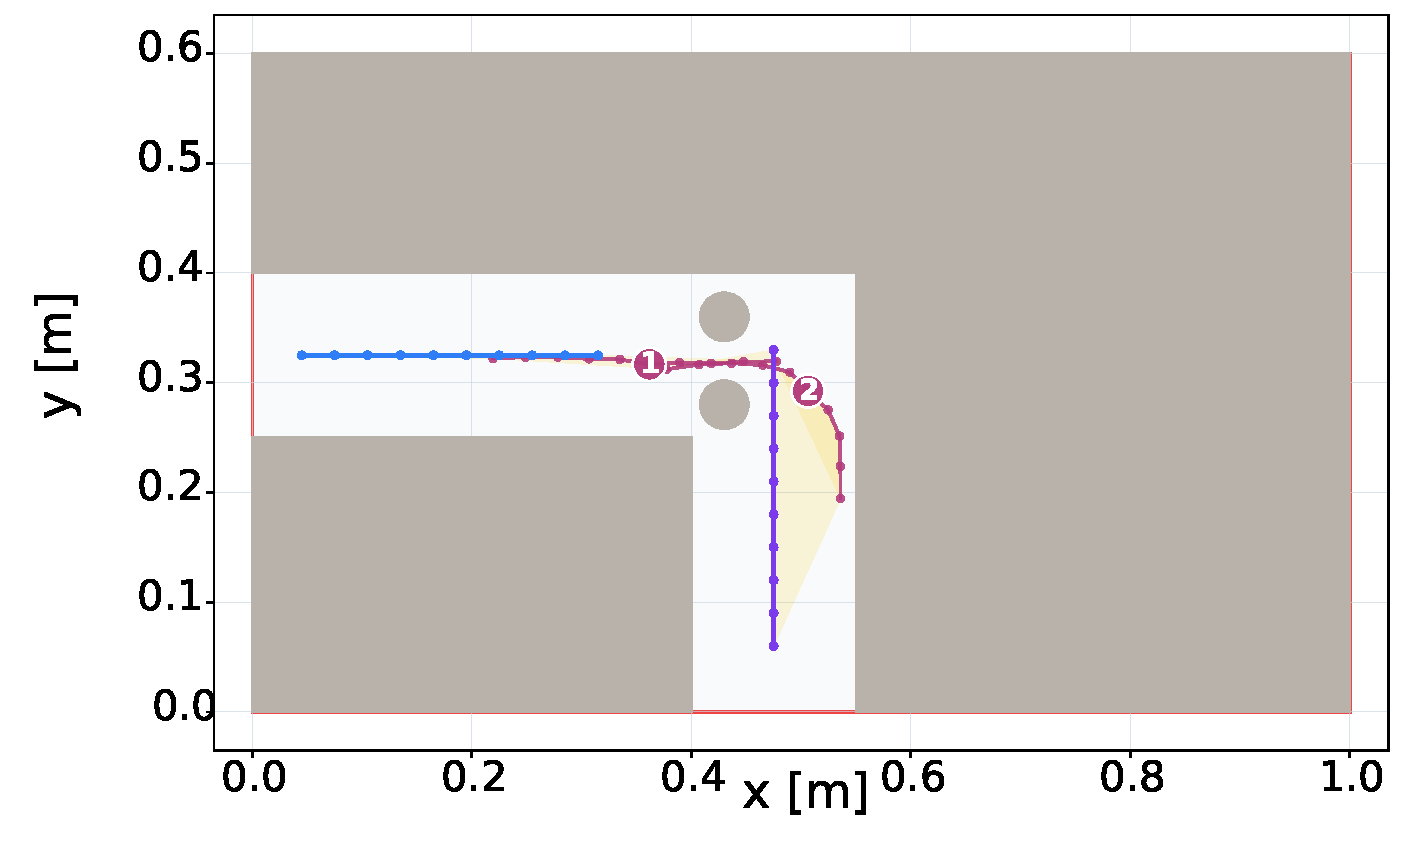
\includegraphics[width=0.3\textwidth]{figures/paper_results/scenario_07_scenario_07_L_corridor_hard_fewest_config_no_legend.pdf}\label{fig:sc10}}\\
    {
\includegraphics[width=0.8\textwidth]{figures/paper_results/paper_plot_legend.pdf}}

\caption{Representative GCR solutions for the ten benchmark scenarios. Each subfigure shows the initial cable configuration, the target cable configuration, the static obstacles, and the resulting deformation sequence.}
\label{fig:benchmark_solutions}
\end{figure*}




% \begin{figure*}[t]
% % \centering
% % \includegraphics[width=\textwidth]{figures/benchmark_solutions.png}

%  \centering
%     \subfloat[Scenario 1]{\includegraphics[width=0.4\textwidth]{figures/paper_results/scenario_05_scenario_05_arc_to_straight_fewest_config.pdf}\label{fig:sc01}}~
%     \subfloat[Scenario 2]{\includegraphics[width=0.4\textwidth]{figures/paper_results/scenario_08_scenario_08_dlo_workspace_fewest_config.pdf}\label{fig:sc02}}
%     \\
%     \subfloat[Scenario 3]{\includegraphics[width=0.4\textwidth]{figures/paper_results/scenario_11_scenario_2_narrow_gate_fewest_config.pdf}\label{fig:sc03}}~
%     \subfloat[Scenario 4]{\includegraphics[width=0.4\textwidth]{figures/paper_results/scenario_12_scenario_6_u_shaped_trap_fewest_config.pdf}\label{fig:sc04}}
%     \\
%     \subfloat[Scenario 5]{\includegraphics[width=0.4\textwidth]{figures/paper_results/scenario_09_scenario_09_S_corridor_fewest_config.pdf}\label{fig:sc05}}~
%     \subfloat[Scenario 6]{\includegraphics[width=0.4\textwidth]{figures/paper_results/scenario_10_scenario_10_cluttered_bent_fewest_config.pdf}\label{fig:sc06}}
   

% \caption{Representative GCR solutions for the ten benchmark scenarios. Each subfigure shows the initial cable configuration, the target cable configuration, the static obstacles, and the resulting deformation sequence.}
% \label{fig:benchmark_solutions1}
% \end{figure*}

% \begin{figure*}[t]
% % \centering
% % \includegraphics[width=\textwidth]{figures/benchmark_solutions.png}

%  \centering
%     \subfloat[Scenario 7]{\includegraphics[width=0.4\textwidth]{figures/paper_results/scenario_02_scenario_02_block_reorient_fewest_config.pdf}\label{fig:sc07}}~
%     \subfloat[Scenario 8]{\includegraphics[width=0.4\textwidth]{figures/paper_results/scenario_03_scenario_03_L_narrow_corridor_fewest_config.pdf}\label{fig:sc08}}
%     \\
%     \subfloat[Scenario 9]{\includegraphics[width=0.4\textwidth]{figures/paper_results/scenario_14_scenario_4_staggered_blocks_fewest_config.pdf}\label{fig:sc09}}~
%     \subfloat[Scenario 10]{\includegraphics[width=0.4\textwidth]{figures/paper_results/scenario_07_scenario_07_L_corridor_hard_fewest_config.pdf}\label{fig:sc10}}

% \caption{Representative GCR solutions for the ten benchmark scenarios. Each subfigure shows the initial cable configuration, the target cable configuration, the static obstacles, and the resulting deformation sequence.}
% \label{fig:benchmark_solutions2}
% \end{figure*}

We report the following metrics for each benchmark scenario:
\begin{itemize}
    \item \textbf{Success rate}: the percentage of trials in which GCR finds an accepted path before reaching the maximum number of iterations.
    
    \item \textbf{Average planning time}: the mean runtime of the complete planning pipeline over successful trials.
    
    \item \textbf{Fastest planning time}: the minimum runtime observed among the successful trials. This value indicates the best-case behavior of the stochastic search for a given scenario.
    
    \item \textbf{Average number of iterations}: the mean number of tree-expansion iterations required to obtain a valid connection between the two trees.
    
    \item \textbf{Configurations before refinement}: the average number of cable configurations in the raw path immediately after the two trees are connected.

    \item \textbf{Configurations after refinement}: the average number of cable configurations remaining after shortcut refinement. This metric describes the compactness of the final path that is later used for execution.
\end{itemize}

% The last two metrics are particularly relevant for manipulation.
% Each retained configuration represents an intermediate cable shape that the robots must reproduce through endpoint motion.
% A shorter sequence is easier to execute, but the refinement step cannot remove configurations if their removal violates the swept-transition feasibility condition.


\subsection{Benchmark Results}
\label{subsec:benchmark_results}




Table~\ref{tab:paper_benchmark_results} summarizes the benchmark results.

\begin{table*}[t]
    \centering
    \caption{Benchmark performance for the selected GCR scenarios.}
    \label{tab:paper_benchmark_results}
    % \scriptsize
    \setlength{\tabcolsep}{2.5pt}
    % \begin{tabularx}{\textwidth}{|c|c|c|c|c|>{\centering\arraybackslash}X|>{\centering\arraybackslash}X|}
% \hline


%  Scenario & Success (\%) & Average Time (ms) & Fastest (ms) & Iterations &  Average Configs pre rewiring & average Configs post rewiring \\
% \hline
% 1  & 100.00 & 249.2 $\pm$ 157.0 & 9.6 &2149 $\pm$ 1318 & 17 $\pm$ 4 & 5 $\pm$ 1 \\ \hline
% 2  & 100.00 & 303.0 $\pm$ 229.9 & 18.1 & 1862 $\pm$ 1399 & 20 $\pm$ 4 & 5 $\pm$ 1 \\ \hline
% 3  & 100.00 & 7.6 $\pm$ 2.9 & 1.6 &  74 $\pm$ 27 & 13 $\pm$ 2 & 3 $\pm$ 0 \\ \hline
% 4  & 100.00 & 1421.4 $\pm$ 1161.1 & 124.01 & 7375 $\pm$ 5090 & 22 $\pm$ 5 & 5 $\pm$ 1 \\ \hline
% 5  & 100.00 & 25.6 $\pm$ 153.9 & 5.0  & 98 $\pm$ 53 & 16 $\pm$ 3 & 7 $\pm$ 0 \\ \hline
% 6  & 100.00 & 147.8 $\pm$ 66.5 & 14.2 &  971 $\pm$ 446 & 18 $\pm$ 4 & 7 $\pm$ 1 \\ \hline
% 7  & 100.00 & 155.9 $\pm$ 73.7 & 20.4 & 1402 $\pm$ 627 & 19 $\pm$ 4 & 7 $\pm$ 1 \\ \hline
% 8  & 100.00 & 73.5 $\pm$ 36.8 & 7.9 & 666 $\pm$ 337 & 16 $\pm$ 3 & 6 $\pm$ 1 \\ \hline
% 9  & 100.00 & 110.5 $\pm$ 70.5 & 4.1 &  763 $\pm$ 484 & 19 $\pm$ 3 & 5 $\pm$ 1 \\ \hline
% 10 & 100.00 & 351.3 $\pm$ 163.7 & 54.4 & 2681 $\pm$ 1205 & 25 $\pm$ 4 & 9 $\pm$ 1 \\
% \hline
% \end{tabularx}
% \noindent



% \begin{tabular}{|p{0.07\textwidth}|p{0.11\textwidth}|p{0.18\textwidth}|p{0.11\textwidth}|p{0.13\textwidth}|p{0.16\textwidth}|p{0.16\textwidth}|}
% \hline
% \centering\textbf{Scenario} &
% \centering\makecell{\textbf{Success}\\\textbf{(\%)}} &
% \centering\makecell{\textbf{Time}\\\textbf{(ms)}} &
% \centering\makecell{\textbf{Fastest}\\\textbf{(ms)}} &
% \centering\textbf{Iterations} &
% \centering\makecell{\textbf{Raw Path}\\\textbf{Configurations}} &
% \centering\arraybackslash\makecell{\textbf{Refined Path}\\\textbf{Configurations}} \\
% \hline
% \centering \textbf{1} & \centering 100.00 & \centering $249.2 \pm 157.0$ & \centering 9.6 & \centering $2149 \pm 1318$ & \centering $17 \pm 4$ & \centering\arraybackslash $5 \pm 1$ \\ \hline
% \centering \textbf{2} & \centering 100.00 & \centering $303.0 \pm 229.9$ & \centering 18.1 & \centering $1862 \pm 1399$ & \centering $20 \pm 4$ & \centering\arraybackslash $5 \pm 1$ \\ \hline
% \centering \textbf{3} & \centering 100.00 & \centering $7.6 \pm 2.9$ & \centering 1.6 & \centering $74 \pm 27$ & \centering $13 \pm 2$ & \centering\arraybackslash $3 \pm 0$ \\ \hline
% \centering \textbf{4} & \centering 100.00 & \centering $1421.4 \pm 1161.1$ & \centering 124.01 & \centering $7375 \pm 5090$ & \centering $22 \pm 5$ & \centering\arraybackslash $5 \pm 1$ \\ \hline
% \centering \textbf{5} & \centering 100.00 & \centering $25.6 \pm 153.9$ & \centering 5.0 & \centering $98 \pm 53$ & \centering $16 \pm 3$ & \centering\arraybackslash $7 \pm 0$ \\ \hline
% \centering \textbf{6} & \centering 100.00 & \centering $147.8 \pm 66.5$ & \centering 14.2 & \centering $971 \pm 446$ & \centering $18 \pm 4$ & \centering\arraybackslash $7 \pm 1$ \\ \hline
% \centering \textbf{7} & \centering 100.00 & \centering $155.9 \pm 73.7$ & \centering 20.4 & \centering $1402 \pm 627$ & \centering $19 \pm 4$ & \centering\arraybackslash $7 \pm 1$ \\ \hline
% \centering \textbf{8} & \centering 100.00 & \centering $73.5 \pm 36.8$ & \centering 7.9 & \centering $666 \pm 337$ & \centering $16 \pm 3$ & \centering\arraybackslash $6 \pm 1$ \\ \hline
% \centering \textbf{9} & \centering 100.00 & \centering $110.5 \pm 70.5$ & \centering 4.1 & \centering $763 \pm 484$ & \centering $19 \pm 3$ & \centering\arraybackslash $5 \pm 1$ \\ \hline
% \centering \textbf{10} & \centering 100.00 & \centering $351.3 \pm 163.7$ & \centering 54.4 & \centering $2681 \pm 1205$ & \centering $25 \pm 4$ & \centering\arraybackslash $9 \pm 1$ \\
% \hline
% \end{tabular}


% \begin{tabular}{|p{0.07\textwidth}|p{0.11\textwidth}|p{0.18\textwidth}|p{0.11\textwidth}|p{0.13\textwidth}|p{0.16\textwidth}|p{0.16\textwidth}|}
% \hline
% \centering\textbf{Scenario} &
% \centering\makecell{\textbf{Success}\\\textbf{(\%)}} &
% \centering\makecell{\textbf{Time}\\\textbf{(s)}} &
% \centering\makecell{\textbf{Fastest}\\\textbf{(s)}} &
% \centering\textbf{Iterations} &
% \centering\makecell{\textbf{Raw Path}\\\textbf{Configurations}} &
% \centering\arraybackslash\makecell{\textbf{Refined Path}\\\textbf{Configurations}} \\
% \hline
% \centering \textbf{1} & \centering 100.00 & \centering $0.240 \pm 0.143$ & \centering 0.010 & \centering $2076 \pm 1205$ & \centering $17 \pm 4$ & \centering\arraybackslash $5 \pm 1$ \\ \hline
% \centering \textbf{2} & \centering 100.00 & \centering $0.283 \pm 0.197$ & \centering 0.018 & \centering $1745 \pm 1213$ & \centering $20 \pm 4$ & \centering\arraybackslash $5 \pm 1$ \\ \hline
% \centering \textbf{3} & \centering 100.00 & \centering $0.008 \pm 0.003$ & \centering 0.002 & \centering $73 \pm 26$ & \centering $13 \pm 2$ & \centering\arraybackslash $3 \pm 0$ \\ \hline
% \centering \textbf{4} & \centering 100.00 & \centering $1.306 \pm 0.871$ & \centering 0.124 & \centering $6980 \pm 4524$ & \centering $22 \pm 5$ & \centering\arraybackslash $5 \pm 1$ \\ \hline
% \centering \textbf{5} & \centering 100.00 & \centering $0.017 \pm 0.005$ & \centering 0.005 & \centering $95 \pm 31$ & \centering $16 \pm 3$ & \centering\arraybackslash $7 \pm 0$ \\ \hline
% \centering \textbf{6} & \centering 100.00 & \centering $0.145 \pm 0.061$ & \centering 0.014 & \centering $951 \pm 418$ & \centering $18 \pm 4$ & \centering\arraybackslash $7 \pm 1$ \\ \hline
% \centering \textbf{7} & \centering 100.00 & \centering $0.151 \pm 0.066$ & \centering 0.020 & \centering $1359 \pm 566$ & \centering $19 \pm 4$ & \centering\arraybackslash $7 \pm 1$ \\ \hline
% \centering \textbf{8} & \centering 100.00 & \centering $0.072 \pm 0.033$ & \centering 0.008 & \centering $648 \pm 309$ & \centering $16 \pm 3$ & \centering\arraybackslash $6 \pm 1$ \\ \hline
% \centering \textbf{9} & \centering 100.00 & \centering $0.104 \pm 0.059$ & \centering 0.004 & \centering $719 \pm 412$ & \centering $18 \pm 3$ & \centering\arraybackslash $5 \pm 1$ \\ \hline
% \centering \textbf{10} & \centering 100.00 & \centering $0.339 \pm 0.139$ & \centering 0.054 & \centering $2597 \pm 1077$ & \centering $25 \pm 4$ & \centering\arraybackslash $9 \pm 1$ \\
% \hline
% \end{tabular}


\begin{tabular}{|p{0.07\textwidth}|p{0.11\textwidth}|p{0.18\textwidth}|p{0.11\textwidth}|p{0.13\textwidth}|p{0.16\textwidth}|p{0.16\textwidth}|}
\hline
\centering\textbf{Scenario} &
\centering\makecell{\textbf{Success}\\\textbf{(\%)}} &
\centering\makecell{\textbf{Time}\\\textbf{(s)}} &
\centering\makecell{\textbf{Fastest}\\\textbf{(s)}} &
\centering\makecell{\textbf{Iterations}\\\textbf{($10^3$)}}  &
\centering\makecell{\textbf{Raw Path}\\\textbf{Configurations}} &
\centering\arraybackslash\makecell{\textbf{Refined Path}\\\textbf{Configurations}} \\
\hline
\centering \textbf{1} & \centering 100.00 & \centering $0.240 \pm 0.143$ & \centering 0.010 & \centering $2.08 \pm 1.20$ & \centering $17 \pm 4$ & \centering\arraybackslash $5 \pm 1$ \\ \hline
\centering \textbf{2} & \centering 100.00 & \centering $0.283 \pm 0.197$ & \centering 0.018 & \centering $1.75 \pm 1.21$ & \centering $20 \pm 4$ & \centering\arraybackslash $5 \pm 1$ \\ \hline
\centering \textbf{3} & \centering 100.00 & \centering $0.008 \pm 0.003$ & \centering 0.002 & \centering $0.07 \pm 0.03$ & \centering $13 \pm 2$ & \centering\arraybackslash $3 \pm 0$ \\ \hline
\centering \textbf{4} & \centering 100.00 & \centering $1.306 \pm 0.871$ & \centering 0.124 & \centering $6.98 \pm 4.52$ & \centering $22 \pm 5$ & \centering\arraybackslash $5 \pm 1$ \\ \hline
\centering \textbf{5} & \centering 100.00 & \centering $0.017 \pm 0.005$ & \centering 0.005 & \centering $0.09 \pm 0.03$ & \centering $16 \pm 3$ & \centering\arraybackslash $7 \pm 0$ \\ \hline
\centering \textbf{6} & \centering 100.00 & \centering $0.145 \pm 0.061$ & \centering 0.014 & \centering $0.95 \pm 0.42$ & \centering $18 \pm 4$ & \centering\arraybackslash $7 \pm 1$ \\ \hline
\centering \textbf{7} & \centering 100.00 & \centering $0.151 \pm 0.066$ & \centering 0.020 & \centering $1.36 \pm 0.57$ & \centering $19 \pm 4$ & \centering\arraybackslash $7 \pm 1$ \\ \hline
\centering \textbf{8} & \centering 100.00 & \centering $0.072 \pm 0.033$ & \centering 0.008 & \centering $0.65 \pm 0.31$ & \centering $16 \pm 3$ & \centering\arraybackslash $6 \pm 1$ \\ \hline
\centering \textbf{9} & \centering 100.00 & \centering $0.104 \pm 0.059$ & \centering 0.004 & \centering $0.72 \pm 0.41$ & \centering $18 \pm 3$ & \centering\arraybackslash $5 \pm 1$ \\ \hline
\centering \textbf{10} & \centering 100.00 & \centering $0.339 \pm 0.139$ & \centering 0.054 & \centering $2.60 \pm 1.08$ & \centering $25 \pm 4$ & \centering\arraybackslash $9 \pm 1$ \\
\hline
\end{tabular}

\end{table*}

GCR found a valid path in every trial, giving a 100\% success rate in all ten scenarios.
This result should be interpreted within the tested scenario set; it shows that the implemented combination of bidirectional expansion, APF-biased sampling, elastic relaxation, and ordered swept-transition validation was sufficient for these planar layouts.

The computational cost varies with the geometric constraints of the workspace.
\textbf{Scenario~3}, Figure~\ref{fig:sc03}, is solved with the lowest average computation time, $0.008 \pm 0.003$~s, and requires only $(0.07 \pm 0.03)\times 10^3$ iterations on average.
This scenario represents a relatively simple routing case, where the free space allows a direct deformation sequence between $C_{\mathrm{start}}$ and $C_{\mathrm{goal}}$.
\textbf{Scenario~5}, Figure~\ref{fig:sc05}, also remains computationally light, with an average time of $0.017 \pm 0.005$~s and $(0.09 \pm 0.03)\times 10^3$ iterations.
Most trials are solved quickly, as indicated by the fastest time of 0.005~s.

The most demanding case is \textbf{Scenario~4}, Figure~\ref{fig:sc04}, where the planner requires $1.306 \pm 0.871$~s and $(6.98 \pm 4.52)\times 10^3$ iterations on average.
This increase is consistent with the more constrained obstacle arrangement, where the cable has fewer admissible deformation routes and the planner must reject more samples because of static collisions or invalid swept transitions.
\textbf{Scenario~10}, Figure~\ref{fig:sc10}, is the second most expensive case, with $0.339 \pm 0.139$~s and $(2.60 \pm 1.08)\times 10^3$ iterations.

For the remaining scenarios, \textbf{Scenarios~1, 2, 6, 7, 8, and~9} shown in Figure~\ref{fig:benchmark_solutions}, the average runtime ranges from 0.072~s to 0.283~s.
These values show that the planner handled the selected static-obstacle tasks efficiently, except when the geometry imposed narrow or highly constrained deformation routes.

The shortcut refinement step also affects the final path representation.
Before refinement, the raw connected paths contain between $13 \pm 2$ and $25 \pm 4$ configurations on average.
After refinement, the final paths contain between $3$ and $9 \pm 1$ configurations.
The retained configurations are those that preserve the validity of the cable transition according to the swept-envelope test and ordered edge-feasibility validation.

Overall, the average computation time stays below 0.34~s in nine out of ten scenarios, and the most constrained scenario is solved in about 1.31~s on average.
Runtimes of this order leave a comfortable margin for computing cable-routing sequences before execution.

\subsection{Robotic Manipulation Validation}
\label{subsec:manipulation_validation}

The second validation stage evaluates whether the refined GCR paths can guide a simulated dual-arm robotic system to deform and translate a cable.
The robotic setup, built in MuJoCo~\citep{todorov2012mujoco}, is shown in Fig.~\ref{fig:mujoco_setup}.
It contains two UR10 manipulators attached rigidly to the two cable ends, the target cable shape, and the bounded planar workspace with obstacles. The robots track the planned endpoint trajectories, while the internal cable elements move passively according to the simulated cable dynamics, elasticity, gravity, contact response, and endpoint motion.

\begin{figure}
    \centering
    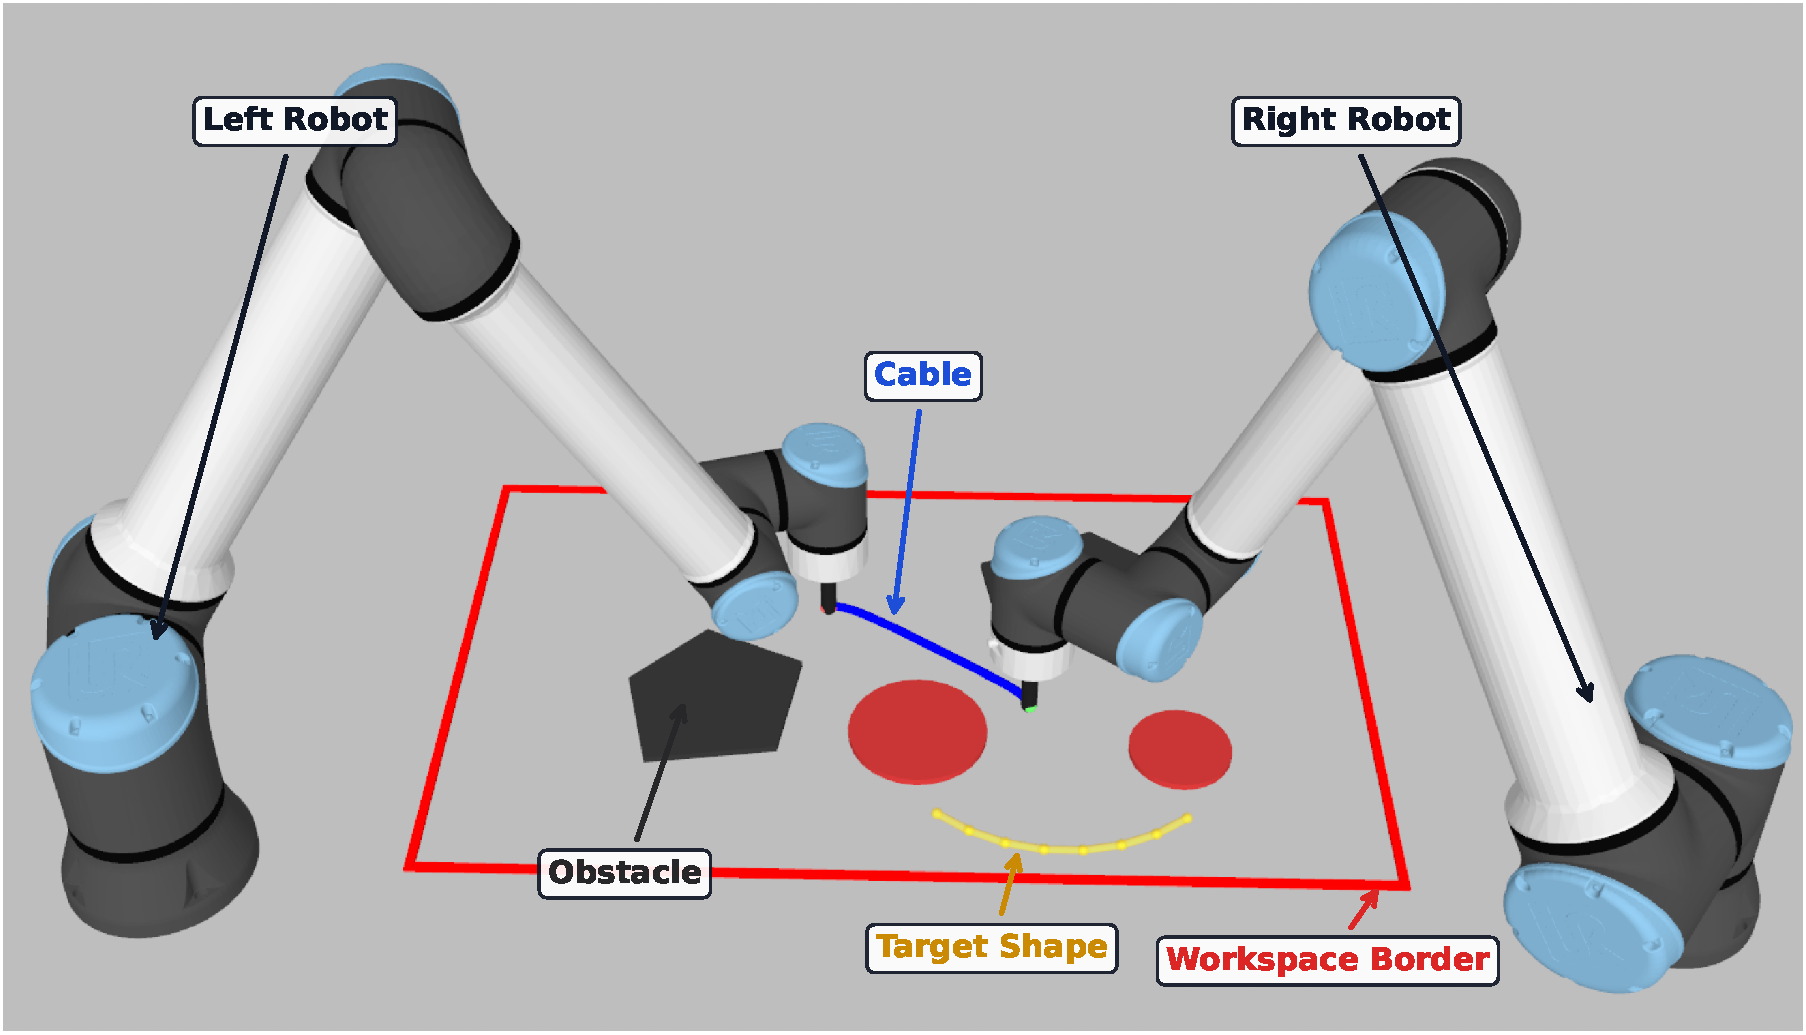
\includegraphics[width=0.95\linewidth]{figures/simulation_setup_annotated.pdf}
    \caption{Dual-arm MuJoCo setup used for simulation-based manipulation validation.}
    \label{fig:mujoco_setup}
\end{figure}

For each waypoint configuration, the first and last cable points define the Cartesian references for the left and right robot end-effectors.
The endpoint motion between two consecutive configurations is executed using smooth task-space interpolation.
The settled cable configuration at the end of the execution is then compared with the planned goal configuration.

\subsection{Robotic Execution Results}
\label{subsec:robotic_results}

Table~\ref{tab:robotic_validation} reports the execution accuracy for the scenarios. The root mean square error (\(\mathrm{RMSE}\)) and maximum point-wise error (\(e_{\max}\)) are computed over all cable nodes between the settled simulation state and the goal configuration.

\begin{equation}
    e_{\max} = \max(e_1, e_2, \dots, e_N)
\end{equation}

\begin{equation}
    \mathrm{RMSE} = \sqrt{\frac{1}{N}\sum_{n=1}^{N} e_n^2}
\end{equation}
where $e_n$ is the Euclidean error between the $n$-th point of the final settled configuration and the corresponding point of the target configuration.

% \begin{table*}[t]
% \centering
% \caption{MuJoCo execution validation results for six selected scenarios. The final cable configuration is compared against the planned goal after a 10-second settling period.}
% \label{tab:mujoco_results}
% \begin{tabular}{ccccc}
% \hline
% Scenario & Nodes & RMS Error (mm) & Max Error (mm) & Left / Right Endpoint Error (mm) \
% \hline
% 1  & 37 & 4.66 & 7.81 & 1.60 / 2.54 \
% 3  & 37 & 2.20 & 3.41 & 0.88 / 1.10 \
% 4  & 37 & 2.83 & 4.73 & 0.97 / 0.66 \
% 5  & 29 & 2.22 & 3.72 & 0.97 / 0.96 \
% 6  & 37 & 1.51 & 2.84 & 1.17 / 0.96 \
% 10 & 37 & 4.58 & 7.32 & 1.00 / 0.90 \
% \hline
% \end{tabular}
% \end{table*}


\begin{table}[t]
    \centering
    \caption{Robotic manipulation validation results.}
    \label{tab:robotic_validation}
    % \scriptsize
    % \setlength{\tabcolsep}{2.5pt}
    \noindent
    \begin{tabular}{|c|c|c|}
        \hline
        \hfil \textbf{Scenario}\hfil & \hfil \textbf{RMSE (mm)}\hfil & \hfil \textbf{\(e_{\max}\) (mm)}\hfil \\
        \hline
         \textbf{1}  &  2.20 &  3.41 \\ \hline
         \textbf{2}  &  2.22 &  3.72 \\ \hline
         \textbf{3}  &  4.32 &  6.49 \\ \hline
         \textbf{4}  &  1.60 &  2.31 \\ \hline
         \textbf{5}  &  1.87 &  2.70 \\ \hline
         \textbf{6}  &  2.08 &  3.32 \\ \hline
         \textbf{7}  &  4.66 &  7.81 \\ \hline
         \textbf{8}  &  4.13 &  6.28 \\ \hline
         \textbf{9}  &  4.58 &  7.32 \\ \hline
         \textbf{10} &  2.83 &  4.73 \\ \hline
    \end{tabular}
\end{table}




% Figures from simulation




\begin{figure*}[t]
    \centering
    % \scriptsize
    \setlength{\tabcolsep}{2pt}
    \begin{tabular}{ccccc}
        \textbf{Scenario} & \textbf{Start} & \textbf{33\%} & \textbf{67\%} & \textbf{End} \\ \hline
        \textbf{1} &
        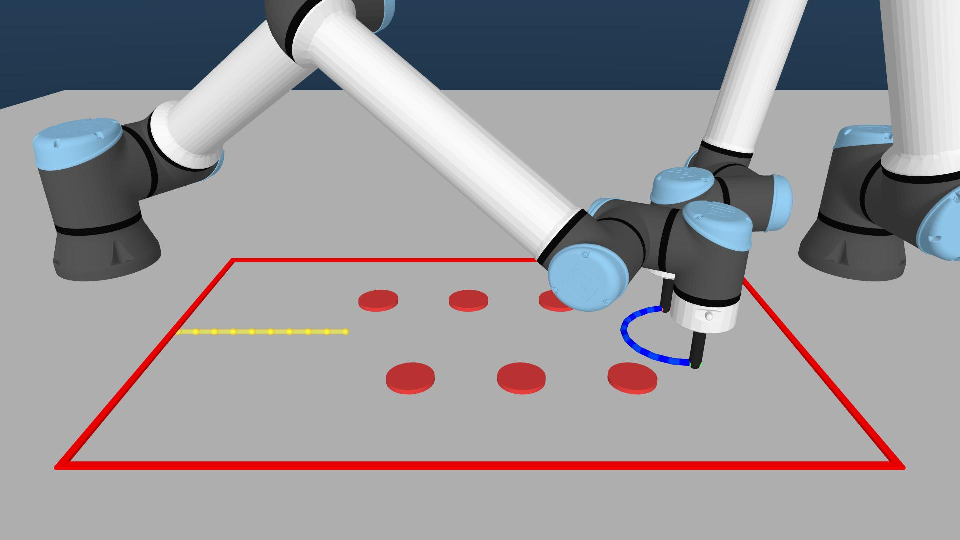
\includegraphics[width=0.21\textwidth]{figures/mujoco/scenario_01/start.pdf} &
        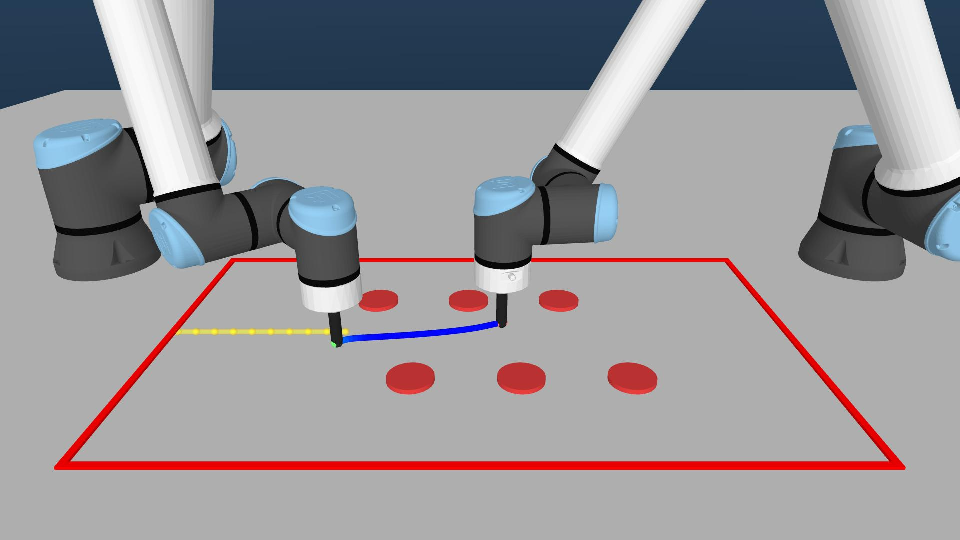
\includegraphics[width=0.21\textwidth]{figures/mujoco/scenario_01/33pct.pdf} &
        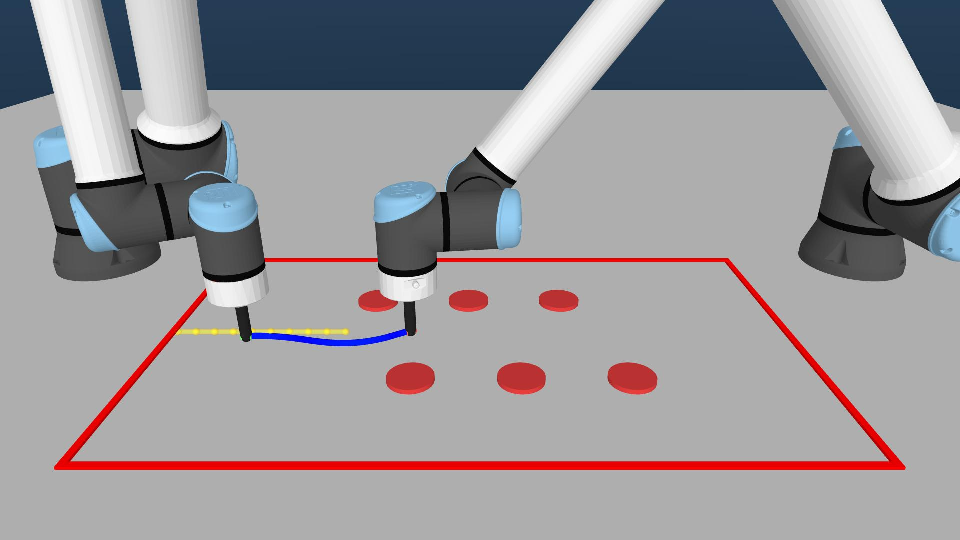
\includegraphics[width=0.21\textwidth]{figures/mujoco/scenario_01/67pct.pdf} &
        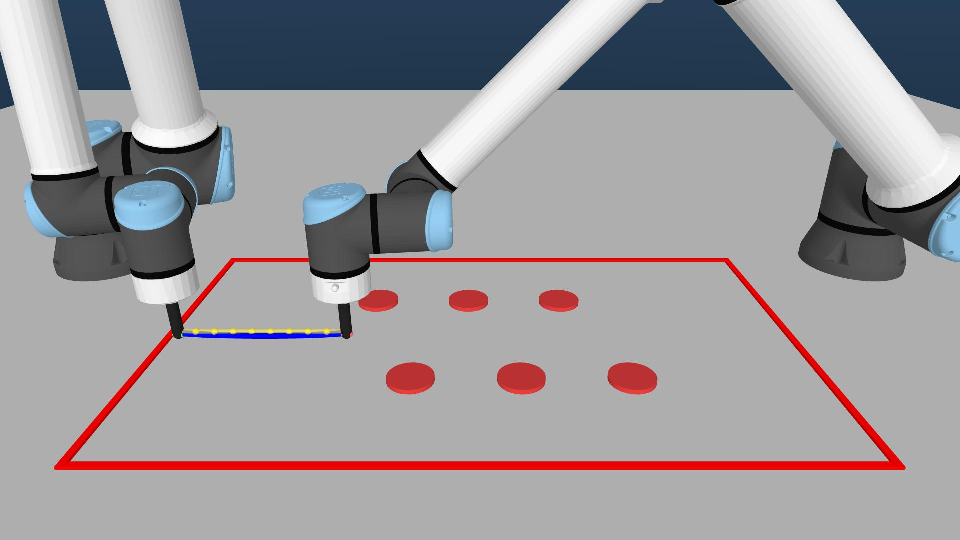
\includegraphics[width=0.21\textwidth]{figures/mujoco/scenario_01/end.pdf} \\ \hline
        \textbf{2} &
        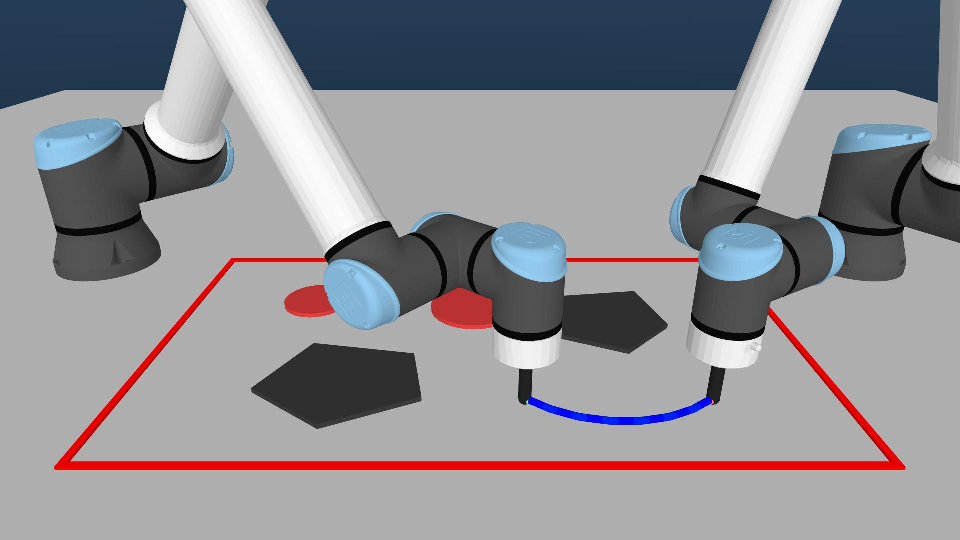
\includegraphics[width=0.21\textwidth]{figures/mujoco/scenario_02/start.pdf} &
        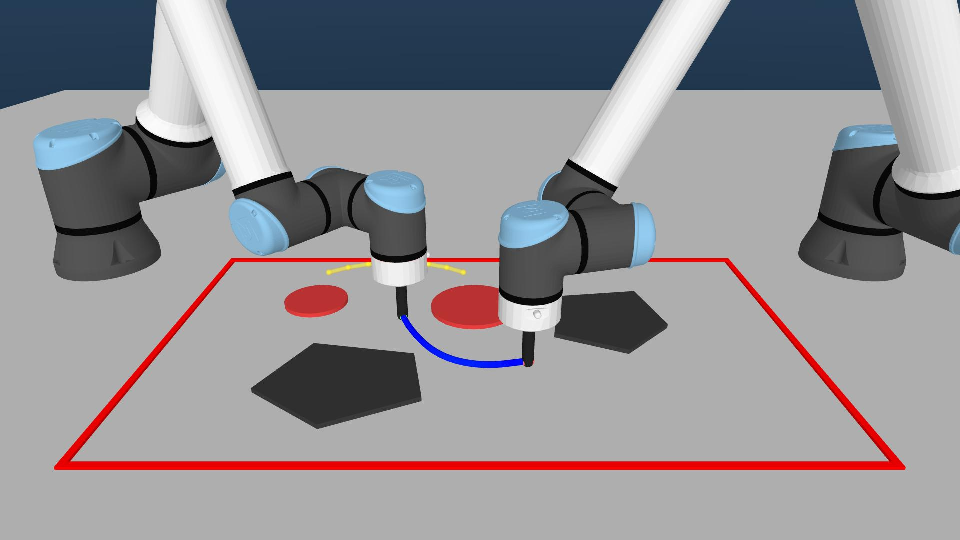
\includegraphics[width=0.21\textwidth]{figures/mujoco/scenario_02/33pct.pdf} &
        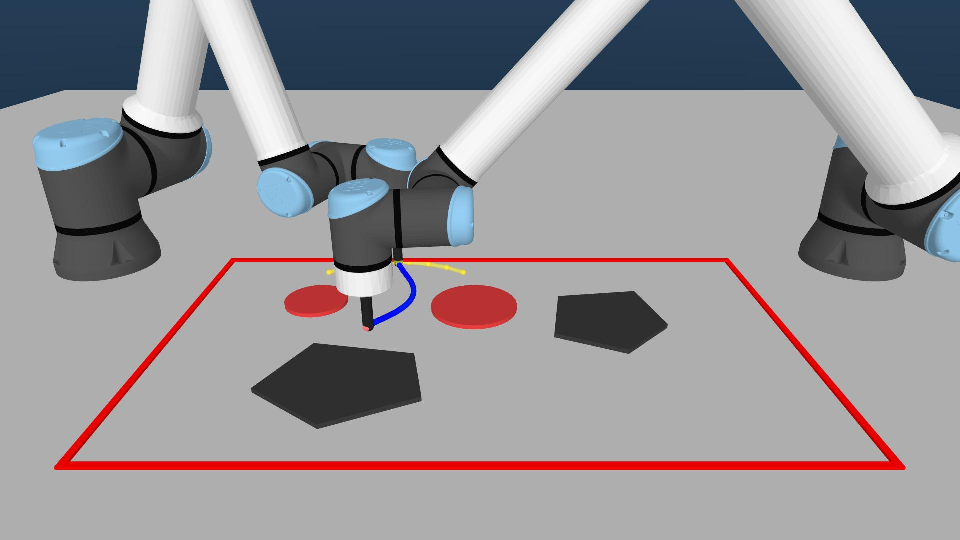
\includegraphics[width=0.21\textwidth]{figures/mujoco/scenario_02/67pct.pdf} &
        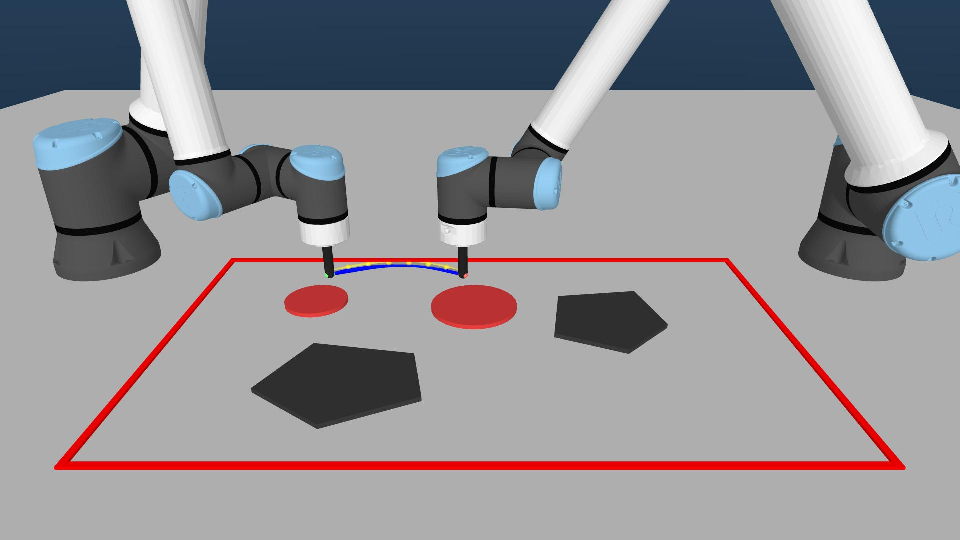
\includegraphics[width=0.21\textwidth]{figures/mujoco/scenario_02/end.pdf} \\ \hline
        \textbf{5} &
        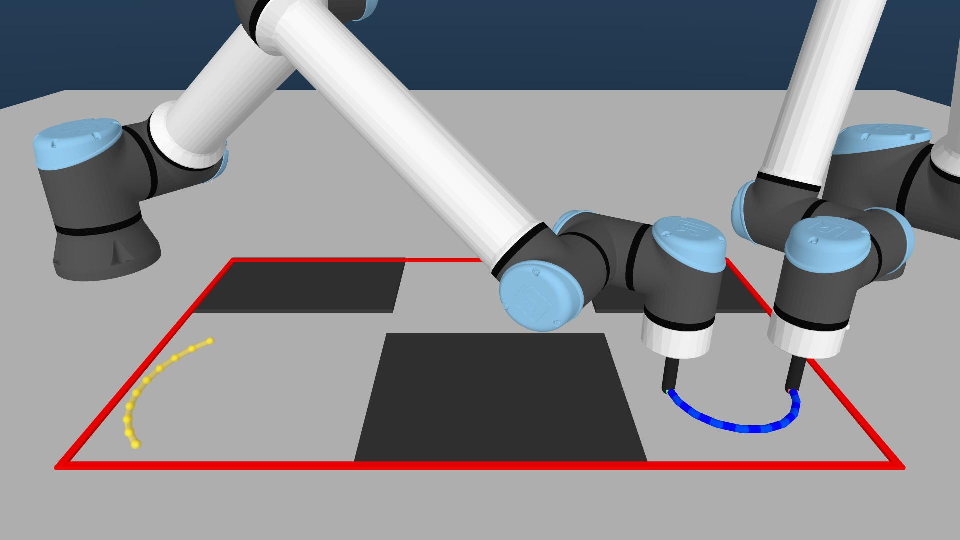
\includegraphics[width=0.21\textwidth]{figures/mujoco/scenario_05/start.pdf} &
        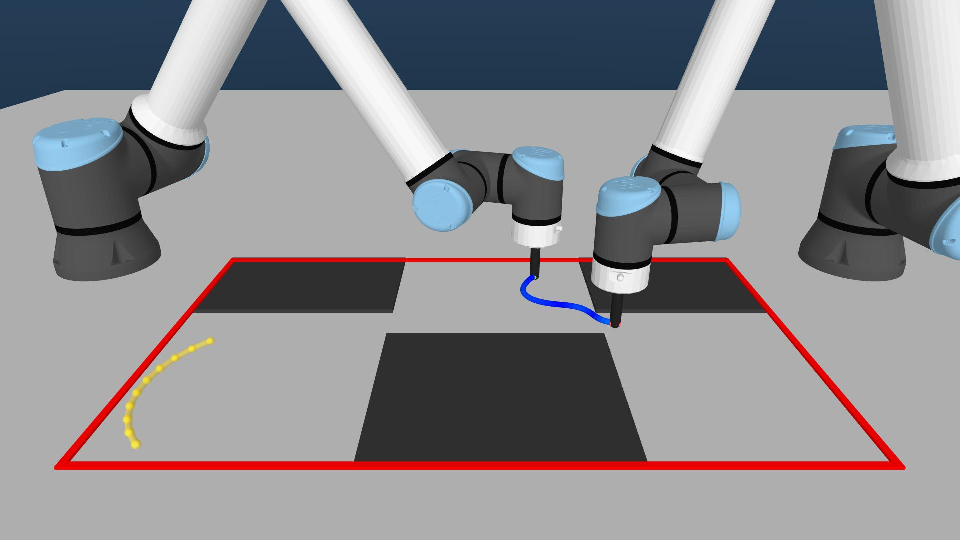
\includegraphics[width=0.21\textwidth]{figures/mujoco/scenario_05/33pct.pdf} &
        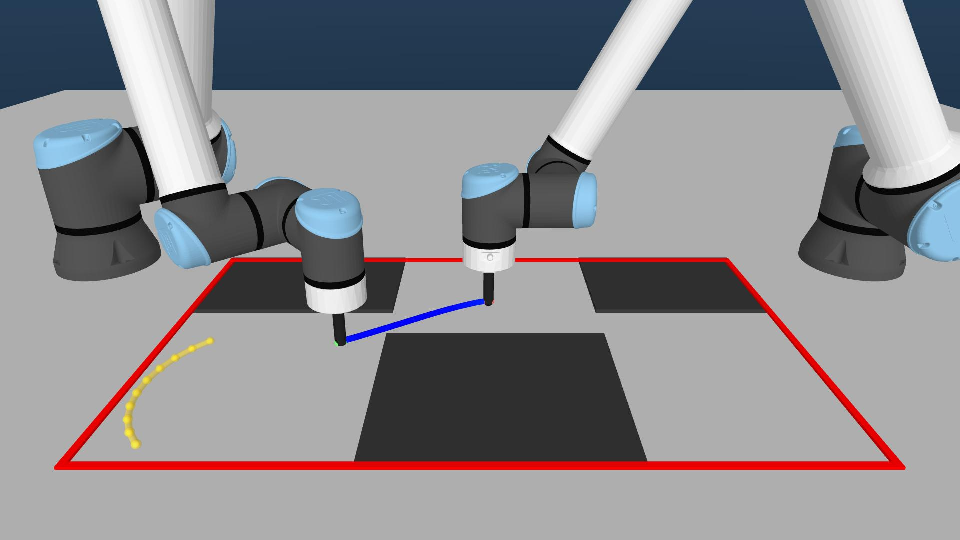
\includegraphics[width=0.21\textwidth]{figures/mujoco/scenario_05/67pct.pdf} &
        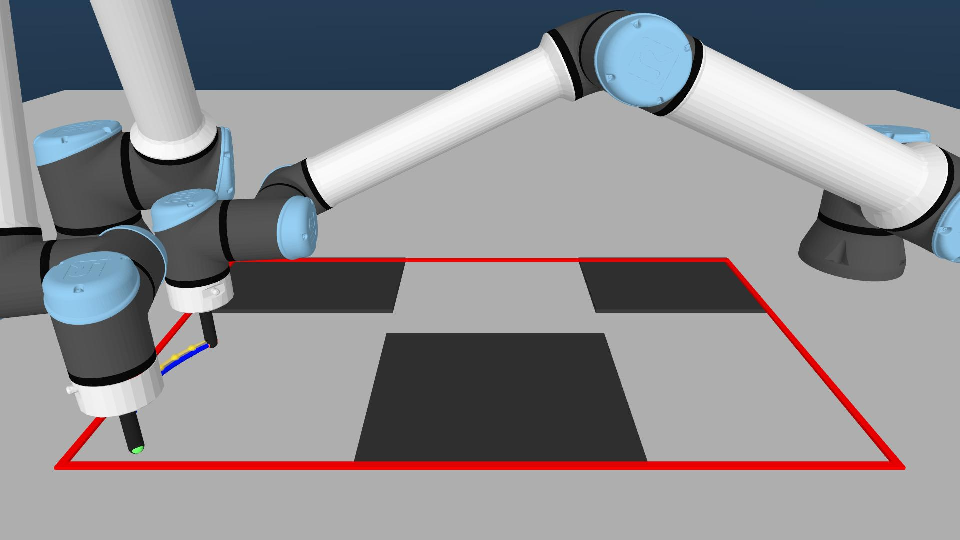
\includegraphics[width=0.21\textwidth]{figures/mujoco/scenario_05/end.pdf} \\ \hline
        \textbf{7} &
        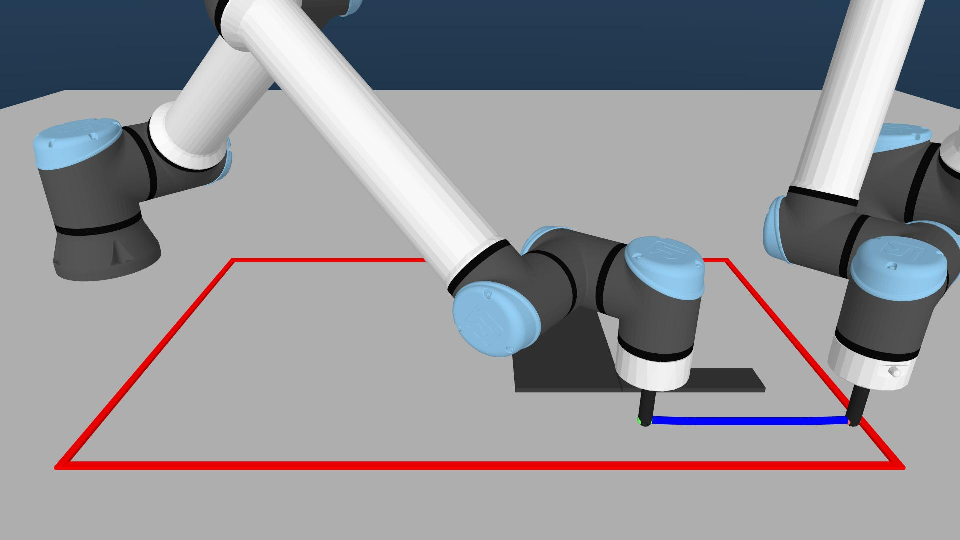
\includegraphics[width=0.21\textwidth]{figures/mujoco/scenario_07/start.pdf} &
        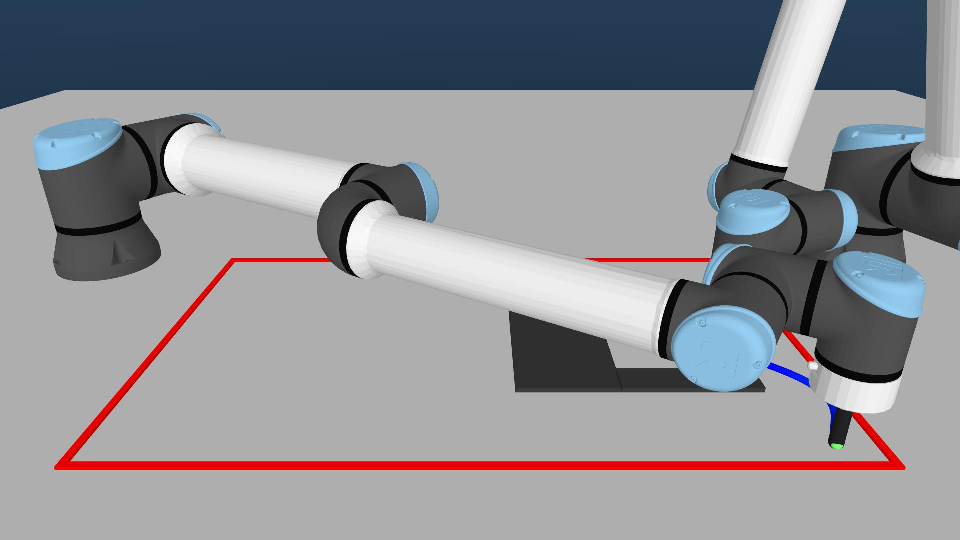
\includegraphics[width=0.21\textwidth]{figures/mujoco/scenario_07/33pct.pdf} &
        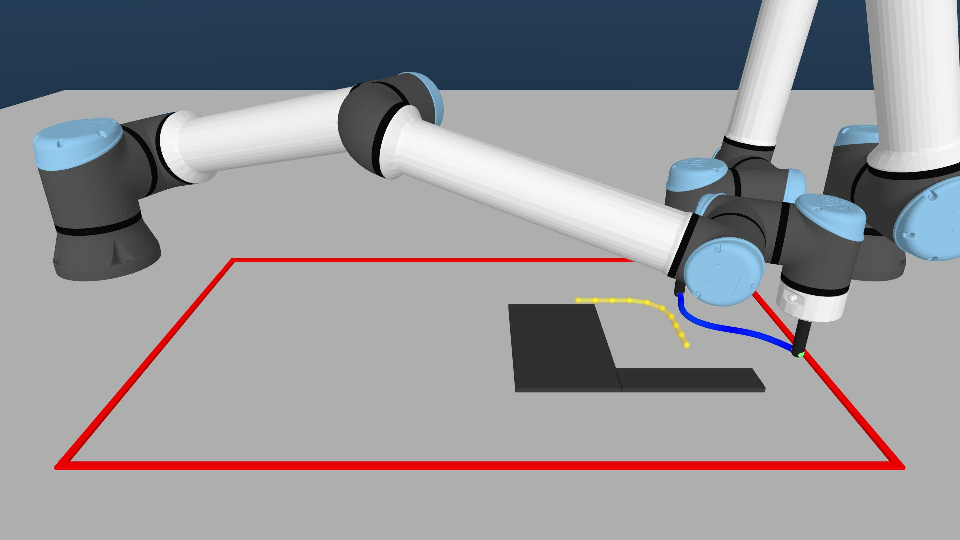
\includegraphics[width=0.21\textwidth]{figures/mujoco/scenario_07/67pct.pdf} &
        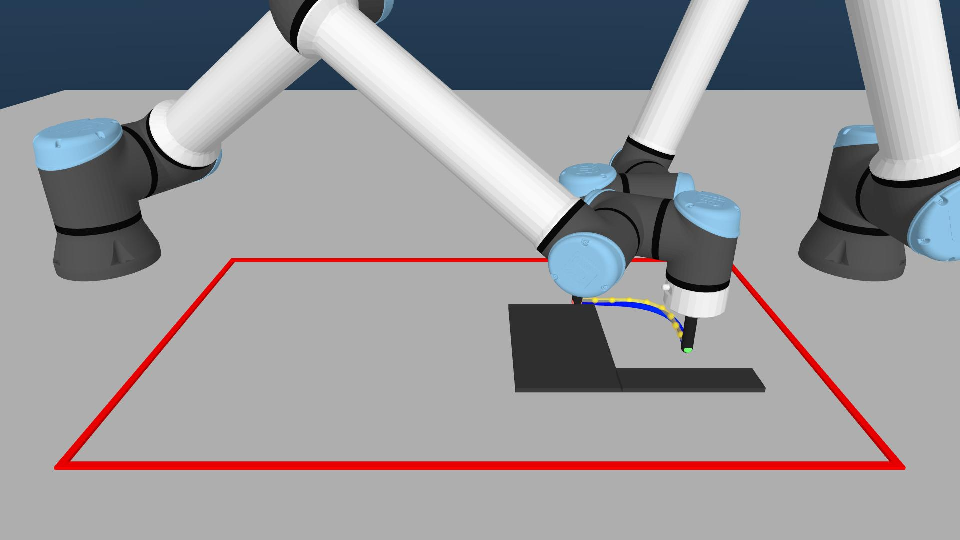
\includegraphics[width=0.21\textwidth]{figures/mujoco/scenario_07/end.pdf} \\ \hline
        \textbf{9} &
        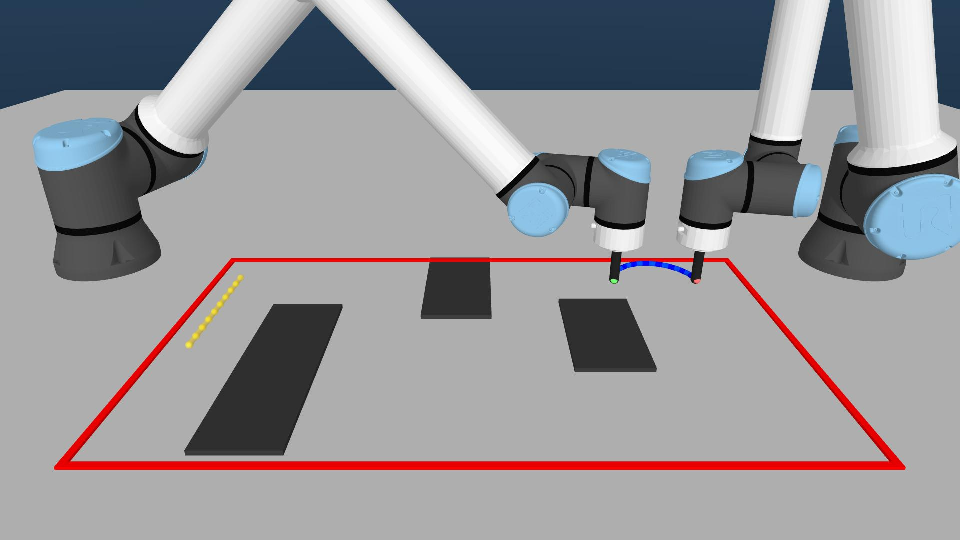
\includegraphics[width=0.21\textwidth]{figures/mujoco/scenario_09/start.pdf} &
        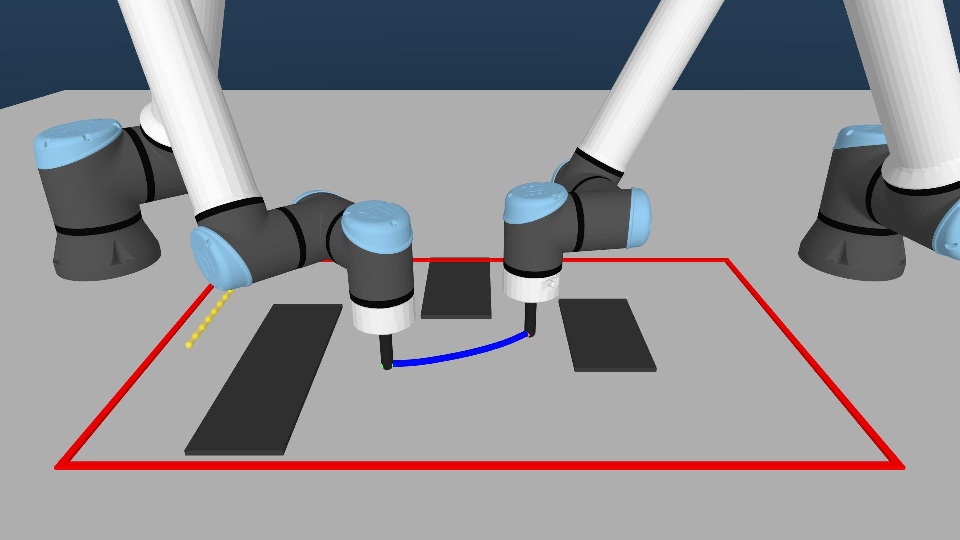
\includegraphics[width=0.21\textwidth]{figures/mujoco/scenario_09/33pct.pdf} &
        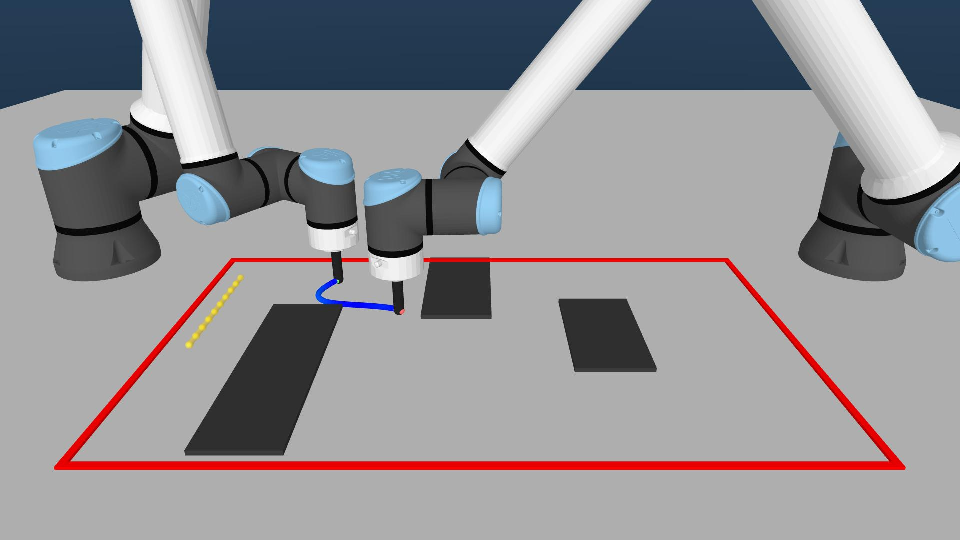
\includegraphics[width=0.21\textwidth]{figures/mujoco/scenario_09/67pct.pdf} &
        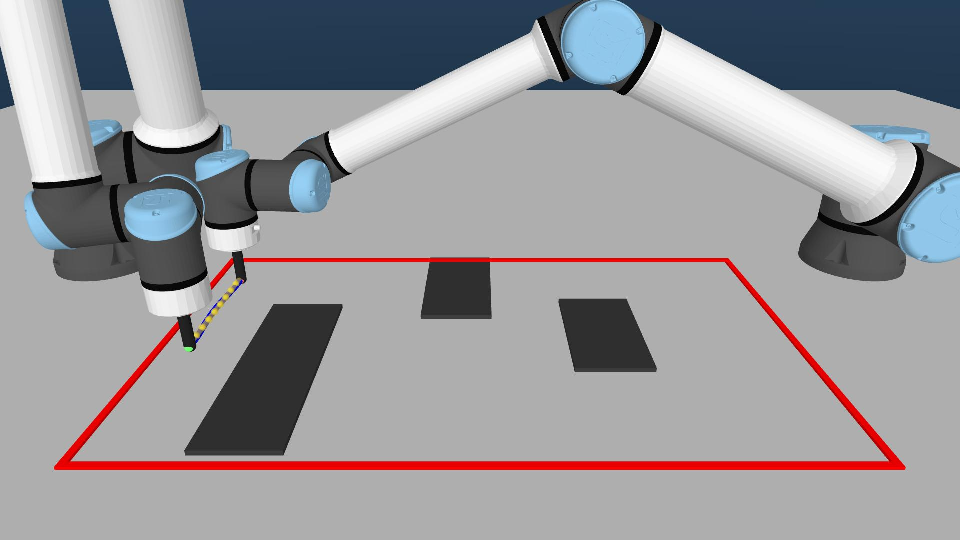
\includegraphics[width=0.21\textwidth]{figures/mujoco/scenario_09/end.pdf} \\ \hline
        \textbf{10} &
        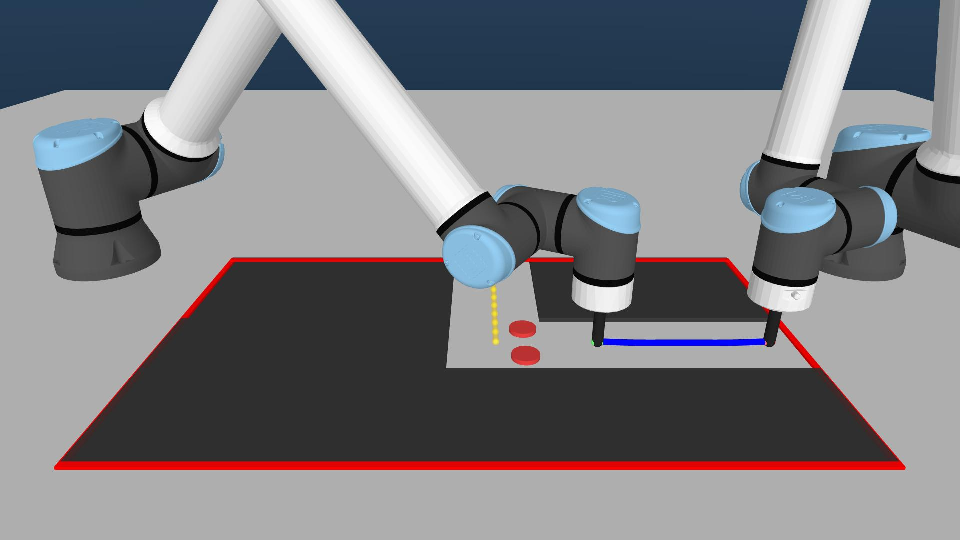
\includegraphics[width=0.21\textwidth]{figures/mujoco/scenario_10/start.pdf} &
        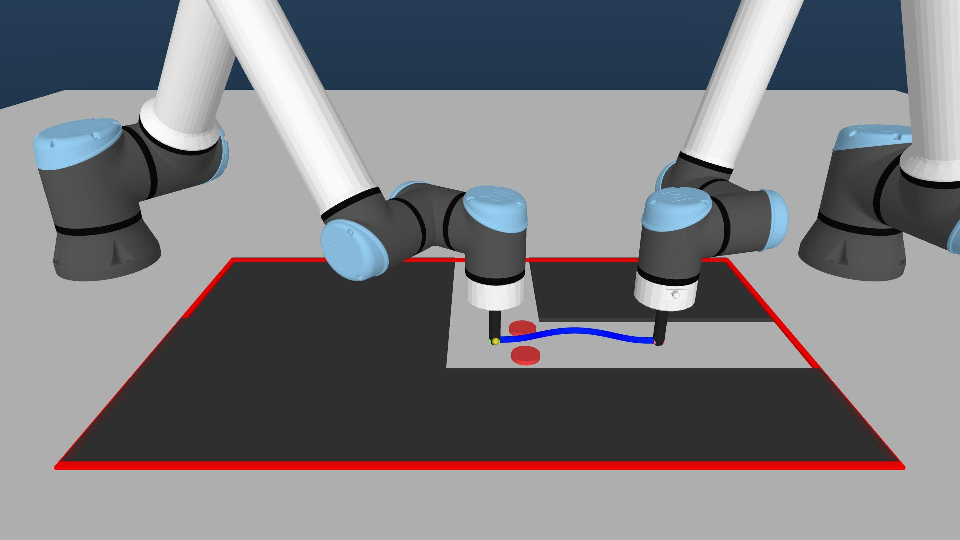
\includegraphics[width=0.21\textwidth]{figures/mujoco/scenario_10/33pct.pdf} &
        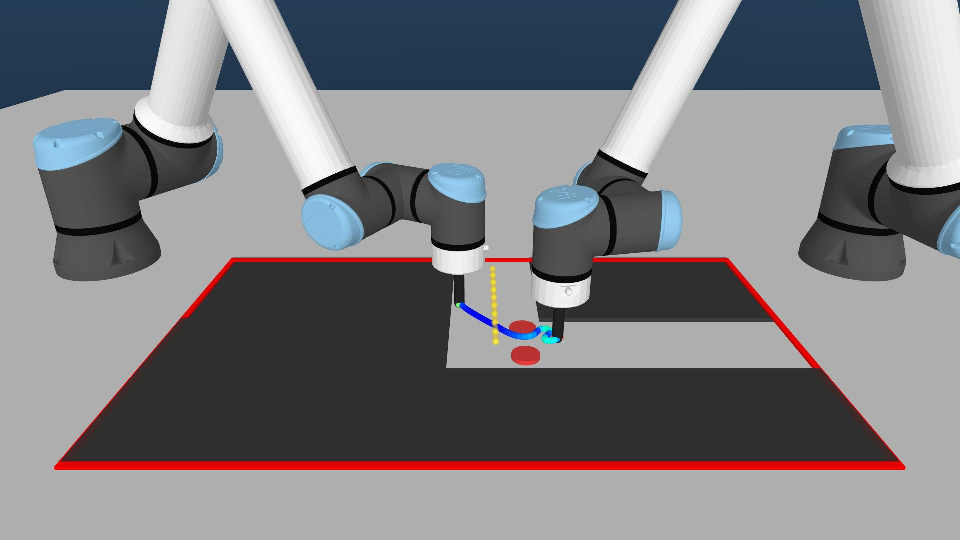
\includegraphics[width=0.21\textwidth]{figures/mujoco/scenario_10/67pct.pdf} &
        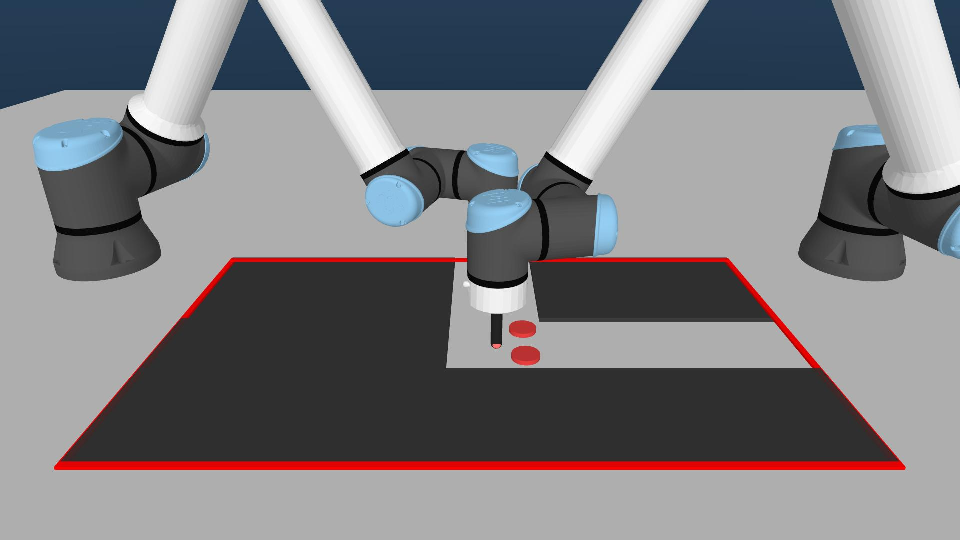
\includegraphics[width=0.21\textwidth]{figures/mujoco/scenario_10/end.pdf} \\ \hline
    \end{tabular}
    \caption{Execution snapshots for the validation scenarios. Each row shows the simulated cable manipulation at the start, two intermediate, and the end configurations.}
    \label{fig:robot_sc}
\end{figure*}

The simulated executions produce final \(\mathrm{RMSE}\) configuration errors between 1.60~mm and 4.66~mm.
For the considered cable length $L=0.27$~m, this corresponds to approximately 0.59--1.73\% of the cable length.
The maximum point-wise error ranges from 2.31~mm to 7.81~mm, or approximately 0.86--2.89\% of the cable length.
These values indicate that the executed cable shape remains close to the planned goal in the tested quasi-static replay conditions.

The error values also reflect the geometry of the tasks.
\textbf{Scenario~4} has the lowest \(\mathrm{RMSE}\), 1.60~mm, which is consistent with a smoother deformation and relatively simple endpoint motion.
\textbf{Scenarios~7} and~\textbf{9} have higher \(\mathrm{RMSE}\), 4.66~mm and 4.58~mm, respectively.
These cases require stronger deformation and larger cumulative endpoint motion, so small effects from cable elasticity, contact response, and numerical settling have a larger influence on the final configuration. Figure~\ref{fig:robot_sc} shows representative executions at the start, two intermediate stages, and the final state. The manipulation-validation records are available at \url{https://github.com/KaramAlmaghout/gcr}.



\section{Discussion}
\label{sec:discussion}

The results show that the proposed GCR planner can generate feasible routing
paths for a cable-like deformable linear object in two-dimensional cluttered
environments. The main contribution of the method is that it plans in the space
of complete cable configurations rather than only in the space of endpoint
positions. This allows the planner to reason about the shape of the whole cable,
including local segment deformation, bending, static collision avoidance, and
transition feasibility between consecutive configurations.

A central aspect of the formulation is that every accepted edge, and not only
every vertex, is validated: because each neighboring pair of configurations is
checked as a local deformation through the swept-envelope condition, the
resulting path is more suitable for execution than a sequence of independently
valid cable shapes.

The ordered edge-feasibility condition additionally guarantees that the endpoint correspondence used by the planner is preserved in the final path. This matters for dual-arm manipulation, where each cable endpoint is assigned to a specific end-effector and swapping the correspondence would change the executed motion.

The combination of APF-biased sampling and bidirectional tree search provides a
practical balance between exploration and guidance. The APF component improves
the quality of sampled configurations by moving them toward the opposite tree
and away from obstacle regions. At the same time, the planner does not rely on
APF descent alone; the bidirectional tree structure preserves global exploration
and allows the search to recover from local geometric restrictions.

The projected elastic relaxation step contributes to the mechanical plausibility
of the generated configurations. It corrects APF-biased samples by preserving
local segment structure and discrete curvature while keeping the candidate close
to the sampled direction. This relaxation is not intended to replace a full
physical cable simulator. Instead, it provides a computationally efficient
correction step that makes sampled configurations more consistent with the
discrete cable model before they are validated and inserted into the tree.

In the benchmark, more constrained scenarios required more iterations and longer planning time, which is expected because narrow passages and obstacle-dense regions reduce the number of admissible local transitions. Shortcut refinement also reduces unnecessary manipulation effort: redundant intermediate configurations are removed only when the direct transition remains feasible, and the deformation cost penalizes abrupt changes in segment vectors and discrete curvature. The final path therefore avoids unnecessary cable reshaping and provides a short sequence of deformation-feasible manipulation steps.

In the manipulation validation, the simulated robots followed the endpoint references and reproduced the planned target cable shapes with final errors below 5~mm RMSE, indicating that the planned sequences are executable by endpoint tracking alone under quasi-static conditions.

The present formulation defines a focused scope for the first implementation of
GCR and also indicates several directions for further development. In this work,
the planner is evaluated for two-dimensional planar routing with known static
obstacles. This setting is relevant to quasi-planar manipulation tasks, but
future extensions should consider three-dimensional cable routing, out-of-plane
motion, torsion, and contact interactions. The current cable model is
geometric and quasi-static: segment and curvature regularization are used to
preserve locally plausible shapes, while forces, stress limits, frictional
contacts, and dynamic effects are not explicitly simulated during planning.
Incorporating such physical quantities would make the method applicable to a
wider range of deformable-object manipulation tasks.

The swept-envelope test used in GCR provides an efficient geometric criterion
for rejecting unsafe local transitions. Since it approximates the occupied
region during a deformation, future work should study more accurate transition
models, especially when the real cable motion differs from the assumed
interpolation. The validation presented in this paper is limited to a finite set
of planar benchmark scenarios and a simulation-based dual-arm setup. These
experiments demonstrate the feasibility of the proposed planning pipeline within
the tested conditions, while further evaluation is needed across more diverse
obstacle layouts, cable stiffness values, robot platforms, and real experimental
setups.

The proposed planner is most directly applicable to tasks where a flexible
linear object must be routed through a cluttered but mainly planar workspace.
Examples include robotic cable routing in electrical cabinet assembly, wire
harness installation, routing of flexible tubes or hoses in manufacturing, and
planning intermediate shapes for dual-arm manipulation of ropes, wires, or
similar objects. In such applications, GCR can serve as a supervisory planner
that produces a sequence of feasible cable configurations, while a lower-level
controller tracks the corresponding endpoint motions and compensates for
execution errors.

\section{Conclusion}
\label{sec:conclusion}

This paper presented GCR, a global planner for routing cable-like deformable
linear objects in two-dimensional cluttered environments. The method represents
the cable as an ordered polygonal chain and searches directly in the corresponding
configuration space. This allows the planner to evaluate not only the feasibility
of individual cable shapes, but also the feasibility of local deformations between
consecutive configurations.

The proposed planning pipeline combines bidirectional tree search, APF-guided
configuration sampling, projected elastic relaxation, ordered transition
validation, and shortcut refinement. The benchmark results showed that the
planner generated feasible paths in the tested planar scenarios, while the
refinement stage reduced redundant intermediate configurations and avoided
unnecessary deformation. The simulation-based manipulation validation further indicated that the resulting paths can be converted into endpoint references that reproduce the target cable shapes with small final errors under the tested conditions.

Future work will focus on extending the formulation to three-dimensional
environments, incorporating richer physical models of cable deformation and
contact, and evaluating the planner on real robotic systems.





\bibliographystyle{apalike}
\bibliography{ref}

\end{document}
